\documentclass[a4paper, 11pt, openright]{report}
\RequirePackage[utf8]{inputenc} % input unicode
\RequirePackage[english]{babel}
\usepackage{amsthm}
\usepackage{amsmath}
\usepackage{amssymb}
\usepackage{amscd}
\usepackage{array}
%\usepackage{multicol}
\usepackage{bm}
\usepackage{bbm}
\usepackage{mathrsfs}
\usepackage{standalone}
\usepackage{cancel}
\usepackage{array}
\usepackage{enumitem}
\usepackage[toc]{appendix}
\usepackage{hyperref}
\hypersetup{
    colorlinks=true, 
    linktoc=all,    
    linkcolor=black}
\usepackage{minted}
\usepackage{subfig}
\usepackage{mathtools} %necessario per \mathclap
\usepackage[rgb,hyperref,dvipsnames]{xcolor} % necessario per \definecolor
\usepackage[most]{tcolorbox} % fa qualcosa che ammetto non ricordo, però previene problemi di compatibilità con xcolor
\usepackage[framemethod=default]{mdframed}
\usepackage{tikz-cd}
\usepackage{tikz}
\usepackage[scr=rsfs]{mathalpha}
\usepackage[final]{pdfpages}
\usepackage{pgfplots,pgfplotstable}%per disegni
\usepgfplotslibrary{fillbetween}
\pgfplotsset{compat=1.16}
\usepackage{float}%per posizionamento disegni
\usetikzlibrary{shapes,patterns,arrows,positioning,calc,arrows.meta, bending, graphs, shadings,quotes,intersections,decorations}
\newcommand{\indep}{\perp \!\!\! \perp}
\newcommand{\prob}{\mathbb{P}}
\newcommand{\ev}[1]{\mathbb{E}\left[{#1}\right]}
\newcommand{\Z}{\mathbb{Z}}
\newcommand{\R}{\mathbb{R}}
\newcommand{\N}{\mathbb{N}}
\renewcommand{\CancelColor}{\color{red}}
\definecolor{Th}{rgb}{0.8, 0.33, 0.5}
\newmdenv[skipabove=7pt,
skipbelow=7pt,
rightline=false,
leftline=true,
topline=false,
bottomline=false,
backgroundcolor=Th!10,
linecolor=Th,
innerleftmargin=5pt,
innerrightmargin=5pt,
innertopmargin=0pt,
innerbottommargin=5pt,
leftmargin=0cm,
rightmargin=0cm,
linewidth=1pt]{ThBox}
\newtheorem{Th}{Theorem}
\newtheorem{Cor}{Corollary}
\newtheorem{Lemma}{Lemma}
\newtheorem*{Note}{Note}
\definecolor{Prop}{rgb}{0.3, 0.8, 0.5}
\newmdenv[skipabove=7pt,
skipbelow=7pt,
rightline=false,
leftline=true,
topline=false,
bottomline=false,
backgroundcolor=Prop!10,
linecolor=Prop,
innerleftmargin=5pt,
innerrightmargin=5pt,
innertopmargin=0pt,
innerbottommargin=5pt,
leftmargin=0cm,
rightmargin=0cm,
linewidth=1pt]{PropBox}
\newtheorem*{Prop}{Property}
\newtheorem*{remark}{Remark}
\newtheorem*{recall}{Recall}
\newtheorem{Proposition}{Proposition}
\definecolor{Def}{rgb}{0.3, 0.5, 0.5} 
\newmdenv[skipabove=7pt,
skipbelow=7pt,
rightline=false,
leftline=true,
topline=false,
bottomline=false,
backgroundcolor=Def!10,
linecolor=Def,
innerleftmargin=5pt,
innerrightmargin=5pt,
innertopmargin=0pt,
innerbottommargin=5pt,
leftmargin=0cm,
rightmargin=0cm,
linewidth=1pt]{DefBox}
\newtheorem{Def}{Definition}
\definecolor{Proof}{rgb}{0.5, 0.3, 0.5}
\newmdenv[skipabove=7pt,
skipbelow=7pt,
rightline=false,
leftline=true,
topline=false,
bottomline=false,
backgroundcolor=Proof!10,
linecolor=Proof,
innerleftmargin=5pt,
innerrightmargin=5pt,
innertopmargin=5pt,
innerbottommargin=5pt,
leftmargin=0cm,
rightmargin=0cm,
linewidth=1pt]{ProofBox}
\newtheorem*{Proof}{Proof}
\renewcommand{\thefootnote}{\arabic{footnote}}
%\newtheorem*{Impor}{Concetto}
\newmdenv[skipabove=7pt,
skipbelow=7pt,
rightline=false,
leftline=true,
topline=false,
bottomline=false,
backgroundcolor=orange!10,
linecolor=orange,
innerleftmargin=5pt,
innerrightmargin=5pt,
innertopmargin=0pt,
innerbottommargin=5pt,
leftmargin=0cm,
rightmargin=0cm,
linewidth=1pt]{AlgoBox}
\newtheorem{algo}{Algorithm}
\newenvironment{algorithm}[1][]{

   \begin{AlgoBox}%                  
      \ifstrempty{#1}{%                         
         \begin{algo}%                     
      }{%                                       
         \begin{algo}[#1]%                 
      }%
}{%
      \end{algo}%                          
   \end{AlgoBox}%
}
\newcommand{\dif}{\mathop{}\!\mathrm{d}}
\newcommand{\ra}{\rightarrow}
\newcommand{\iy}{\infty}
\newcommand{\mE}{\mathbb{E}}
\newcommand{\mP}{\mathbb{P}}
\newcommand{\mB}{\mathcal{B}(\mathbb{R})}
\newcommand{\mL}{\mathbb{L}}
\newcommand{\mLL}{\mathbb{L}^2(0,T)}
\newcommand{\mR}{\mathbb{R}}
\newcommand{\mC}{\mathcal{C}}
\newcommand{\mRd}{\mathbb{R}^d}
\newcommand{\mN}{\mathbb{N}}
%\newcommand{\m1}{\mathbf{1}}
\newcommand{\mF}{\mathcal{F}}
\newcommand{\mM}{\mathcal{M}}
\newcommand{\mW}{\mathcal{W}}
\newcommand{\mV}{\mathcal{V}}
\newcommand{\mA}{\mathcal{A}}
\newcommand{\mez}{\frac{1}{2}}
\newcommand{\intT}{\int_{0}^{T}}
\newcommand{\ninf}{n \ra \iy}
\newcommand{\nN}{n \in \mathbb{N}}
\newcommand{\mmN}{\mathcal{N}}
\newcommand{\BM}{(B_t)_{t\geq 0}}
\newcommand{\PX}{(X_t)_{t\geq 0}}
\newcommand{\var}{\text{Var}}
\newcommand{\cov}{\text{Cov}}
\newcommand{\BMF}{\left((B_t)_{t\geq 0},\mathcal{F}_t \right)}
\newcommand{\mFt}{\mathcal{F}_t}

\usepackage{geometry}
\geometry{a4paper, top=2.5cm, bottom=2cm, left=2cm, right=2cm} % heightrounded, bindingoffset=5mm}
\title{Partial and Stochstic Differential Equations}
\author{il Priorato di Sion illuminati da lui}
\begin{document}
	\maketitle
	\newpage
	\tableofcontents
    \newpage

    \section*{Introduction for the reader}
    The course is divided into two parts:
    \begin{itemize}
        \item SDEs: 3 CFU with professor B.Toaldo
        \item PDEs: 3 CFU with professor M.Badiale
    \end{itemize}
    These notes will follow the lectures given by the professors cited above and the notes of Professor Toaldo. We will also refer to the textbook "Brownian Motion", R.Schilling.\\
    \chapter{Construction of the Brownian Motion [Professor Toaldo]}
\section{Lecture 1}
\subsection{Overview}
We are going to deepen the analysis part of this topic with Professor Badiale. \\
Now, imagine we want to describe a random phenomenon, so we deal with a random process:
\begin{equation*}
    \begin{split}
        &(X_t)_{t \geq 0} =: X\\
        &t \mapsto X_t (\omega) \quad \text{map from index set to state space}
    \end{split}
\end{equation*}
Now, the variation is 
\begin{equation*}
    dX_t = X_{t+dt} - X_t 
\end{equation*}
Notice that we are talking heuristically, not rigorously. \\
Now, let us assume that the variation is proportional to the time variation through a constant depending on the current position $c(X_t)$. What we obtain is a differential equation, together with the initial condition:
\begin{equation*}
    \begin{split}
        & d X_t= c(X_t) dt  \\
        & X_0=x
    \end{split}
\end{equation*}
The thing is that this equation is not random, since it is deterministic once we know $dt$ and the constant. We can therefore add a noise $(Y_t)$, thus obtaining a random differential equation:
\begin{equation}
\label{eq 1}
    dX_t = c(X_t) dt + \sigma Y_t
\end{equation}
The noise can be seen as 
\begin{equation*}
    Y_t \approx \sum_{k=1}^n \frac{Z_k}{n}
\end{equation*}
Letting $n$ go to infinity, by the central limit theorem, the noise is distributed as a Gaussian random variable:
\begin{equation*}
    Y_t \stackrel{CLT}{\approx} \mathcal{N}(0,dt)
\end{equation*}
The main idea is that we are summing up a countable number of elements which constitute a very small noise, scantly affecting the entire process. Nevertheless, their entirety in sum affects the process, representing the main noise. \\     
We may want to make the noise independent of $t$ yet dependent on the time lag $dt$. 

%the variance has a precise meaning,  so we set it like above.

So now, remember that the increments of the Brownian Motion are normally distributed:
\begin{equation*}
    B_{t+dt}-B_t \sim \mathcal{N}(0,dt)
\end{equation*}
With this in mind, we can rewrite \eqref{eq 1} as 
\begin{equation*}
    dX_t = \underbrace{c(X_t) dt}_{\text{deterministic}}  + \underbrace{\sigma(X_t) dB_t}_{\text{random}}
\end{equation*}
where we are also considering $\sigma$ not constant anymore, but instead depending on the current position $X_t$.\\
Now we have an heuristic point of view of the course but mathematically we still need to define some elements to have an idea of what we are talking about. 
\begin{equation}
\label{def eq}
    dX_t = c(X_t) dt + \sigma(X_t) dB_t
\end{equation}
An additional aim is to make $c(X_t)$ and $\sigma(X_t)$ dependent on time too, namely $c_t(X_t)$ and $\sigma_t(X_t)$. \\
We try to interpret \eqref{def eq} as a classical differential equation by taking derivatives:
\begin{equation*}
    \frac{d}{dt} X_t = c(X_t) + \sigma(X_t) \frac{d}{dt}B_t
\end{equation*}
The problem is that we know that "The Brownian motion is nowhere differentiable" so this interpretation is not good mathematically. \\
Then we try with the integral form:
\begin{equation*}
    X_t- X_0 = \int_0^t c(X_t) ds + \underbrace{\int_0^t \sigma(X_t) dB_s}_{\text{Itô integral}}
\end{equation*}
which is more promising since the BM is continuous and it is reasonable to think that we can integrate it. \\
The main point here is that the Riemann integral is not sufficient, since it does not work for all $\sigma$. If we want to extend the possible choice of $\sigma$ we need another construction for the integral and this leads to the theory of \textbf{Itô integration}. We recall the notion of \textbf{Riemann-Stieltjes integral}, which basically replaces the increments $\Delta s_i$ of the Riemann integral with the ones relative to a function $g$:
\begin{equation*}
    \int_0^t f_s dg_s := \lim_{n \to \infty} \sum_{i=1}^n f(\xi_i) \Delta g(s_i)
\end{equation*}
The problem is that when $g$ is a stochastic process, the integral could not converge. That's why we need a very regular process and a new definition of integral to deal with Brownian Motion. \\
So to sum up we need 
\begin{itemize}
    \item Notion of solution
    \item Existence and Uniqueness of it
\end{itemize}
To better clarify the role of the factors $c(X_t)$ and $\sigma(X_t)$, we make use of parabolic partial differential equations, of which an example is hereby reported:
\begin{equation}
\label{equation_L}
    \frac{\partial}{\partial t} q(x,t)= L q(x,t) \hspace{0.5 cm} q(x,0)=u(x)
\end{equation}
with $x \in \mR$, where $L$ is an operator given by 
\begin{equation*}
    L= a(x)\frac{\partial}{\partial x}  + b(x) \frac{\partial^2}{\partial x^2}
\end{equation*}
In the general case, $L$ could be added some other factors (like integrals).\\
A particular case is the heat equation in which analytical methods work perfectly
\begin{equation*}
    \frac{\partial}{\partial t} q(x,t)= \frac{\partial^2}{\partial x^2} q(x,t) 
\end{equation*}
In particular, the result is given by 
\begin{equation*}
    q(x,t) = \mathbb{E}^x[u(X_t)]
\end{equation*}
from which we get 
\begin{equation*}
    dX_t=b(X_t) dt + \sigma(X_t)dB_t
\end{equation*}
$b(X_t)$ corresponds to $a(x)$, while $\sigma(X_t)$ is relative to $b(x)$. \\
So, using probability we can approach partial differential equations and get methods to solve them. \\
Now, for difficult PDE's neither analytical nor numerical methods help to solve it. For example, the following provides an approximation converging to the solution of \eqref{equation_L}
\begin{equation*}
    q(x,t) \approx \frac{1}{N} \sum_{k = 1}^N u(X_t^k)
\end{equation*}
This is the scenario for Monte Carlo method, through which we can approximate it. \\
Recalling the equation we determined above, 
\begin{equation*}
    dX_t = b(X_t) dt + \sigma(X_t)dB_t
\end{equation*}
since the randomness comes from $\sigma(X_t)dB_t$, we need to know whether the Brownian Motion exists or not. This will be the goal of this chapter, but first let us recall some definitions and notions. 
\vspace{2 cm}
\section*{Revision}
\begin{DefBox}
    \begin{Def}
    $(E, \mathcal{E})$ and $(F, \mathcal{F})$ two measurable spaces, then 
    \begin{equation*}
        \begin{split}
        E \times F = \{(x,y): x \in E, y \in F\}\\
        A \subset E, B \subset F \quad A \times B = \{(x,y): x \in A, y \in B\}   \\    
        \mathcal{E}\otimes  \mathcal{F} = \sigma(\text{measurable rectangles})\\
        A \in \mathcal{E}, B\in \mathcal{F} \quad A\times B  \quad \text{ measurable rectangle}
        \end{split}     
    \end{equation*}
\end{Def}
\end{DefBox}
This isn't enough for stochastic processes since we need an infinite version:
\begin{DefBox}
    \begin{Def}
    $T$ arbitrary set ( $T=[0, \infty)$ ). For each $t \in T$, consider $(E_t, \mathcal{E}_t)$ a measurable space, $x_t \in E_t$ for each $t\in T$, $x:=(x_t)_{t \in T}$ is a function on $T$. \\
    $T \owns t \mapsto x_t \in E_t$ (where usually $E_t \equiv E \quad \forall t \in T$ for stochastic processes).\\
    $F:=\{\text{set of all such functions  } x = (x_t)\}$ is the \textbf{product space}.
\end{Def}
\end{DefBox}

\begin{DefBox}
    \begin{Def}
    A measurable rectangle in $F$ is a subset of $F$
    \begin{equation*}
        \bigtimes_{t \in T} A_t =\{x \in F: x_t\in A_t \quad \forall t \in T\}
    \end{equation*}
    where $A_t$ differs from $E$ ($E_t$) only for a finite number of $t \in T$.
\end{Def}
\end{DefBox}
Then a rectangle is measurable if $A_t \in \mathcal{E}_t$ for every $t \in T$, and the product sigma algebra is the one generated by all measurable rectangles:
\begin{equation*}
    \otimes_{t \in T} \mathcal{E}_t =\sigma \{\text{measurable rectangles}\}
\end{equation*}
\paragraph{Example} \begin{equation*}
    \begin{split}
        &E=\mR \hspace{1 cm} T=[0,\infty)\\
        &(\mR^{[0, \infty)}, \mathcal{B}^{[0, \infty)})
    \end{split}
\end{equation*}
The Borel-sigma algebra is countably measurable since it is generated by countably many measurable rectangles. It is a countable union of functions with \emph{finite} fixed positions. 
\begin{PropBox}
    \begin{Proposition}
    Let $(\Omega, \mathcal{A})$ be a measurable space and let $(F,\mathcal{F}) = \bigtimes _{t \in T} (E_t, \mathcal{E}_t)$. For each $t\in T$ let $f_t: \Omega \to E_t$. For each $\omega \in \Omega$ define $f(\omega)$ to be the point $(f_t(\omega))_{t \in T}$ in F. \\
    Then $f: \Omega \to F$ is $\mathcal{A}$-measurable (on $(A, \mathcal{F})$) $\iff$ $f_t$ is $\mathcal{A}$-measurable for every $t \in T$ (on $(A, \mathcal{E}_t)$).
\end{Proposition}
\end{PropBox}
Hence, we can characterize the measurability of a function on the product space based on the measurability of its components on a single set $E_t$ for every $t \in T$. 
\subsection{Brownian Motion}
Let $(\Omega, \mathcal{A}, \mathbb{P})$ be a probability space. 
\begin{DefBox}
    \begin{Def}
    A $d$-dimensional stochastic process $(B_t)_{t \geq 0} = : B$ on $(\Omega, \mathcal{A}, \mathbb{P})$ is a Brownian Motion if:
    \begin{itemize}
        \item $B_0 = 0$ almost surely 
        \item independent increments: $B_{t_i} - B_{t_{i-1}} \coprod$ for $i = 1, \ldots, n \quad n \in \mathbb{N}, t_0 < \ldots < t_n$
        \item stationary increments: $0 \leq s \leq t: B_t - B_s \sim B_{t-s}$
        \item Gaussian increments: $B_t - B_s \sim \mathcal{N}(0, (t-s) \mathbbm{1})$
        \item the trajectories $t \mapsto B_t(\omega)$ are continuous $\forall \omega \in \Omega$. 
    \end{itemize}
\end{Def}
\end{DefBox}
We will see that the course is greatly centered around the probability space $(C_0, \mathcal{B}_{C_0}, \mathbb{P})$ called Wiener space, where $C_0$ is the set of continuous functions, $\mathcal{B}_{C_0}$ is the Borel sigma-algebra and $\mathbb{P}$ is the Wiener measure.

\newpage

\section{Lecture 2}
We wrote the equation \eqref{def eq} whose solution is $X_t$ and in particular we said that the term $\sigma(X_t) dB_t$ adds randomness. The problem is that we need to be sure about the existence of the Brownian Motion to write and treat such an equation. Now, we are going to construct it. \\  
Actually, to construct and prove the existence of the BM there are two approaches:
\begin{itemize}
    \item the \textbf{Lévy construction}, which only works for the Brownian Motion
    \item the \textbf{canonical construction}, which is used for many processes and consists in fixing a probability space $(C_0(I)), \ldots, \ldots)$ with $C_0(I)$ space of continuous functions, then identifying a $\sigma$-algebra and a probability measure to obtain a BM. To do so, we use $X(\omega) = \omega$ as a process.
\end{itemize}
We want to find a probability space $(\Omega, \mathcal{F}, \mP)$ and a r.v. on it satisfying the definition. The Kolmogorov Theorem allows to do it. Recall first that we are going to work with 
\begin{equation*}
    \mathbb{R}^I = \{\omega: I \to \mathbb{R}\} = \bigtimes _{t \in I} \mathbb{R}, \quad \mathcal{B}^I(\mathbb{R}) = \bigtimes_{t \in I} \quad \text{ product $\sigma$-algebra }
 \mathcal{B}(\mathbb{R})
 \end{equation*}
 considering therefore the space $(\mathbb{R}^I, \mathcal{B}^I(\mathbb{R}))$.
\begin{ThBox}
    \begin{Th}[Kolmogorov Theorem]
    For each $t_1, \dots, t_n \geq 0$ and for every $n \in \mathbb{N}, $ with $t_j \neq t_k$, $j \neq k$, let $p_{t_1, \dots, t_n}(\cdot, \dots, \cdot)$ be a probability measure on $(\mR^n, \mathcal{B}(\mR^n))$ (for fixed times $t_i$). \\
    Assume that this family satisfies the so-called consistency conditions:
    \begin{enumerate}
        \item $p_{t_1, \dots, t_n}(A_1 \times  \dots \times  A_n) = p_{t_{\sigma(1)}, \dots, t_{\sigma(n)}}(A_{\sigma(1)} \times  \dots \times  A_{\sigma(n)})$ where $\sigma:\{1, \dots, n\} \to \{1, \dots, n\} $ is a permutation of $\{1, \ldots, n\}$;
        \item $p_{t_1, \dots, t_{n-1}}(A_1\times  \dots \times  A_{n-1}) =p_{t_1, \dots, t_{n-1}, t_n}(A_1\times  \dots \times  A_{n-1}\times \mR) $
    \end{enumerate}
    Then there exists a (unique) probability measure $\mu$ on the product space $(\mR^{[0,\infty)}, \mathcal{B}^{[0,\infty)}(\mR))$ such that the canonical process $X=(X_t)_{t \geq 0}$ with $X_t(\omega)= \omega(t)$ has finite dimensional distribution 
    \begin{equation*}
        \mP(X_{t_1}\in A_1, \dots, X_{t_n} \in A_n)= p_{t_1, \dots, t_n}(A_1 \times \dots \times  A_n)
    \end{equation*}
    for any $t_1, \dots, t_n$, $n \in \mathbb{N}$.
\end{Th}
\end{ThBox}

\begin{PropBox}
    \begin{Cor}
    There exists a unique measure $\mu$ on $(\mR^I,\mathcal{B}^I(\mR) )$ such that the canonical process $X=(X_t)_{t \geq 0}$ satisfies $X_0=0$ almost surely, has  stationary and independent increments. 
\end{Cor}
\end{PropBox}
\begin{ProofBox}
\begin{proof}[Sketch of the proof]
    Let $p_{t_1, \dots, t_n}$ be Gaussian $(\underline{0}, C)$, $C_{ij}= min(t_i, t_j)$. The Gaussian distribution satisfies the consistency conditions. 
\end{proof}
\end{ProofBox}
Now, the next thing we need is the continuity of trajectories. Define
\begin{equation*}
    C_0=\{\omega \in \mathbb{R}^I \text{s.t. } \omega \text{ is continuous and } \omega(0) = 0\}
\end{equation*}
We would like to have $\mu(C_0) = 1$, but we are not sure about its validity. The problem is that the product $\sigma$-algebra is too small and the Kolmogorov theorem holds on the product $\sigma$-algebra.
\begin{PropBox}
    \begin{Lemma}
    For every $I \in \mathcal{B}^I(\mathbb{R})$ there exists on at most countable set $S \subset [0,+\infty)$ s.t. $v \in I, \omega \in \mathbb{R}^I, v|_S = \omega |_S$, then $\omega \in I$. 
\end{Lemma}
\end{PropBox}
Therefore, $C_0 \notin \mathcal{B}^{[0,+\infty)}$. So, not all the elements contain continuous functions and hence we cannot compute the probability $\mu(C_0)$. The solution to this problem is provided by the following theorem.
\begin{ThBox}
    \begin{Th}[Kolmogorov-Centsov]
    Let \((X_t)_{t \geq 0}\) be a \(d\)-dimensional process in \((\Omega, \mathcal{F}, \mathbb{P})\). If there are constants \(c > 0\), \(\alpha > 0\), and \(\beta > 0\) such that:
    \begin{equation*}
        \mathbb{E} \left( |X_t - X_s|^\alpha \right) \leq c |t - s|^{1 + \beta}, \quad \text{for all } s, t \geq 0
    \end{equation*}
then \(X_t\) has a version with exclusively only continuous trajectories.
\end{Th}
\end{ThBox}
Recall that a version of a process is a process itself $(Y_t)_{t \geq 0}$ such that 
\begin{equation*}
    \mathbb{P}(X_t = Y_t) = 1 \quad \text{ for all } t \geq 0
\end{equation*}
\begin{equation*}
    \begin{split}
        & (\mathbb{R}^{[0, +\infty)}, \mathcal{B}^{[0,+\infty)}(\mathbb{R}), \mu) \quad X \rightarrow Y \\
        & Y: \mathbb{R}^{[0,+\infty)} \hookrightarrow C_0 \\
        & (C_0, \mathcal{B}(C_0), \mathbb{P})
    \end{split}
\end{equation*}
If we put together these two results we get the continuity of trajectories! \\
Take $(\mathbb{R}^I, \mathcal{B}^I(\mathbb{R}), \mu)$ and use $Y=(Y_t)_{t \in I}$ which is the Kolmogorov-Centsov version of the canonical process on $(\mathbb{R}^I, \mathcal{B}^I(\mathbb{R}))$. Then, take $(C_0(I), \mathcal{B}(C_0(I)), P)$ where $P$ is the Wiener measure and $B = (B_t)_{t \geq 0}$ is the canonical process on $(C_0(I), \mathcal{B}(C_0(I)), P)$. 

\chapter{Properties of the Brownian Motion [Professor Toaldo]}
In this chapter we want to deepen the main known results about the oscillation of the Brownian Motion, whose trajectories are pretty irregular in time. \\
In particular, the basic notions to keep in mind are the following
\begin{itemize}
    \item $t \mapsto B_t(\omega)$ is continuous 
    \item almost surely, $t \mapsto B_t(\omega)$ has no points where it is differentiable
    \item $t \mapsto B_t(\omega)$ has no bounded variation almost surely on any finite interval $[a,b]$, that is the vertical distance run by the BM in finite time from $a$ to $b$ is always infinity
    \item almost surely, the BM has no monotone interval, that is the probability that there exists an interval such that the BM is monotone inside equals $0$. 
\end{itemize}
Consider a continuous function $f:[0,+\infty) \rightarrow \mathbb{R}$ and suppose we want to know the distance run by $f$ on $[0,t]$, that is the oscillation over this interval. The latter should be given approximately by $f(t) - f(0)$, which can be roughly approximated in turn by the sum of oscillations of $f$ over small consecutive intervals $[t_0, t_1] \ldots [t_{n-1}, t_n]$ with $0 = t_0 \leq \ldots \leq t_n = t$. 
\begin{equation*}
    |f(t_1) - f(t_0)|+|f(t_2) - f(t_1)|+ \ldots
\end{equation*}
We could try to improve the quality of the approximation by letting the amplitude of the intervals go to $0$. 
\begin{DefBox}
    \begin{Def}[strong $p$-variation]
    Let $f:[0,+\infty) \to \mathbb{R}$ be a function on $\Pi := \{0 = t_0 < t_1 < \ldots < t_n = t\}$, a partition of $[0,t]$ with mesh $|\Pi| := \max_j |t_j - t_{j-1}|$. For $p > 0$ we call 
    \begin{align*}
        S_p^\Pi(f,t) &= \sum_{t_j \in \Pi} |f(t_j) - f(t_{j-1})|^p\\
        &= \sum_{j=1}^n |f(t_j) - f(t_{j-1})|^p
    \end{align*}
    is the p-variation sum of $f$ along $\Pi$. \\
    We call $\text{VAR}_p(f,t) := \sup\{S_p^\Pi(f,t): \Pi \text{ partition of } [0,t]\}$ the strong (or total) $p$-variation.
\end{Def}
\end{DefBox}

\begin{remark}
    If $\text{VAR}_1(f,t) < \infty$, then $f$ is of bounded variation.  
\end{remark}

\begin{DefBox}
    \begin{Def}[$p$-variation]
    Let \( f \colon [0, \infty) \to \mathbb{R} \) and let \( (\Pi_n)_{n \in \mathbb{N}} \) be a sequence of partitions of \([0, t]\) with \( |\Pi_n| \to 0 \) as \( n \to \infty \). 

Then, the \(p\)-variation of \(f\) over \([0,t]\) is defined as:

\[
\text{Var}_p(f, t) := \lim_{n \to \infty} S_p^{\Pi_n}(f, t)
\]

where \( S_{\Pi_n}(f, t) \) denotes the sum associated with the partition \(\Pi_n\).
\end{Def}
\end{DefBox}
We want $f$ to be the Brownian Motion path, depending on the trajectories:
\begin{equation*}
        f_t \equiv B_t(\omega)   
\end{equation*}
This means that we should clarify in which sense the limit which defines the p-variation exists. That's, in particular, because $(\Pi_n)_{n \in \mathbb{N}}$ are typically not allowed to depend on $\omega$.       \\
The main result is the following.
\begin{ThBox}
    \begin{Th}[Quadratic variation of BM]
    Let $(B_t)_{t \geq 0}$ be a one-dimensional Brownian Motion. Let $(\Pi_n)_{n \in \mathbb{N}}$ be a sequence of partitions of $[0,t]$ s.t. $|\Pi_n| \rightarrow 0$. Then
    \begin{equation*}
        VAR_2(B,t) := L^2-\lim_{n \rightarrow +\infty} S_2^{\Pi_n}(B,t) = t
    \end{equation*}
\end{Th}
\end{ThBox}
This means that the quadratic variation of the Brownian Motion equals $t$ in the $L^2$ sense. \\
Before providing the proof of the theorem, we remark that
\begin{remark}
    The sequence $\Pi_n$ is not allowed to depend on $\omega \in \Omega$. It is indeed possible to prove that for almost every $\omega \in \Omega$ there exists a sequence of partitions $(\Pi_n(\omega))_{n \in \mathbb{N}}$ of $[0,t]$ with $|\Pi_n(\omega)|\rightarrow 0$ such that
    \begin{equation*}
        \lim_{n \rightarrow \infty} S_2^{\Pi_n(\omega)}(B(\cdot, \omega), t) = \infty \quad \text{ a.s. }
    \end{equation*}
    Moreover, this implies also that VAR$_2(B(\cdot, \omega), t) = \infty$ almost surely. 
\end{remark}
\begin{ProofBox}
    \begin{proof}
    The thesis is 
    \begin{equation*}
        \lim_{|\Pi| \rightarrow 0} \mathbb{E}|S_2^\Pi(B,t) - t|^2 = 0
    \end{equation*}
    which is the $L^2$ norm. \\
    Let a partition $\Pi = \{0 = t_0 < t_1 < \ldots < t_n = t\}$ of $[0,t]$ be fixed and notice that
    \begin{equation*}
        \mathbb{E}(S_2^\Pi(B,t)) = \sum_{j=1}^n \mathbb{E}(B{t_j} - B_{t_j-t_{j-1}})^2 = \sum_{j=1}^n(t_j-t_{j-1}) = t
    \end{equation*}
    Then, by the independence of the increments and $\sum_{j=1}^n(t_j-t_{j-1}) = t$:
    \begin{align*}
        \mathbb{E}(S_2^\Pi(B,t)-t)^2 &= \mathbb{V}ar(S_2^\Pi(B,t)) \\
        &= \sum_{j=1}^{n} \mathbb{E} [(B_{t_j} - B_{t_{j-1}})^2 - (t_j - t_{j-1})]^2 \\
        &= \sum_{j=1}^{n} \mathbb{E} [B^2_{t_j - t_{j-1}} - (t_j - t_{j-1})]^2 \quad \text{by stationarity of the increments}\\
        &= \sum_{j=1}^{n} (t_j - t_{j-1})^2 \mathbb{E} [B_1^2 - 1]^2 \quad \text{since $B_t \stackrel{\text{d}}=\sqrt{t} B_1$}\\
        &\leq c \sum_{j=1}^{n} (t_j - t_{j-1}) (t_j - t_{j-1}) \\
        & \leq c \underbrace{|\Pi| }_{\text{ bound with maximum }} \sum_{j=1}^{n} |t_j - t_{j-1}| = c |\Pi| t \rightarrow 0 \quad |\Pi| \rightarrow 0
    \end{align*}
\end{proof}
\end{ProofBox}
\section*{Some other notions}
Since the $L^2$-convergence implies the existence of an almost surely convergent subsequence, the previous result also proves that there exists a subsequence $\Pi_{n_k}$ such that $S_2^{\Pi_{n_k}}(B,t) \rightarrow t$ almost surely. 
\begin{PropBox}
    \begin{Proposition}
    \begin{equation*}
        S_2^{\Pi_n}(B,t) \xrightarrow{L^2} t
    \end{equation*}
    There exists $(\Pi_{n_k})_{k \in \mathbb{N}}$ s.t. $S_2^{\Pi_{n_k}} (B,t) \xrightarrow{ \text{ a.s. }} t$.
\end{Proposition}
\end{PropBox}
We wonder how to find such subsequence and the answer is given by the following theorem.  
\begin{ThBox}
    \begin{Th}
    Let $(\Pi_n)_{n \in \mathbb{N}}$ be a sequence of partitions of $[0,t]$ with 
        \begin{equation}
        \label{assumption}
            \sum_n |\Pi_n| < +\infty
        \end{equation}
    Then, then $S_2^{\Pi_n}(B,t) \xrightarrow{ \text{a.s.}} t, n \rightarrow \infty$.
\end{Th}
\end{ThBox}
\begin{remark}
    The assumption \ref{assumption} implies that $|\Pi_n| \rightarrow 0$ sufficiently fast.
\end{remark}
\begin{PropBox}
    \begin{Proposition}
    \begin{equation*}
        VAR_p(B,t) = +\infty \text{  a.s. } \forall t \geq 0, p \leq 2
    \end{equation*}
\end{Proposition}
\end{PropBox}
For $p=2$ it is possible to find $\Pi_n(\omega)$ s.t. $\lim_{n\rightarrow +\infty} S_2^{\Pi_n(\omega)} (B,t) = +\infty$.\\
The idea is that if we consider the distance $|b-a| > 0$ of only one trajectory we get a very bad approximation, while if instead we take all the trajectories in average we obtain a pretty good approximation in  $L^2$. 
\begin{equation*}
    \int_0^t f dg := \lim_{|\Pi| \rightarrow 0} \sum_{t_j \in \Pi} f(\xi_j)(g(t_j) - g(t_{j-1}))
\end{equation*}
with $\xi_j \in [t_{j-1}, t_j)$. If we transform it into an $L^2$ integral adding the dependence on $\omega$, then the integral now converges. This is not the true definition of Itô integral though, of which we will give an easier approach later.
\chapter{(Ir)regularity of Brownian paths [Professor Toaldo]}
\begin{DefBox}
    \begin{Def}
    A function $f:[0,+\infty) \rightarrow \mathbb{R}$ is said to be locally Holder continuous of order $\alpha \in (0,1]$ if, for every $T>0$, there is a constant $c(T)$ s.t.
    \begin{equation*}
        |f(t)-f(s)| \leq c|t-s|^\alpha \quad s,t \in [0,T]
    \end{equation*}
\end{Def}
\end{DefBox}
The function is globally Holder continuous if $c(T) = c$ does not depend on T. 
\begin{ThBox}
    \begin{Th}
    Almost all Brownian paths are nowhere locally Holder-continuous for $\alpha>\frac{1}{2}$.
\end{Th}
\end{ThBox}
\begin{ProofBox}
    \begin{proof}
    Fix $\alpha > \frac{1}{2}$. Take $I=[a,b]$. Define 
    \begin{equation*}
        \mathcal{N}_{a,b} := \{\omega \in \Omega: \exists c(\omega) \text{  s.t.  } |B(t,\omega) - B(s,\omega)| \leq c(\omega) |t-s|^\alpha \quad \forall s,t \in [a,b]\}
    \end{equation*}
    We want to prove
    \begin{equation*}
        \mathbb{P}(\cup_{a,b} \mathcal{N}_{a,b}) = 0
    \end{equation*}
    Since $a,b \in [0,+\infty)$ they can be rationals, making the union countable. Therefore, since
    \begin{equation*}
        \mathbb{P}(\cup_{a,b} \mathcal{N}_{a,b}) \leq \sum_{a,b \in \mathbb{Q}}\mathbb{P}(\mathcal{N}_{a,b})
    \end{equation*}
    we need to prove $\mathbb{P}(\mathcal{N}_{a,b})=0$. Fix $\omega \in \mathcal{N}_{a,b}$ and suppose by contradiction the function is Holder continuous of order $\alpha$. 
    \begin{align*}
        S_2^{\Pi_n}(B(\cdot,\omega), [a,b]) &= \sum_{j=1}^n (B_{t_j}(\omega) - B_{t_{j-1}}(\omega))^2\\
        &\stackrel{\omega \in \mathcal{N}_{a,b}}\leq c^2(\omega) \sum_{j=1}^n |t_j - t_{j-1}|^{2\alpha+1-1} \\
        &\leq c^2(\omega) |\Pi|^{2\alpha -1} \sum_{j=1}^n|t_j-t_{j-1}| \rightarrow 0, \quad |\Pi| \rightarrow 0 
    \end{align*}
    We recall that 
    \begin{equation*}
        \sum_{j=1}^n|t_j-t_{j-1}| = b-a
    \end{equation*}
    On the other hand, since there exists a sequence of partitions $(\Pi_n)_{n \in \mathbb{N}}$ of $[a,b]$ with 
    \begin{equation*}
        |\Pi| \rightarrow 0 \quad \text{such that} \quad S_2^{\Pi_n}(B, [a,b]) \rightarrow b-a \text{   a.s. }
    \end{equation*}
    Therefore, since it is an arbitrary partition, it follows that $\mathbb{P}(\mathcal{N}_{a,b})=0$. \\
    This leads to a contradiction and to the proof of the thesis. 
\end{proof}
\end{ProofBox}

\newpage

\section{Lecture 3}
Last time we talked about the Wiener space $(\Omega, \mathcal{A}, \mP)$, in which we considered $B_t$ a Brownian Motion. Then, we defined the p-variation of the BM.\\
Now, we are going to keep discussing about the \emph{(ir)regularity} of the BM: in particular, we concluded that if we consider just one trajectory of the BM we do not achieve regularity, while instead if we consider the entirety of them we get it together with the convergence. \\
Keep in mind the result we stated last lecture about the almost sure Holder continuity of the trajectories: the BM paths are nowhere locally Holder continuous when $\alpha > \frac{1}{2}$, which is actually valid for $\alpha = \frac{1}{2}$ too (proof too difficult).\\
Let us now state a weaker version of the Kolmogorov-Centsov theorem. 
\begin{ThBox}
    \begin{Th}
    Let $(Y_t)_{t \geq 0}$ be a random process on $\mR$ with continuous paths. Let $T>0$. If there exists finite constants $c>0$, $\beta, \gamma >0$ s.t.
    \begin{equation*}
        \mE|X_t-X_s|^\gamma \leq c|t-s|^{1+\beta} \hspace{1 cm } s, t \in [0,T]    \end{equation*}
 Then, the paths $[0,T] \owns t \mapsto X_t (\omega)$ are a.s. Holder continuous of order $\alpha \in (0, \frac{\beta}{\gamma})$ and  
 \begin{equation*}
     \mE \Big[\sup_{0 < |s-t|< 1 \ \ s,t \in [0,T]} \frac{|X_t-X_s|}{|t-s|}\Big]^\gamma< \infty \hspace{ 1 cm} \alpha \in (0, \frac{\beta}{\gamma})
 \end{equation*}
\end{Th}
\end{ThBox}
\begin{PropBox}
    \begin{Cor}
    The paths $t \mapsto B_t(\omega)$ of the BM are a.s. locally Holder continuous for $\alpha < \frac{1}{2}$
\end{Cor}
\end{PropBox}
\begin{ProofBox}
    \begin{proof}
    \begin{equation*}
    \begin{split}
    \mathbb{E}[|B_t - B_s|^n] &\stackrel{ \text{stationarity}} = \mathbb{E}[|B_{t-s}|^n] \stackrel{ \text{scaling}} = |t-s|^\frac{n}{2} \underbrace{\mathbb{E}|B_1|}_{C \text{ const.}}\\
        \mE |B_t -B_s|^\gamma &\leq c |t-s|^{1+\beta}\\
        \text{ where }\gamma= n &\hspace{0.5 cm} \beta=  \frac{n}{2}-1\\
        \alpha < \frac{\beta}{\gamma}&= \frac{1}{2}-\frac{1}{n} \hspace{1 cm}
    \end{split}      
    \end{equation*}
    and for $n$ big enough we are able to reach the desired result.
\end{proof}
\end{ProofBox}
\begin{PropBox}
    \begin{Proposition}
\label{prop 1}
    For each fixed $T > 0$, then the Brownian paths $t \mapsto B_t(\omega)$ are not differentiable at $t=T$ almost surely. 
\end{Proposition}
\end{PropBox}
The strongest version of this concept that we can achieve is the following 
\begin{PropBox}
    \begin{Proposition}
\label{prop 2}
    The sample paths $t \mapsto B_t(\omega)$ are almost surely nowhere differentiable. 
\end{Proposition}
\end{PropBox}
The proof of \eqref{prop 1} comes from Stochastic Processes course, while the one of \eqref{prop 2} is in Toaldo's notes. \footnote{page $60$-$61$ file notes from last year}

A graphic representation is provided in Figure \ref{fig_1}. 

\begin{figure}
    \begin{center}
    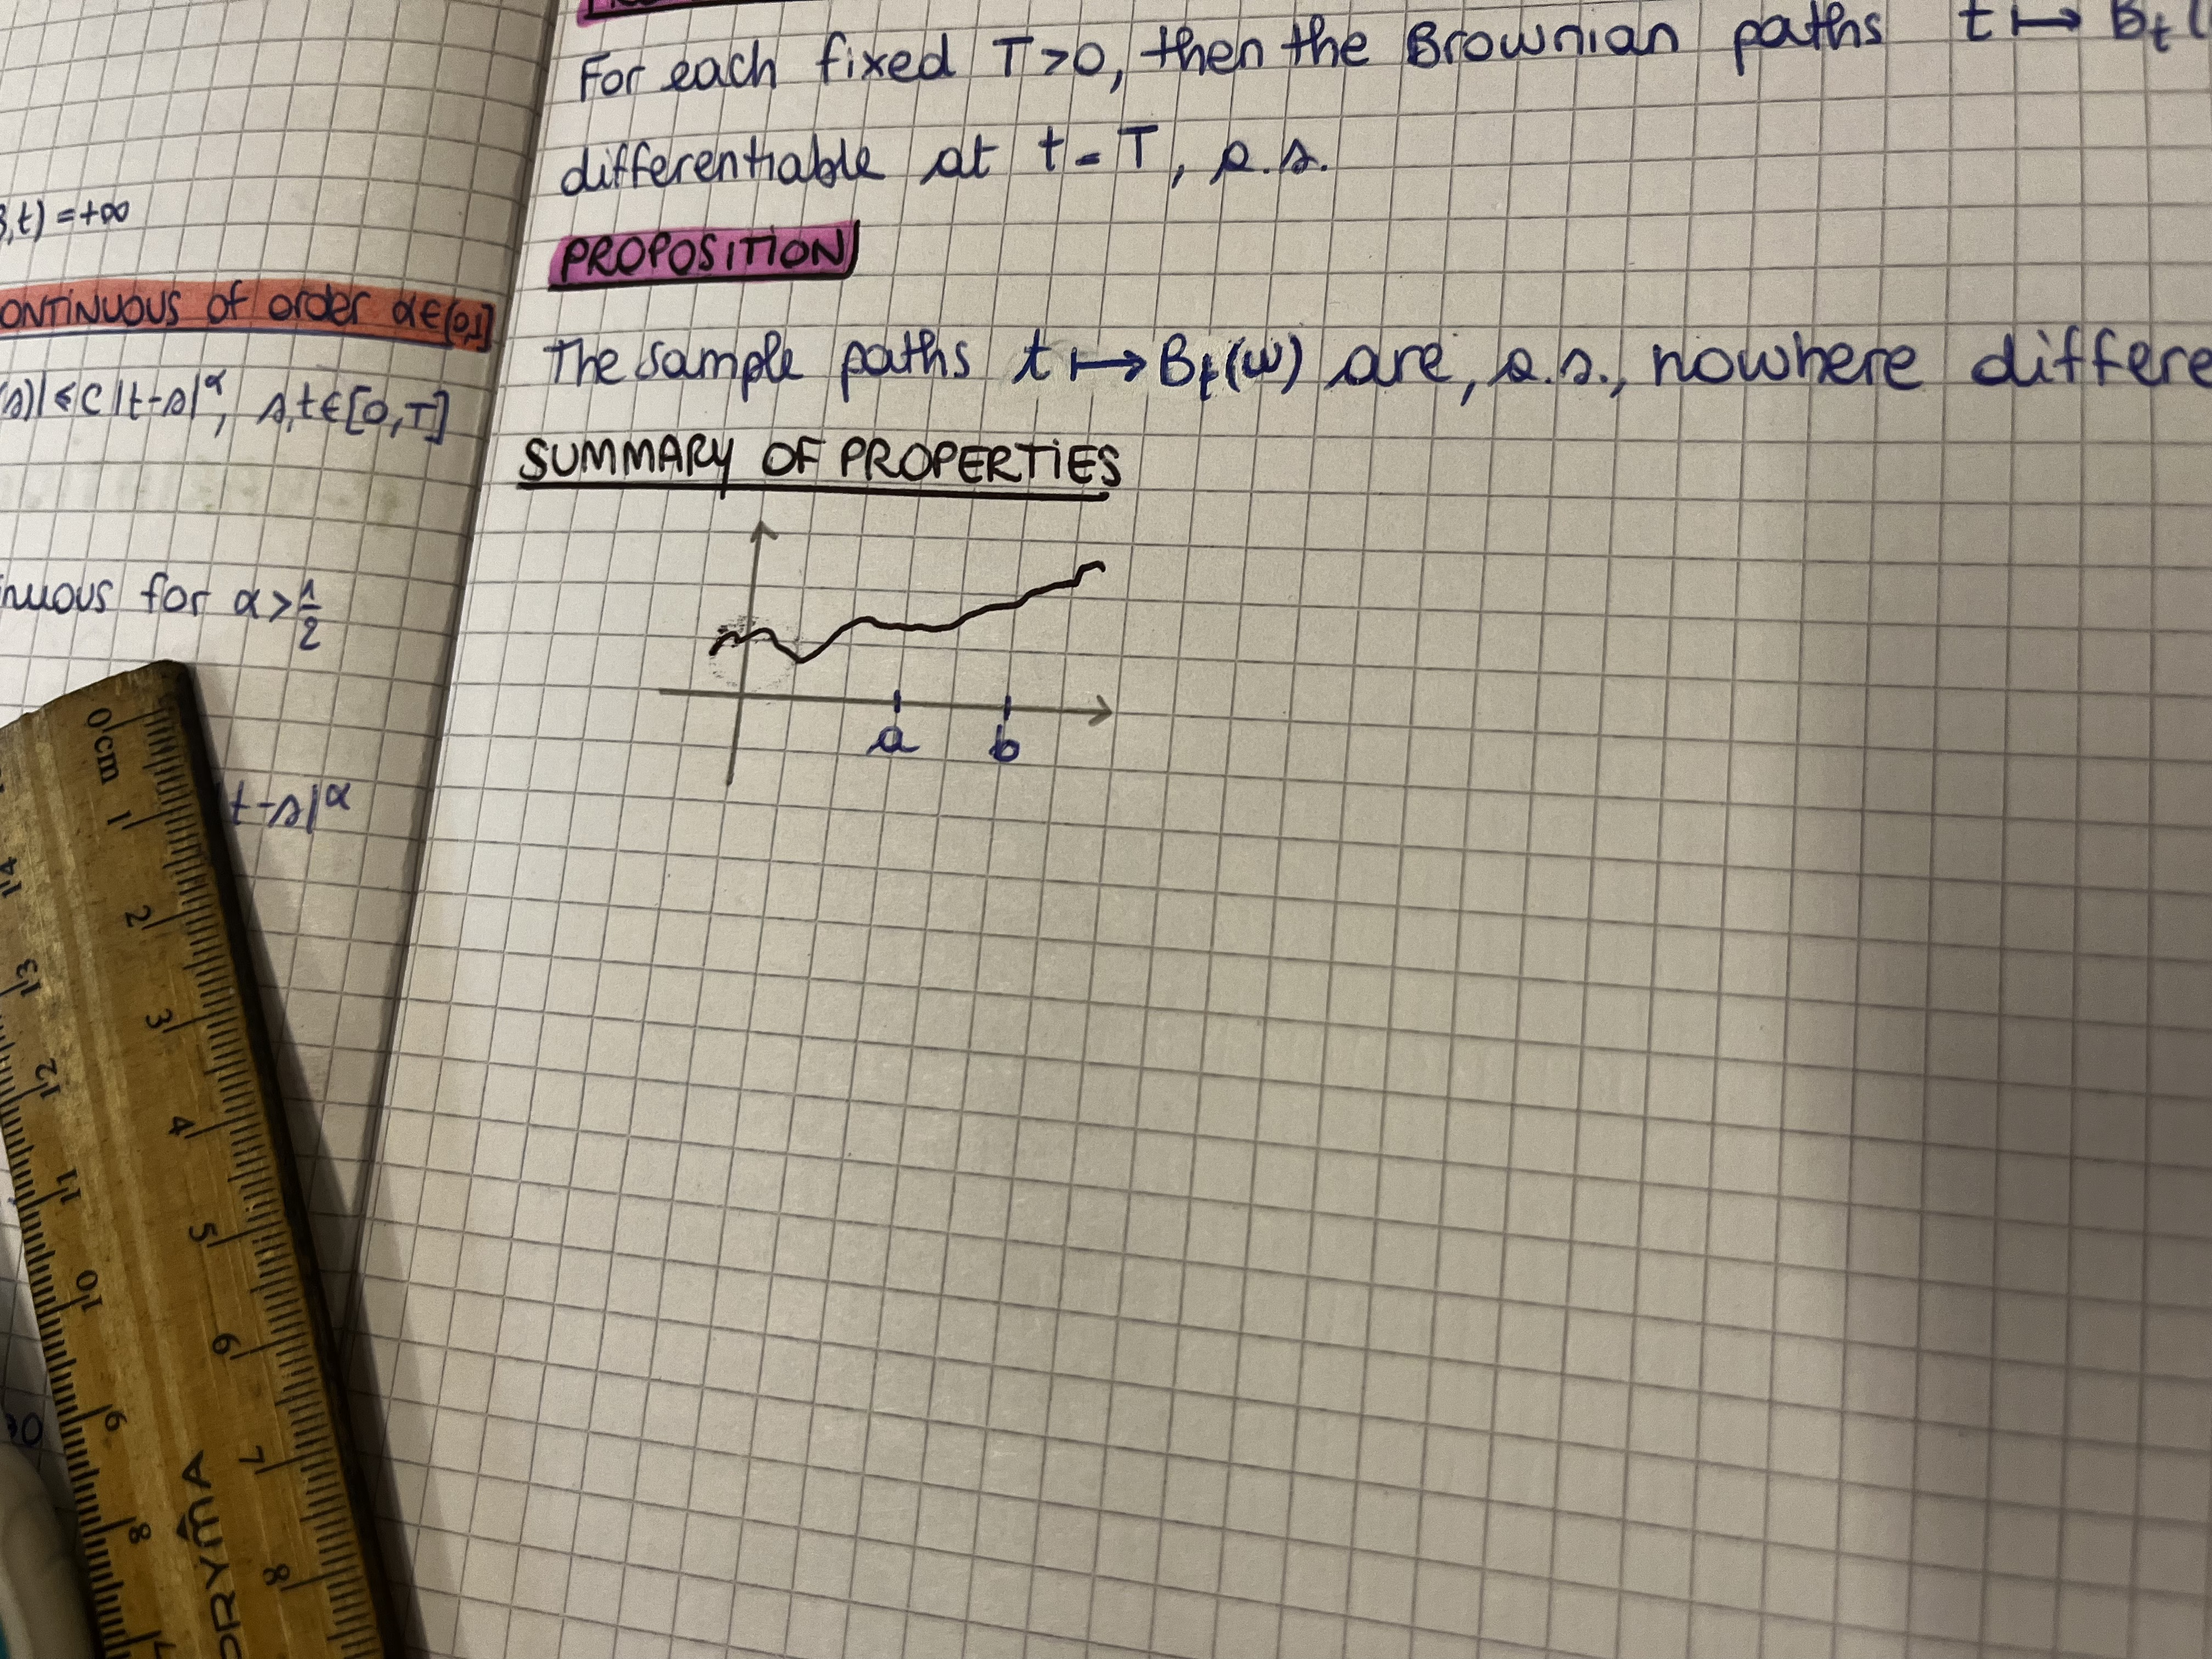
\includegraphics[width=14cm]{IMG_9589.jpeg}\\ 
    \caption{Non-differentiability of the BM} 
    \label{fig_1}
    \end{center} 
\end{figure} 

\begin{remark}
    In Stochastic Processes course we achieved this result by means of the following steps:
    \begin{itemize}
        \item Differentiability of a function in a point implies that the function itself is Holder continuous of order $\alpha = 1$ in a neighbourhood of the point.
        \item We proved, as above, that the path of a BM is \emph{not} Holder continuous of order $\alpha \geq \frac{1}{2}$ almost surely.
        \item Then, since the Holder continuity does not hold for $\alpha \geq \frac{1}{2}$, it cannot be valid in particular for $\alpha = 1$. Therefore, by the result in the first item, we get that the function (that is, the BM path) is nowhere differentiable. 
    \end{itemize}
\end{remark}
\begin{PropBox}
    \begin{Proposition}
    With probability $1$, there is no interval $[a,b] \subset (0,+\infty)$ where $t \mapsto B_t$ is monotone. 
\end{Proposition}
\end{PropBox}
\begin{remark}
    This is true also in $\mathbb{R}^d$. 
\end{remark}
Regardless of the length of the interval $[a,b]$ we consider, provided that it is finite, we will never find either monotone increasing or monotone decreasing paths. Instead, they will always be oscillating. \\
Moreover, even if the interval we pick has very small length, the distance ran by the
function will always be infinite. Indeed, from Stochastic Processes course, we know that the oscillations of the BM are infinite and of small amplitude. \\
The goal of the lecture is to show that the following approach does not work.
\begin{equation*}
\begin{split}
    d X_t &= b_c(X_t) dt + \sigma_t(X_t)dB_t\\
    X_t -X_0 &= \int_0^t b_s(X_s) ds + \int_0^t \sigma_s(X_s)dB_s\\
    \int_0^t &\sigma_s(X_s(\omega))dB_s(\omega)
\end{split}
\end{equation*}

\chapter{Stochastic Integration [Professor Toaldo]}
First of all, we recall the main concepts of the \emph{Riemann integration}, which is our starting point. \\
Consider an interval $I=[a,b]$ and imagine we want to integrate a function $f: [a,b] \to \mathbb{R}$ on this interval. Then we consider a partition of the interval 
\begin{equation*}
\begin{split}
     \Pi_n &:= \{a = x_0 < x_1 < \ldots < x_n = b\}\\
    \sum_{j=0}^{n-1} &f(\xi_j) (x_{j+1} - x_j) \quad \xi_j \in [x_j, x_{j+1}]
\end{split}
\end{equation*}

If the limit of the previous sum exists and it equals a constant $C$, then when the mesh of the partition decreases to $0$
\begin{equation*}
    |\Pi_n| \rightarrow 0 
\end{equation*}
\begin{equation}
    \int_a^b f(t) dt:= c
\end{equation}
\begin{remark}
    According to the Riemann integration, for $\int_a^b f(t) dt$ to exist, the function must be \textbf{continuous}, that is $f \in \mathcal{C}([a,b])$. This is a \emph{sufficient} condition. 
\end{remark}
If we are interested in the integration of a function against the increments of another one, we extend the Riemann integral to the \emph{Riemann-Stieltjes} integral:
\begin{equation*}
    \int_a^b f(t)dg(t)
\end{equation*}
We take the sum
\begin{equation*}
    \sum_{j=0}^{n-1} f(\xi_j)(g(x_{j+1})-g(x_j)) \hspace{1 cm} \xi_j \in [x_j, x_{j+1}]
\end{equation*}
letting the mesh of the partition go to $0$
\begin{equation*}
    |\Pi_n|\ra 0
\end{equation*}
The two conditions for the Stieltjes integral of $f$ to exist are:
\begin{itemize}
    \item $f$ and $g$ without any discontinuity at the same point $x$ $\rightarrow$ \emph{necessary} condition.
    \item $f$ is continuous and $g$ is of bounded variation, $\rightarrow$ \emph{sufficient}, but \emph{not} necessary condition.
\end{itemize}
\begin{equation}
    \int_0^t \sigma_s(X_s) dB_s \stackrel{Riemann-Stieltjes} = ?
\end{equation}
We are not sure that this integral actually exists. 

If we want to use the notion of integral to integrate along the trajectory we need this integral to cover at least all the continuous functions. Therefore, it's reasonable to require that the integral we are defining 
exists for any $f \in \mathcal{C}([0,T])$.
\begin{equation*}
    \int_0^T f(s) dB_s
\end{equation*}
The problem is given by the following result 
\begin{PropBox}
    \begin{Proposition}
    Let $\alpha:[a,b]\to \mR$ and denote 
    \begin{equation*}
        I(f):= \int_a^bf(t)d\alpha(t)
    \end{equation*}
    If this integral exists as a Riemann-Stieltjes integral for all $f \in \mathcal{C}([a,b])$, then $\alpha$ is of bounded variation, that is:
    \begin{equation*}
    ||\alpha||_{TV} = \sup_{\Pi} \sum_{t_i \in \Pi} |\alpha(t_i)-\alpha(t_{i-1})| < + \infty
\end{equation*}
\end{Proposition}
\end{PropBox}
If we want to use RS integral as a notion to integrate BM, then this is basically hopeless. That's because if we want the integral to cover all the continuous functions over compact intervals, the function must be of bounded variation. The problem is that BM \emph{is not} of bounded variation and so we cannot apply this notion of integral. Therefore, we must define a new kind of integration object to be able to integrate the BM. \\
The Riemann-Stieltjes integral exists, but not for all the continuous functions. \\
For example, the sum does not converge considering the following integral:
\begin{equation*}
    \int_0^t B_s dB_s
\end{equation*}
What's the solution? We must consider all the trajectories of the BM. 
    \begin{PropBox}
        \begin{remark}
        \textbf{Banach-Steinhaus.} Let $(X, ||\cdot||_X)$ and $(Y, ||\cdot||_Y)$ be Banach spaces and let $I$ be any index set. For each $i\in I$, let $S_i: X \to Y$ be a continuous linear map. If 
        \begin{equation*}
            \sup_{i \in I} ||S_i(x)||_Y < \infty \hspace{1 cm} x \in X
        \end{equation*}
    then 
    \begin{equation*}
         \sup_{i \in I} \underbrace{ \sup_{||x||_X \leq 1} ||S_i(x)||_Y < \infty }_{\text{operator norm}}
    \end{equation*}
    \end{remark}
    \end{PropBox}
    We are now going to use this theorem to prove the previous proposition. 
    \begin{proof}
    Consider 
    \begin{itemize}
        \item $X = \mathcal{C}([a,b]), \quad || \cdot || _{\infty}$ as norm 
        \item $Y = \mathbb{R}$
        \item $I$: family of all finite partitions of $[a,b]$, $\Pi = \{a = t_0 < \ldots < t_n = b\}, n \in \mathbb{N}$. 
    \end{itemize}
    Now, let $\Pi \in I$ and define
    \begin{equation*}
       S_\Pi(f) := \sum_{i=1}^n f(t_i) (\alpha(t_i)-\alpha(t_{i-1})) \hspace{0,5 cm} f \in C[a,b]
    \end{equation*}
    Fixing any partition, it is clear that $f \mapsto S_\Pi(f)$ is a linear map. We can therefore apply Banach - Steinhaus theorem:
    \begin{align*}
        |S_\Pi(f)| &\stackrel{(*)}\leq ||f||_{\infty} \sum_{i=1}^n |\alpha(t_i)-\alpha(t_{i-1})| \\ 
        &= C_{\Pi, \alpha} ||f||_{\infty}
    \end{align*}
    where $(*)$ is given by the fact that $f$ is bounded, being continuous over a compact interval. \\
    Therefore, $S_\Pi$ is a bounded (hence continuous) linear map.\\
    Since 
    \begin{equation}
    \label{condition}
        S_\Pi(f) \rightarrow \int_a^b f(t) d\alpha(t) \quad \forall f \in \mathcal{C}([a,b])
    \end{equation}
    as $|\Pi| \rightarrow 0$, then 
    \begin{equation*}
       \sup_\Pi |S_\Pi(f)| < + \infty
    \end{equation*}
    Indeed, if by contradiction the supremum was infinite, then it would be so over a set of partitions with mesh going to $0$. Nevertheless, we will never reach infinity because of the assumption about convergence in \eqref{condition}.\\
    Therefore, by Banach-Steinhaus,
    \begin{equation*}
        \sup_\Pi \sup_{||f||_\infty \leq 1} |S_\Pi(f)|<+ \infty
    \end{equation*}
    Now, we want to use this to prove that the function $\alpha$ must be of bounded variation, that is 
    \begin{equation*}
        ||\alpha||_{TV} < +\infty
    \end{equation*}
    This is true since
    \begin{equation*}
    \begin{split}
        ||\alpha||_{TV} &= \sup_\Pi \sum_{i=1}^n |\alpha(t_i)- \alpha(t_{i-1})|\\
        &= \sup_\Pi S_\Pi(f_\Pi)\\
        & \stackrel{(*)}\leq \sup_\Pi \sup_{||f||_\infty \leq 1} |S_\Pi(f)| < \infty
    \end{split}
    \end{equation*}
     \begin{figure}
\begin{center} 
  % Requires \usepackage{graphicx} 
  \includegraphics[width=14cm]{IMG_9591.jpeg}\\ 
  \caption{$f$ piecewise linear}
  \label{fig_2}
\end{center} 
\end{figure} 
    The last inequality $(*)$ is justified as follows. We consider $f$ piecewise linear (as in Figure \ref{fig_2}) with
    \begin{align*}
        f_\Pi(t_i) &= \text{sign}(\alpha(t_i) - \alpha(t_{i-1}))\\
        & \stackrel{ \text{R.S.}}\leq \sup_{\Pi} \sup_{||f||_{\infty} \leq 1} |S_\Pi(f)| < +\infty
    \end{align*} 
\end{proof}
\begin{remark}
    In practice, what we understand is that - since the Brownian paths are almost surely not of bounded variation - they cannot be defined as a RS integral $\int_0^T f(t) dB_t$ if the class of admissible integrands contains all continuous functions $f$ on $[0,T]$.
\end{remark}
To solve the problem, we change the kind of convergence.  
\chapter{Ito Integral [Professor Toaldo]}
\begin{equation*}
    \lim_{|\Pi| \ra 0} \sum_{t_i \in \Pi}f(t_i) (B(t_{i+1})-B(t_i))
    \end{equation*}
could be infinite for $f \in \mathcal{C}([a,b])$. In practice, the idea is to modify the convergence considering the $L^2$ limit $L^2 - \lim_{|\Pi| \rightarrow 0}$: we do not consider the BM path by path, but we consider instead the entirety of the trajectories. We are now giving a definition of Lebesgue integral, to move finally on to the Ito integral.
\begin{DefBox}
    \begin{Def}
    Consider a \textbf{positive simple function} $f$, that is 
    \begin{equation*}
        f = \sum a_i \mathbbm{1}_{[t_{i-1}, t_i)}
    \end{equation*}
and its \textbf{integral} over the interval $[a,b]$:
    \begin{equation*}
        \int_a^b f(t)dt=\sum_{i_1}^n a_i|t_i -t_{i-1}| \hspace{2 cm} t_i \in \Pi
    \end{equation*}
    We know that, for every positive simple function (piecewise constant), there exists a sequence of functions $f_n \uparrow f$. Therefore
    \begin{equation*}
        \int_a^b f dt  = \lim_{n \rightarrow +\infty}\int_a^b f_n dt
    \end{equation*}
    Considering the decomposition involving positive and negative parts of the function
    \begin{equation*}
        f = f^+ - f^-
    \end{equation*}
    we get 
    \begin{equation*}
        \int_a^b f dt = \int_a^b f^+ dt - \int_a^b f^- dt 
    \end{equation*}
\end{Def}
\end{DefBox}
We divide the interval $[a,b]$ into $n$ sub-intervals and look at approximating sums
\begin{equation*}
    S_n = \sum_{j = 1}^n f(B_{s_j}) (B_{t_{j+1}} - B_{t_j}) \quad s_j \in [t_j, t_{j+1}]
\end{equation*}
Since the variation of the BM paths is not bounded, the pointwise limit of $S_n$ does not exist and therefore we cannot use RS definition of integral. \\
However, we are going to see that if we consider $S_n$ as an element of $L^2(\Omega, dP)$, then it \emph{does} have a limit. \\
Unfortunately, even in this setting, the limit will depend on how the point $s_j$ is chosen, unlike the RS case. \\
For this first part of the discussion, we will restrict on $s_j = t_j$, meaning that we will choose the integrand to be adapted to the filtration. 

\begin{DefBox}
    \begin{Def}[Step process]
    Let $[S,T] \subset \mR$ be an interval and let $(\mathcal{F}_t^B)_{t \geq 0}$ be the natural filtration of BM. We call $(f_t)_{t \in [S,T]}$ a \textbf{random step process} if there is a partition $S=t_0 < t_1 < \dots < t_n =T$ and random variables $\eta_0, \eta_1, \ldots, \eta_{n-1} \in L^2(\Omega, dP)$ such that $\eta_j$ are $\mathcal{F}_{t_j}^B$-adapted and 
    \begin{equation*}
        f_t = \sum_{j=0}^ {n-1} \eta_j \mathbbm{1}_{[t_j, t_{j+1}]}(t)
    \end{equation*}
    meaning that $f_t$ is a simple function. 
\end{Def}
\end{DefBox}
\begin{DefBox}
    \begin{Def}
    We denote by 
    \begin{equation*}
        M^2_{\text{step}}([S,T])
    \end{equation*}
    the class of random step processes.
\end{Def}
\end{DefBox}
\begin{remark}
    In general, a step process is not a Markov process.
\end{remark}
\begin{DefBox}
    \begin{Def}
    Let $f_t \in M^2_{\text{step}} ([S,T])$. We define the \textbf{Ito integral of $f_t$} with respect to the BM by
    \begin{align*}
        I(f)&:=: \int_S^T f_t dB_t \\
       &:= \sum_{j=0}^{n-1} \eta_j (B_{t_j} - B_{t_{j-1}})
    \end{align*}
\end{Def}
\end{DefBox}
The two definitions are equivalent and the latter one shows the similarity to the Lebesgue integral definition.  \\
We remark that the integral is a random variable, not a number, since it depends on $\omega$. 
\begin{PropBox}
    \begin{Proposition}
    For every $f_t \in  M^2_{\text{step}}([S,T]) $ we have 
    \begin{equation*}
        I(f) \in L^2(\Omega, dP)
    \end{equation*}
    that is, $I(f)$ is a random variable in $L^2$.
    Moreover, the $L^2$-norm is:
    \begin{equation*}
        \underbrace{\mathbb{E}[I(f)]^2}_{||I(f)||^2_{L^2(\omega)}} = \underbrace{\mathbb{E}[\int_S^T f_t^2 dt]}_{||f||^2_{L^2(\Omega \times [S,T])}} \quad \text{ called \textbf{Ito isometry}}
    \end{equation*}
    It is called isometry since it is an equality between the norms on two different spaces: the first one concerns a random variable on $\Omega$, while the second one is on $\Omega \times [S,T]$. 
\end{Proposition}
\end{PropBox}
\begin{remark}
    This is true for general processes too.
\end{remark}
\begin{ProofBox}
    \begin{proof}
Denote 
    \begin{equation*}
        \Delta_jB = B_{t_{j+1}} - B_{t_j} \quad \text{ and }  \quad \Delta_j t= t_{j+1} - t_j
    \end{equation*}
    Then,
    \begin{align*}
        [I(f)]^2 &= \Big[\sum_{j=0}^{n-1} \eta_j (B_{t_{j+1}} - B_{t_j})\Big]^2 \\
        &= \sum_{j=0}^{n-1}\sum_{k=0}^{n-1}\eta_j\eta_k \Delta_j B\Delta_k B    \\
        &= \sum_{j=0}^{n-1} \eta_j^2 (\Delta_j B)^2 + 2 \sum_{k>j} \eta_j\eta_k \Delta_j B\Delta_k B 
    \end{align*}
    Now, consider $j < k$ and compute (using Tower Rule and independence of increments)
    \begin{align*}
        \mE [\eta_j \eta_k \Delta_j B \Delta_k B] & \hspace{0 cm } \stackrel{ \text{tower rule}}{=} \mathbb{E} \mathbb{E}[\eta_j \eta_k \Delta_j B \Delta_k B | \mathcal{F}_{t_k}^B] \\
    &\stackrel{\text{conditional determinism}}{=} \eta_j \Delta_j B \eta_k \underbrace{\mE[\Delta_k B| \mathcal{F}_{t_k}^B ]}_{\mathbb{E}[\Delta_k B] = 0} \\
    & \hspace{1,5 cm }= 0\\
    \end{align*}
Taking the expectation:
    \begin{align*}
    \mE[I(f)]^2 &= \mathbb{E}\Big[\sum_{j=0}^{n-1} \eta_j^2(\Delta_j B)^2\Big] +0 \\
    &= \sum_{j=0}^{n-1}\mE \eta_j^2 (\Delta_j B)^2\\
    &= \sum_{j=0}^{n-1}{\mE \underbrace{ \mE [\eta_j^2(\Delta_j B)^2 |\mathcal{F}_{t_j}^B]}_{\mE(\Delta_j B)^2= \Delta_j t}}
    \end{align*}
    since $ \eta_j \in L^2(\Omega, dP)$,  $\mE \eta_j < + \infty$ and so  $\mE [I(f)]^2 < + \infty$. Now, consider that 
    \begin{align*}
        f_t^2 &= \sum_{j = 0}^{n-1} \sum_{k=0}^{n-1} \eta_j \eta_k \mathbbm{1}_{[t_j,t_{j+1})}{(t)} \mathbbm{1}_{[t_k, t_{k+1})}{(t)}\\
        &= \sum_{j = 0}^{n-1} \eta_j^2 \mathbbm{1}_{[t_j, t_{j+1})}{(t)} 
    \end{align*}
    which means that 
    \begin{equation}
    \label{result}
        \mathbb{E}\int_S^T f(t)^2 dt = \sum_{j=0}^{n-1} \mathbb{E}\eta_j^2\Delta_j(t)
    \end{equation}
    Indeed: 
    \begin{equation*}
        \mE \int_S^T f_t^2 dt= \mE \int_S^T \sum_{j = 0}^{n-1} \eta_j^2 \mathbbm{1}_{[t_j, t_{j+1})}^{(t)} dt= \sum_{j = 0}^{n-1} \mE \eta_j^2 \Delta_j(t)
    \end{equation*}
    Using \ref{result} together with 
    \begin{equation*}
        \mathbb{E}I(f)^2 = \sum_{j=0}^{n-1} \mathbb{E}\eta_j^2 \Delta_j t
    \end{equation*}
    proved above we can conclude the proof.
\end{proof}

\end{ProofBox}
\section{Lecture 4}
To define the Ito integral with respect to BM for more general integrals, we are going to approximate integrands by random step processes. To this aim, we introduce the space of random processes as follows. 
\begin{DefBox}
    \begin{Def}
    $M^2(S,T)$ is the class of real valued stochastic processes 
    $f: \mR^+ \times \Omega \to \mR$ such that 
    \begin{itemize}
        \item $(t,\omega) \mapsto f_u(\omega)$ is measurable, for every $u \in [S,T]$ with respect to $([S,u] \times \Omega, \mathcal{B}([S,u]) \otimes \mathcal{F}_u^B)) \to (\mathbb{R}, \mathcal{B}(\mathbb{R}))$. This property is called \textbf{progressive measurability}. 
        \item $\mathbb{E}[\int_S^T f_t^2 dt]< +\infty$ that is, the $L^2$ norm must be finite. 
    \end{itemize}
\end{Def}
\end{DefBox}
What this definition tells us is that $f$ must be a function of the Brownian Motion, measurable with respect to its filtration with respect to $\omega$. The first condition concerns regularity with respect to the Borel $\sigma$-algebra and as a function of time. 

\begin{PropBox}
    \begin{Proposition}
\label{prop_progressive}
    Let $X$ be a right continuous process adapted to $\mathcal{F}_t^B$. Then it is progressively measurable.
\end{Proposition}
\end{PropBox}
\begin{remark}
    $M^2_{\text{ step}}$ is right continuous, therefore it is progressively measurable. 
\end{remark}
Consider the following \\
\textbf{Example} Imagine we want to integrate the process $X$, in particular:
\begin{equation*}
    Y_t = \int_0^t X_s ds \hspace{2 cm} X=(\Omega, \mathcal{F}, \mathcal{F}_t, X_t, \mP)
\end{equation*}
We want to make sure that this integral actually exists and is well-defined on $X$. 
In particular, we wonder whether the mapping $\omega \mapsto Y_t(\omega)$ is a random variable in $\mathcal{F}_t$ or not. \\
We know that if $X$ is progressively measurable, then the map 
\begin{equation}
\label{ex_map}
    (\omega, s) \mapsto X_s(\omega) 
\end{equation}
is $\mathcal{F}_t \otimes \mathcal{B}([0,t])$-measurable. By Fubini's theorem the map
\begin{equation*}
    \omega \mapsto \int_0^t X_s(\omega) ds 
\end{equation*}
is $\mathcal{F}_t$-measurable. It follows that $Y$ is adapted to $\mathcal{F}_t$ and also progressively measurable, since it is continuous. We report hereby the Fubini's theorem statement. 
\begin{ThBox}
    \begin{Th}[\textbf{Fubini's Theorem}]
    Let $\mu_1$ and $\mu_2$ be measures on $(E_1, \mathcal{E}_1)$ and $(E_2, \mathcal{E}_2)$ measurable spaces and $f: E_1 \times E_2 \to \mR$ measurable with respect to $\mathcal{E}_1 \otimes \mathcal{E}_2$. Suppose that at least one of the following is true 
    \begin{itemize}
        \item $f$ is integrable with respect to $\mu_1 \otimes \mu_2$
        \item $f$ is positive 
    \end{itemize}
    Then it is true that 
    \begin{itemize}
        \item the following functions are measurable with respect to $\mathcal{E}_1$ and $\mathcal{E}_2$ respectively. 
        \begin{equation*}
            \begin{split}
                x_1 \mapsto \int f(x_1,z) &\mu_2(dz) \hspace{2 cm} \in \mathcal{E}_1\\
                x_2 \mapsto \int f(z, x_2) &\mu_1(dz) \hspace{2 cm} \in \mathcal{E}_2
            \end{split}
        \end{equation*}
        \item \begin{align*}
            \int _{E_1 \times E_2} f d\mu_1 \otimes d\mu_2 &= \int \mu(dx_1) \int f(x_1, x_2) \mu(dx_2) \\
            &= \int \mu(dx_2) \int f(x_1, x_2) \mu(dx_1)
        \end{align*}
    \end{itemize}
\end{Th}
\end{ThBox}
Now, recall the equation we stated in the previous lectures:
\begin{equation*}
    dX_t = \underbrace{b_t(X_t) dt}_{\text{Riemann int}} + \underbrace{\sigma_t(X_t) dB_t }_{\text{Itô int}} 
\end{equation*}
A corollary of Proposition \ref{prop_progressive} is the following
\begin{Cor}
    $M^2_{\text{step}}([S,T]) \subset M^2([S,T])$ 
\end{Cor}
Indeed, $M^2_{\text{step}}$ processes are right continuous and therefore progressively measurable too. \\
In practice, we are enlarging the class of functions that can be integrated since the functions are not required to be step processes anymore. The usage of step processes is crucial since they are dense in $M^2$.

\begin{Lemma}
\label{lemma_2}
    Suppose $(f_t)_{t \in [S,T]} \in M^2(S,T)$. Then, there exists a sequence $(\phi^n)_{n \in \mathbb{N}} \subset M^2_{\text{step}}([S,T])$ such that 
    \begin{equation*}
        \mathbb{E}\big[\int_S^T |f_t(\omega) - \phi_t^ n(\omega)|^2 dt\big] \ra 0, \quad \text{for } n \ra +\infty
    \end{equation*}
\end{Lemma}
This can be written as 
\begin{equation*}
    \mathbb{E}[\int_S^T |f_t - \phi_t^ n|^2 dt] = ||f_t - \phi_t||_{L^2(\Omega \times [S,T])} \ra 0 \hspace{ 2 cm} n \ra + \infty
\end{equation*}


This lemma tells us that whenever we pick a random process that we want to integrate, then we can identify a class of $L^2$ step processes converging to it. It's the same as what happens with Lebesgue integral, in which there exists a sequence of positive functions converging to the integrated function. The difference here is that the sequence converges to the function $f$ not point-wise but in $L^2$.  

\begin{ProofBox}
    \begin{proof}[Sketch of the proof]
We prove roughly the statement proceeding in $4$ steps. \\
   \emph{Step 1}: consider $g_t \in M^2(S,T)$ bounded and such that $t \to g_t (\omega)$  is continuous, for every $\omega \in \Omega $.
   \begin{equation*}
   \Phi_t^n:= \sum_j g_{t_j}(\omega) \mathbbm{1}_{[t_j, t_{j+1})}{(t)}
   \end{equation*}
   \begin{equation*}
       L^2(\Omega \times [S,T])- \lim_{n \ra \infty} \phi_t^n = g_t 
   \end{equation*}
   In this step, we prove the Lemma under the hypothesis of \emph{bounded and continuous} functions. \\
   \emph{Step 2}: $h_t \in M^2(S,T)$ bounded. Let $\psi^n(s)$ non-negative, continuous and supported on $K \subset [-\frac{1}{n}, 0] $ and such that 
   \begin{equation*}
       \int \psi^n(s) = 1
   \end{equation*}
   Then
   \begin{equation*}
       g_t(\omega)= \int_0^t \psi^n(s_t) h_s(\omega) ds 
   \end{equation*}
   is continuous and bounded.
   \begin{equation*}
       L^2(\Omega \times [S,T])- \lim_{n \ra +\infty} g^n_t(\omega) = h_t
   \end{equation*}
   In this step we use Step $1$ implicitly to prove the entire Lemma whenever $h_t$ is \emph{only bounded} and not continuous. \\
   Step 3: Let $f \in M^2(S,T)$
   \begin{equation*}
   h_t^n(\omega) = 
       \begin{cases}
         - n & f_t(\omega) < -n \\
         f_t(\omega) & -n < f_t(\omega) < n\\
         n & f_t(\omega) > n
       \end{cases}
   \end{equation*}
   is bounded. 
   \begin{equation*}
       L^2(\Omega \times [S,T])-\lim_{n \rightarrow +\infty} h_t^n(\omega) = f_t
   \end{equation*}
   In this step we get rid of the hypothesis about boundedness too, to prove the entire Lemma for functions in $M^2$. \\
   Finally, by the previous steps, we conclude that we can always find a step process satisfying the statement. 
\end{proof}
\end{ProofBox}
Here, similarly of Lebesgue integration, we remove each time an assumption up to generality. This time, though, we work in the $L^2$ space. \\
Now, putting together the density of $M^2_{\text{step}}$ in $M^2$ and the Ito Isometry, what we get is the definition of Ito integral on $M^2$. \\
Recall that density means that whenever we pick a process in $L^2$ we can find a sequence of step processes converging to it. 
\begin{equation*}
    (\phi_t^n)_{n \in \mathbb{N}} \subset M^2_{\text{step}}, f_t \in M^2 \quad \text{such that} \quad \phi_t^n \rightarrow f_t \quad L^2(\Omega \times [S,T])
\end{equation*}
We know that we can define Ito integral for any $L^2$ step process \\

Now, the aim is to prove that the sequence of integrands is convergent in $L^2$ to a limit, which will be exactly the Ito integral. 
\begin{equation*}
    I(f):= L^2-\lim_n \int_S^T \phi_t^n dB_t
\end{equation*}
The best way to prove it is to show it is a Cauchy sequence. 
Immagine we want to define 
\[
I(f) := \lim_{n \to \infty} \int_S^T \phi_n(t) \, dB_t.
\]
We notice two problems with this definition: 
\begin{itemize}
    \item first of all we are not sure about the convergence of $\phi_n(t) \, dB_t$
    \item second of all, even if it converges, we have no certainty about the meaningfulness of this definition
\end{itemize}  
The answer to the second question is negative, in fact we need a definition of $L^2$-limit.\\
For the convergence problem we check that the previous Lemma combined with the Ito isometry implies that 
\begin{equation*}
    (\int_S^T \phi_t^n dB_t)_{n \in \mathbb{N}}
\end{equation*}
is a $L^2(\Omega)$ - Cauchy sequence. This way, $\int_S^T \phi_t^ndB_t$ must converge to a random variable in $L^2(\Omega)$ as $n \rightarrow +\infty$. \\
To prove it, we use the following 
\begin{Lemma}
    The Ito integral on $M^2_{\text{step}}$ is linear, that is 
    \begin{equation}
        I(\alpha_1 f^1+\alpha_2 f^2) = \alpha_1 I(f^1) + \alpha_2I(f^2)
    \end{equation}
\end{Lemma}
\begin{ProofBox}
    \begin{proof}
    Recall the definition of Ito integral of $f$ with respect to the BM:
    \begin{equation*}
        I(f) := \int_S^T f_t dB_t = \sum_{j=0}^{n-1} \eta_j (B_{t_j} - B_{t_{j-1}})
    \end{equation*}
    Then,
    \begin{align*}
         I(\alpha_1 f^1+\alpha_2 f^2) &=  \int_S^T (\alpha_1 f^1+\alpha_2 f^2) dB_t \\
         &= \int_S^T \alpha_1f^1 dB_t + \int_S^T \alpha_2 f^2 dB_t \\
         &= \alpha_1\int_S^T f^1 dB_t + \alpha_2\int_S^T f^2 dB_t \\
         &= \alpha_1 I(f^1) + \alpha_2I(f^2)
    \end{align*}
    by the linearity property of the integral. 
\end{proof}

\end{ProofBox}
Now we can prove that $(\int_S^T \phi_t^n dB_t)_{n \in \mathbb{N}}$ is in fact an $L^2(\Omega)$ - Cauchy sequence. 
\begin{ProofBox}
    \begin{proof}
We want to show that $\mE \big( \int_S^T \phi_t^n dB_t - \int_S^T \phi_t^m dB_t\big)^2 \xrightarrow{n,m \rightarrow + \infty} 0$.
\begin{align*}
        \mE \big( \int_S^T \phi_t^n dB_t - \int_S^T \phi_t^m dB_t\big)^2 &\stackrel{\text{linearity}}= \mE \big( \int_S^T (\phi_t^n - \phi_t^m) dB_t\big)^2 \\
        &\stackrel{\text{Ito isometry}} = \mathbb{E}\big( \int_S^T (\phi_t^n - \phi_t^m)^2 dB_t\big) \\
        &= || \phi_t^n - \phi_t^m ||_{L^2(\Omega \times [S,T], dt \times dt} \xrightarrow{n,m}0
\end{align*}
since by Lemma \ref{lemma_2}
\begin{equation*}
    ||\phi_t^n - f_t ||_{L^2(\Omega \times [S,T])}  \xrightarrow{n,m}0 
\end{equation*}
\end{proof}
\end{ProofBox}
\begin{DefBox}
    \begin{Def}
    Let $(f_t)_{t \in [S,T]} \in M^2 (S,T)$ and $(\phi^n)_{n \in \mathbb{N}} \subset M^2_{\text{step}}(S,T)$ such that 
    \begin{equation*}
        \phi^n \rightarrow f \quad \text{that is} \quad \lim_{n \rightarrow \infty} \mE\Big[\int_S^T |f_t - \phi_t^n | ^2 dt \Big] = 0
    \end{equation*}
     in $L^2(\Omega \times [S,T])$.\\
     Then, we define the \textbf{Ito integral of $(f_t)_{t \in [S,T]}$ on $[S,T]$} by
     \begin{align*}
         I(f) &:= \int_S^T f_t dB_t \\
         &:= L^2(\Omega)-\lim\int_S^T \phi^n_t dB_t
     \end{align*}
\end{Def}
\end{DefBox}
\begin{remark}
    Notice that the Ito integral is well-defined for any $n$.\\
    Moreover, note also that the limit definition of $\int_S^T f_t dB_t$ is independent of che choice of the random step process.
\end{remark}
It is important to remark also the difference between the two spaces involving $L^2$: the first one is $L^2(\Omega)$ while the second one is $L^2(\Omega \times [S,T])$, which is the product space. The first one is the domain of definition of the Ito integral, while the second one contains all the functions which are integrated according to Ito integral definition.\\

\chapter{Properties of the Ito Integral [Professor Toaldo]}
Now, let us prove the following 
\begin{PropBox}
    \begin{Proposition}[Ito Isometry for $M^2$ processes]
    If $f=(f_t)_{t \in [S,T]} \in M^2(S,T)$, then
    \begin{equation*}
        \mathbb{E}\Big[\int_S^T f_s dB_s\Big]^2 = \mathbb{E}[\int_S^T f_s^2 ds]
    \end{equation*}
    which is equivalent to say
    \begin{equation}
        ||I(f)||_{L^2(\Omega)} = ||f_s||_{L^2(\Omega \times [S,T])}
    \end{equation}
\end{Proposition}
\end{PropBox}
\begin{ProofBox}
    \begin{proof}
    \begin{align*}
        \mathbb{E}\Big[\int_S^T f_s dB_s\Big]^2 &\stackrel{(*)}= \lim_n \mathbb{E}\Big[\int_S^T \phi_s^n dB_s\Big]^2 \\
        &\stackrel{(-)}= \lim_n \mathbb{E} \int_S^T (\phi_s^n)^2 ds = ||\phi_s^n||_{L^2(\Omega \times [S,T])}\\
        &\stackrel{(**)}= \mE \int_S^T f(s)^2 ds
    \end{align*}
    where 
    \begin{itemize}
        \item $(*)$ follows from 
        \begin{equation*}
            \int_S^T f(s)dB_s = L^2 - \lim \int_S^T \phi_s^n dB_s
        \end{equation*}
        \item $(-)$ derives from the Ito Isometry for step processes
        \item $(**)$ is due to the fact that $\phi_s^n \rightarrow f_s$ in $L^2(\Omega \times [S,T], dP \times dt)$
    \end{itemize}
    \emph{Principle}: if the sequence of functions in $L^2$ converges to the function $f$, then also their respective $L^2$ norms are going to converge one to the other.
\end{proof}
\end{ProofBox}
\begin{remark}
    Recall that the Ito integral is not a path-wise integral. It is instead an $L^2$-limit, therefore it's a random variable. 
\end{remark}

The point now is that when we work with the SDE
\begin{equation*}
    dX_t = \underbrace{b_t(X_t) dt}_{\text{Riemann int}} + \underbrace{\sigma_t(X_t) dB_t }_{\text{Itô int}} 
\end{equation*}
we see that it is not valid FOR EVERY $t \in [0,T]$. \\
A SDE is an equation with a Riemann integral and an Ito integral and the aim is to find $X_t $ satisfying the equation almost surely for any $t$ in the interval. \\
We do not want only
\begin{equation*}
    \int_0^t f_s dB_s
\end{equation*}
but we want 
\begin{equation*}
(\int_0^t f_s dB_s)_{t \in [0,T]} = (f_t)_{t \in [0,T]}
\end{equation*}

In particular, through Ito integral we can define a stochastic process (the one indicated above). We want to study the properties of this process, like continuity, adaptedness with respect to the natural filtration of the BM, being a martingale, a Markov process and so on. \\
Now, let us state some important remarks that we will use for this purpose. \\
Consider $f \in M^2([S,T])$. Then, the restriction of $f$ on $[S,t], S \leq t \leq T$ is also $M^2$ and we can work with the real valued process
\begin{equation*}
    I_t=\int_S^t f_s dB_s
\end{equation*}
Clearly 
\begin{itemize}
    \item if $t > s > S$, 
    \begin{align*}
        I_t - I_s &= \int_0^t f_u dB_u - \int_0^s f_u dB_u \\
        &= \lim(\int_S^t f_u^n dB_u - \int_S^s f_u^n dB_u) \\
        &= \lim \int_s^t f_u^n dB_u \\
        &= \int_s^t f_u dB_u
    \end{align*}
    \item $I_t \in \mathcal{F}_t^B$, i.e. it is $\mathcal{F}_t^B$-measurable. \\
    Indeed, since $f^n$ approximates $f$, then $I_t^n = \int_S^t f_s^n dB_s$ approximates $I_t$, that is $I_t^n \rightarrow I_t$ in $L^2$. By definition, $I_t^n$ is $\mathcal{F}_t^B$-measurable. \\
    The convergence in $L^2$ implies the almost sure convergence of a sub-sequence, so $I_t^n \rightarrow I_t$ in $L^2$ implies $I_t^{n_k} \rightarrow I_t$ in $L^2$ almost surely, as $k \rightarrow +\infty$. 
    \begin{equation*}
        \exists \Omega_0: \lim_{k \rightarrow +\infty} I_t^{n_k}(\omega) = I_t(\omega) \quad \forall \omega \in \Omega_0
    \end{equation*}
    Then, it is measurable on $\mathcal{F}_t$ since it is the pointwise limit of a measurable sequence of functions and modifying a random variable on a negligible set still produces a random variable on $\mathcal{F}_t$. \\
    In other words, $I_t$ is a linear combination of functions which are measurable with respect to the natural filtration (BM increments and random variables measurable with respect to it). 
    \item Another obvious property to wonder about is the continuity with respect to $t$.\\
    Notice that if $f_t \in M^2_{\text{step}} [S,T]$, we are considering a finite sum of functions which are continuous
    \begin{equation*}
        f_t = \sum_{i=0}^{n-1} f_i \mathbbm{1}_{[t_i,t_{i+1}]}(t)
    \end{equation*}
    Then we can write
    \begin{equation*}
        I_t = \int_S^t f_s dB_s = \sum_{i=0}^{n-1} f_i(B_{t_{i+1} \wedge t} - B_{t_i \wedge t})
    \end{equation*}
    Therefore, it is easy to conclude that $I_t$ is continuous as well. 
\end{itemize}




\section{Lecture 5}
Before moving on to other properties of the Ito integral, let us make a quick recap of the main concepts we have been studying up to now. \\

In summary, if we want to develop a theory to integrate a function against the BM paths, we should ensure that the following integral 
\begin{equation*}
    \int_S^t f_s d F_s 
\end{equation*}
exists as R.S. integral for any $f \in \mathcal{C}[0,t]$, so $B_s$ of bounded variation. Unfortunately this is impossible, therefore we need to develop a whole new theory based on Lebesgue integration. \\
\begin{equation*}
\begin{split}
     \int_S^T f_s dB = \sum_{i=1}^n \eta_i (\omega)(B_{t_{i+1}}(\omega) - B_{t_i}(\omega))\\
    f_s \in M^2_{\text{step}} \hspace{2 cm}
\end{split}  
\end{equation*}
An important aspect to underline is that this integral is random but it actually depends (besides $\eta$) on $\omega$, that is it depends on the path.\\
Recall the statement of Lemma \ref{lemma_2}, through which we proved that 
\begin{equation*}
    \int_S^T \phi_s^n dB_s
\end{equation*}
is a Cauchy sequence on $L^2(\Omega)$.
We defined 
\begin{equation*}
    \int_S^T f_s dB_s := L^2 - \lim_n \int_S^T \phi_s^n dB_s    
\end{equation*}
This integral is not path-wise defined, that is it is not written as follows
\begin{equation*}
    \int_S^T f_s(\omega) dB_s(\omega)
\end{equation*}
since it is defined as a limit of a sequence of random variables which do not depend on it and converge to something in $L^2$.

\begin{equation*}
    \big(\int_S^t f_s dB_s\big)_{t\in [S,T]}
\end{equation*}
This is a random process, since $(f_s)_{s \in [S,T]}$ is a sequence of random variables in $L^2$ and we should determine its properties.\\

So far, we proved that the random process in analysis is $\mathcal{F}_t^B$-measurable and continuous. Now, we want to see whether there is a connection with martingales or not. 

\begin{ThBox}
    \begin{Th}[Martingale Property]
    Let $(f_t)_{t \in [S,T]} \in M^2[S,T]$. Then the process $(I_t)_{t \in [S,T]}$ is a martingale with respect to $\mathcal{F}_t^B$, where $I_t = \int_S^t f_s dB_s$ and $\mathcal{F}_t^B$ is the natural filtration of the BM.
\end{Th}
\end{ThBox}
\begin{proof}
    \begin{itemize}
        \item Adaptdeness: we proved during last lecture that $I_t$ is $\mathcal{F}_t^B$-measurable since both the integrand and the integrator are measurable. 
        \item Integrability: it follows from 
        \begin{equation*}
            (\mE|I_t|^2) \leq \mE I^2_t = \mE\int_S^t f_s^2 dB_s < \infty
        \end{equation*}
        where the inequality follows from Schwarts inequality and in the equality we used Ito isometry. 
        \item Martingale property: we need to check that $\mathbb{E}[I_s|\mathcal{F}_t^B] = I_t, 0 \leq t \leq s$.\\
        Denote 
        \begin{equation*}
            I_t^n:= \int_S^t \phi_r^n dB_r \quad 
            \text{ where } \quad \phi_t^n = \sum_{j=0}^{n-1} f_j^n \mathbbm{1}_{[t_j^n, t_{j+1}^n)}(t)
        \end{equation*} 
        So, $I_t^n$ is an approximating sequence of $I_t$. Therefore,
        \begin{align*}
            \mathbb{E}[I_s^n|\mathcal{F}_t^B] &=\mE [(\int_S^t + \int_t^s)\phi_r^n dB_r| \mathcal{F}_t^B] \\
            &= \underbrace{\int_S^t \phi_r^n dB_r }_{\mathcal{F}_t^B \text{- measurable}} + \underbrace{\mE[\int_t^s \phi_r^n dB_r |\mathcal{F}_t^B]}_{= 0} 
        \end{align*}
        We would like the expectation to equal $0$ in order to prove the Martingale property, from which it would follow that
        \begin{equation*}
            L^2-\lim \mE[I_s^n|\mathcal{F}_t ^B] = L^2-\lim \int_S^t \phi_r^n dB_r
        \end{equation*}
        The left-hand side should be 
        \begin{equation*}
            \mathbb{E}[I_s^n|\mathcal{F}_t^B] = \mE[I_s|\mathcal{F}_t ^B] \quad\text{since  } I_s^n \xrightarrow{L^2} I_s
        \end{equation*}
        Hence,
        \begin{align*}
            \mE\Bigg[\int_t^s \phi_r^n dB_r |\mathcal{F}_t^B\Bigg] &= \mE\Bigg[\int_t^s \sum_{j=0}^{n-1} f_j^n \mathbbm{1}_{[t_j^n, t_{j+1}^n)}(t)dr|\mathcal{F}_t^B\Bigg] \\
            &= \sum_{t \leq t_j^n \leq t_{j+1}^n \leq s} \mE\Bigg[f_j^n (B_{t_{j+1}^n} - B_{t_j^n}) | \mathcal{F}_t^B\Bigg]\\
            &\stackrel{(*)}= \sum_{t \leq t_j^n \leq t_{j+1}^n \leq s} \mE\Bigg[\mE[f_j(B_{t_{j+1}^n}- B_{t_j^n})|\mathcal{F}_{t}^B]|\mathcal{F}_{t_j^n}^B\Bigg]\\
            &= \sum_{t \leq t_j^n \leq t_{j+1}^n \leq s} \mE\Bigg[\mE[f_j(B_{t_{j+1}^n}- B_{t_j^n})|\mathcal{F}_{t_j^n}^B]|\mathcal{F}_{t}^B\Bigg]\\
            &\stackrel{(-)}= \sum_{t \leq t_j^n \leq t_{j+1}^n \leq s} \mE\Bigg[f_j\mE[(B_{t_{j+1}^n}- B_{t_j^n})|\mathcal{F}_{t_j^n}^B]|\mathcal{F}_{t}^B\Bigg]\\
            &\stackrel{(**)}= 0
        \end{align*}
        where 
        \begin{itemize}
            \item $(*)$: Tower Rule
            \item $(-)$: $f_j$ goes outside of the conditional expectation by its integrability 
            \item $(**)$: the increments of the BM are independent and have expectation $\mE[B_{t_{j+1}^n}- B_{t_j^n}] = 0$. Moreover, we can remove the conditioning by the independence of the increments.
        \end{itemize}
    \end{itemize}
\end{proof}
An important consequence is the following.
\begin{PropBox}
    \begin{Cor}
        Let $(f_t)_{t \in [S,T]}\in M^2[S,T]$. Then 
        \begin{equation*}
            \mE[\int_S^t f_s dB_s]=0 \quad \forall t \in [S,T]
        \end{equation*}
    \end{Cor}
\end{PropBox}
This is true since, being the Ito integral a martingale, the expectation map $t \ra \mE I_t$ is constant. 
%By choosing $S=T$, the result follows (scritto su note alunni anno scorso ma non chiaro). 
\\

What about continuity of the map $t \mapsto I_t$? It is formalized by the following result. 
\begin{ThBox}
    \begin{Th}
    Let $(f_t)_{t \in [S,T]}\in M^2 [S,T]$. Then the random process $(I_t)_{t \in [S,T]}$, $I_t = \int_S^t f_s dB_s$ has a continuous version $(\tilde{I}_t)_{t \in [S,T]}$
    This implies that $\Tilde{I}_t(\omega)$ is continuous $\mathbb{P}$-a.s. and
    \begin{equation*}
        \mathbb{P}(\Tilde{I}_t = I_t) = 1 \quad \forall t \in [S,T]
    \end{equation*}
\end{Th}
\end{ThBox}

\begin{proof}
We consider a sequence of step processes converging to $f$ in $L^2$: 
    $(\phi_t^n)_{n \in \mathbb{N}}\subset M^2_{step}[S,T]$ s.t $\phi^n_t \ra f$ in $L^2(\Omega \times [S,T]) \iff \mE[\int_S^t |f_t(\omega) - \phi_t^n(\omega)|^2 dt] \rightarrow 0$ as $n \rightarrow +\infty$. Let 
    \begin{equation*}
        I_t^n= \int_S^t \phi_s^n(\omega) dB_s
    \end{equation*}
    The schema of the proof will be the following:
    \begin{itemize}
        \item prove $I_t$ is continuous
        \item there exists a suitable subsequence $M_k$ such that $(I_t^{M_k})_{k \in \mathbb{N}}$ is a uniform Cauchy sequence, that is  
        \begin{equation}\label{U-C}
        \sup_{S\leq t\leq T}|I_t^{M_k}-I_t^{M_{k+1}}| \xrightarrow{k \rightarrow +\infty} 0 \hspace{0.5 cm} a.s.
        \end{equation}
        This will imply that 
        \begin{equation*}
        I_t^{M_k}\ra \Tilde{I}_t \quad \text{ uniformly }
        \end{equation*}
        and hence the map
        \begin{equation*}
            t \mapsto \Tilde{I}_t
        \end{equation*}
        is continuous by uniform continuity. Moreover, since 
        \begin{equation*}
            I_t^t \xrightarrow{L^2} I_t \quad n \ra \infty
        \end{equation*}
        \begin{equation*}
            \mP(I_t = \Tilde{I}_t)=1 \quad a.s.
        \end{equation*}
        by the uniqueness of the limit (almost sure convergence to the same element on $L^2$). 
        \begin{remark}
        \begin{itemize}
            \item The aim is to achieve a faster convergence, which will be uniform in time.
            \item Uniform convergence preserves the continuity on a probability one set. 
            \item The point is that the set on which this convergence is true could depend on $t$, so we cannot bring the $t$ into the probability parenthesis. This is why we talk about version and not modification, in which we bring the $t$ inside the parenthesis.
        \end{itemize}
        \end{remark}
    \end{itemize}
    Now, 
    \begin{itemize}
        \item The continuity of $I_t^n$ is implies by the definition of Ito integral for step processes.
        \item To prove that \eqref{U-C} holds, recall the Doob's martingale inequality. Let $(X_t)$ be a martingale with continuous paths. hen, for all $p \geq 1, T \geq 0, \lambda \geq 0$
\begin{equation*}
    \mathbb{P}\Big(\sup_{0 \leq t \leq T} |X_t| \geq \lambda \Big) \leq \frac{1}{\lambda^p} \mathbb{E}[|X_T|^p]
\end{equation*}
 Since $I_t^n$ is a martingale with respect to $\mathcal{F}_t ^B$ and also $I_t ^n - I_t ^m$ is a martingale, we can use Doob's martingale inequality to say that 
    \begin{align*}
        \mathbb{P}\Big(\sup_{S \leq t \leq T} |I_t^n - I_t^n| \geq \epsilon \Big) &\leq \frac{1}{\epsilon^2} \mE[I_T^n-I_T^m]^2\\
        & \stackrel{\text{Ito isometry}}= \frac{1}{\epsilon^2} \mE \Bigg[\int_S^T |\phi_s^n - \phi_s^m|^2 ds \Bigg] \xrightarrow{n,m \rightarrow \infty} 0
    \end{align*}
    since $\phi_s^n$ is Cauchy in $L^2(\Omega \times [S,T])$:
    \begin{equation*}
        \phi_s^n \xrightarrow{L^2(\Omega \times [S,T])} f \quad n\rightarrow\infty
    \end{equation*}
    Now, consider  
    \begin{equation*}
        A_k = \{ \omega \in \Omega: \sup_{S \leq t \leq T} |I_t^{n_k} - I_t^{n_{k+1}}| \geq 2^{-k} \}
    \end{equation*}
    We can choose a subsequence $n_k \xrightarrow{k \rightarrow \infty} \infty$ such that $\mathbb{P}(A_k) \leq 2^{-k}$ and then apply Borel-Cantelli Lemma to find out that, since 
    \begin{equation*}
        \sum_k \mathbb{P}(A_k) < \infty
    \end{equation*}
    then
    \begin{equation}
    \label{liminf}
    \begin{split}
        &\mP(\limsup A_k)=0 \quad \implies \quad \mP(\liminf A_k^C)=1 \\
    \end{split}
    \end{equation}
    If $\omega \in \liminf A_k^C$, then for almost every $\omega \in \Omega$ there exists $N(\omega) < +\infty$ such that $ \forall k > N(\omega)$
    \begin{equation*}
        \sup_{S \leq t \leq T} |X_t^{n_k}(\omega) - X_t^{n_{k+1}}(\omega)| \leq 2^{-k}
    \end{equation*}
    As $k \rightarrow +\infty$, this proves the uniform continuity in the $\liminf A^C_k$, but by the probability of the limit inferior in \ref{liminf} the convergence is almost sure. This is where Borel-Cantelli Lemma is used (final implication). 
    \end{itemize}
\end{proof}
From now on we will always consider the continuous version of the integral even if we don't specify this. \\

An important result Professor Toaldo didn't provide during lecture is a sort of converse of the previous result and it states that a "suitable enough" martingale can be represented as an Ito integral. 
\begin{ThBox}
    \begin{Th}
        Let $(M_t)_{t \geq 0}$ be a continuous square integrable martingale. Then, there exists a unique $\mathcal{F}_t^B$-adapted process $(\eta_t)_{t \geq 0}$ such that $\int_o^t \eta_s^2 ds < \infty$ almost surely $\forall t > 0$ and $M_t - M_0 = \int_0^t \eta_s dB_s, t > 0$.
    \end{Th}
\end{ThBox}

We are now going to study other properties, just stating them without proof. \\
\begin{PropBox}
    \begin{Proposition}
    Let $X,Y \in M^2[S,T]$. Then 
    \begin{equation*}
        \mE\Big(\int_S^T X_s dB_s\int_S^T Y_s dB_s \Big) = \int_S^T \mE[X_s Y_s] ds
    \end{equation*}
\end{Proposition}
\end{PropBox}
This is the equivalent version of the Ito isometry, which applied to $X+Y$ and $X-Y$ proves the result. 
\begin{ThBox}
    \begin{Th}[Uniqueness]
    If $(X_t),(Y_t)$ are processes in $M^2[S,T]$, if there exists a set $A$ such that $\mP(A)=1$ and 
    \begin{equation*}
        X_t = Y_t \hspace{1 cm} \forall t \in [S,T], \forall \omega \in A    
    \end{equation*}
    Then
    \begin{equation*}
        \int_S^T X_t dB_t= \int_S^T Y_t dB_t  \hspace{ 1 cm} a.s.
    \end{equation*}
\end{Th}
\end{ThBox}
This is a stronger version of equal integrability. Notice that it's not enough to require that the processes are versions of each other. We need them to have the \emph{same path}, allowing to put $t$ before the $\omega$ (referring to the path).
\begin{ThBox}
    \begin{Th}
    Let $\tau$ be a stopping time with respect to $\mathcal{F}_t ^B$, with $\tau \leq T$. Then if $f \in M^2[0,T]$ also $f_t \mathbbm{1}_{[t < \tau]}$ is in $M^2[0,T]$  and 
    \begin{align*}
        I_\tau:= \int _0^\tau f_s dB_s = \int _0^T f_s \mathbbm{1}_{(s <\tau)} dB_s, \quad a.s.
    \end{align*}
    \end{Th}
\end{ThBox}
So, if we have a process in a time interval and a stopping time with values in this time interval (bounded by $T$), then this theorem tells us something which is not that trivial. \\
If we stop the process given by Ito integral, which is $(I_t)_{t \in [0,T]}$, at the random time $\tau$, then this is exactly the same as integrating $f_s$ against time indicator function in the time interval. \\
So we have a correspondence between the stopped process and the stopped integral. \\
We should prove then that $f_s \mathbbm{1}_{s \leq \tau}$ is integrable in the Ito sense, that is as element of $M^2$. \\ 

Let us state two other properties.
\begin{PropBox}
    \begin{Proposition}[Approximation of Ito integral]
    Let $f \in M^2, (f_n) \subset M^2$ a sequence such that $f_n \rightarrow f$ in $L^2(\Omega \times [S,T])$. Then
    \begin{equation*}
        \int_S^T f_n dB_s \xrightarrow{L^2(\Omega)} \int_S^T f_s dB_s
    \end{equation*}
\end{Proposition}
\end{PropBox}
It is exactly the same statement given for step processes: we are saying that having a sequence converging to a process, both in $M^2$ but not necessarily being step processes, then we still have the convergence of integrals.
\begin{proof}
    \begin{equation*}
        \mE [\int_S^TX_s^n dB_s - \int_S^T X_s dB_s]^2 = \mE \int_S^T[X_s^n -X_s]^2 ds \ra 0
    \end{equation*}
\end{proof}
It is possible to pick a suitable sequence of step processes that approximates some specific $M^2$ process. 
\begin{PropBox}
    \begin{Proposition}
    Let $f(t)$ be in $M^2[0,T]$ and 
    \begin{equation*}
        [0,T] \times [0,T] \mapsto \mE[f(u) - f(v)]^2
    \end{equation*}
    continuous. Then, define 
    \begin{equation*}
        f^{\Delta n}(t) = \sum_j ^ n f(t_{j-1})\mathbbm{1}_{[t_{j-1},t_j]}(t) \hspace{1 cm} t_j \in \Delta n
    \end{equation*}
    it holds 
    \begin{equation*}
    f^{\Delta n}(t) \rightarrow f(t) \quad L^2(\Omega \times [0,T])
    \end{equation*}
\end{Proposition}
\end{PropBox}
\begin{remark}
    In the statement, we write as index $\Delta n$ instead of $n$ on $f$ since what changes is not the value of the function but the interval in the indicator function representing the partition of $[0,T]$. 
\end{remark}
\begin{ProofBox}
    \begin{proof}
    \begin{align*}
         \mE \int_0^T (f(t')- f^{\Delta n}(t'))^2 dt' &\stackrel{\text{by def of }f^{\Delta n}}{=} \mE \sum_{j=1}^n \int_{s_{j-1}}^{s_j}(f(t')- f(s_{j-1}))^2 dt' \\
         &\stackrel{\text{Fubini}}= \sum_{j = 1}^n \int_{s_{j-1}}^{s_j}\mE (f(t')- f(s_{j-1}))^2 dt' \\
         &\leq \sum_{j=1}^n \sup_{(u,v) \in [s_{j-1},{s_j}] \times  [s_{j-1},{s_j}]} \mE (f(u)- f(v))^2 dt'  \\
         &= \sum_{j=1}^n \sup_{(u,v)\in [s_{j-1}, s_j]\times [s_{j-1}, s_j]} \mE(f(u)-f(v))^2 (s_{j}-s_{j-1}) \rightarrow 0
    \end{align*}
    since, letting the mesh of the partition go to $0$ 
    \begin{equation*}
        |\Delta_n| \rightarrow 0
    \end{equation*}
    it holds that 
    \begin{equation*}
        \sup_{(u,v)\in [s_{j-1}, s_j]\times [s_{j-1}, s_j]} \mE(f(u)-f(v))^2 \rightarrow 0
    \end{equation*}
    by uniform continuity. Indeed $f$, the two variables function, is continuous by assumption on a compact interval, therefore by Heine-Cantor theorem it is uniformly continuous too. Moreover, we know that the supremum of a uniformly continuous function goes to $0$. 
\end{proof}
\end{ProofBox}

We can use this approximation to make explicit computations with complex processes. \\



\chapter{Stochastic Calculus [Professor Toaldo]}
\section{Lecture 6}
Up to now, while dealing with the Ito integral definition, the main idea was to start from the SDE 
\begin{equation*}
    dX_t = b_t(X_t) dt + \sigma_t(X_t) dB_t 
\end{equation*}
and find the process function which is solution of the equation. In Stochastic Calculus we use an approach which is basically the converse: we rather start from the process and find the SDE which is solved by the process itself. \\
In other words, we are now going to analyze the stochastic counterpart of the change of variable formula studied in classical analysis: the Ito formula. 
\begin{equation*}
\begin{split}
    dX_t&= b_t(X_t) dt + \sigma_t (X_t) dB_t\\
    X_t -X_0 &= \underbrace{\int_0^t b_s(X_s) ds}_{\text{Riemann int-}} + \underbrace{ \int_0^t \sigma_s (X_s) dB_s}_{\text{Ito int.}}
\end{split}
\end{equation*}
Considering the solution as a function of the BM
\begin{equation*}
    X_t = h(B_t)
\end{equation*}
and taking its derivative
\begin{equation*}
    \frac{d}{dt}h(B_t) = h'(B_t) \frac{d}{dt}B_t
\end{equation*}
we can clearly notice that this is \emph{NOT} possible since the BM is not differentiable! Therefore, the classical calculus chain rule is not applicable because of the BM. \\
Now, we are going to see how to compute entirely the Ito Integral for a couple of processes. This will lead to the conclusion that, since the computation will be too complex, we will be needing a new and easier way of doing it. \\
\textbf{Example}
\begin{equation*}
    X_t= B_t^2 
\end{equation*}
suppose we want to compute the differential of this process 
\begin{equation*}
    dX_t = 2B_t dB_t 
\end{equation*}
In classical calculus using the chain rule we obtain the result written above, but this is a wrong equality since, considering
\begin{equation*}
    B_t^2 = \underbrace{\int ^t_0 2 B_s dB_s }_{\text{Ito}}
\end{equation*}
and taking the expectations, we get the contradiction
\begin{equation*}
    \mE B^2_t = t \quad \mE[\text{ITO}] = 0
\end{equation*}
Therefore, we could try to use another approach considering a partition of $[0,t]$ 
\begin{equation*}
    \Pi_n=\{0 =t_1 < t_2, \dots, t_n\}
\end{equation*} 
such that $|\Pi_n|\ra 0$. Define
\begin{equation*}
    X_t^n:= \sum_{t_k \in \Pi_n} B_{t_k} \mathbbm{1}_{[t_k, t_{k+1})]}(t)
\end{equation*}
\begin{remark}
    Notice that $X^n_t$ is a stopped process, for any $n$.
\end{remark}
Last lecture we proved that if 
\begin{equation*}
    [0,t]\times [0,t]\mapsto \mE [B(u)-B(v)]^2
\end{equation*}
is continuous then 
\begin{equation*}
    X_t^n \ra B_t \hspace{1 cm} \text{in }L^2(\Omega \times [0,t])
\end{equation*}
and 
\begin{equation*}
    \int_0^t X_s^n dB_s \rightarrow \int_0^t B_s dB_s 
\end{equation*}
in $L^2(\Omega)$. \\
Why is this useful? That's because if we write
\begin{equation*}
    \int_0^t B_t dB_t = L^2- \lim_{|\Pi_n| \rightarrow 0} \sum_{t_k \in \Pi_n} B_{t_k} (B_{t_{k+1}} - B_{t_k})
\end{equation*}
Now we want to manipulate the right-hand side to achieve another result. 
\begin{align*}
    &= \frac{1}{2}L^2-\lim_{|\Pi_n|\ra 0}\sum_{t_k \in \Pi_n}\big[(B_{t_{k+1}}^2-B_{t_{k}}^2)-(B_{t_{k+1}}-B_{t_{k}})^2\big ] \\
    &= \frac{1}{2} (B^2_t - \underbrace{B_0^2}_{= 0 \text{  a.s.}}) - \frac{1}{2} \L^2-\lim_{|\Pi_n|\ra 0} \sum_{t_k \in \Pi_n} (B_{t_{k+1}} - B_{t_k})^2\\
    &= \frac{1}{2}B_t^2 -\frac{1}{2} L^2-\lim_{|\Pi_n|\ra 0}\sum_{t_k \in \Pi_n}(B_{t_{k+1}}-B_{t_{k}})^2
\end{align*}
So we get that 
\begin{equation*}
    \int_0^t B_t dB_t = \frac{1}{2} B^2_t - \frac{1}{2} t
\end{equation*}
since 
\begin{equation*}
    L^2-\lim_{|\Pi_n|\ra 0}\sum_{t_k \in \Pi_n}(B_{t_{k+1}}-B_{t_{k}})^2 = t
\end{equation*}
by the quadratic variation of the BM.
Therefore
\begin{equation*}
    B^2_t - B^2_0 = 2 \int_0^t B_{t'} dB_{t'}
\end{equation*}
in a (more intuitive) compact notation 
\begin{equation*}
\begin{split}
     dB_t^2&= 2 B_t dB_t + dt \\
    %dB^2_t &= 2 B_t dB_t 
\end{split}
\end{equation*}
This is the correct differential equation, since we know that $dB_t$ is not a derivative but instead it represents the Ito Integral. \\
\textbf{Example} \\
Consider as usual a process and a partition: 
\begin{equation*}
\begin{split}
     X_t&= t B_t\\
     \Pi_n&=\{0 =t_1 < t_2 < \dots < t_n\}
\end{split}
\end{equation*}
such that $|\Pi_n|\ra 0$.

\begin{equation*}
    f^n(t) = \sum_{t_k \in \Pi_n} t_k \mathbbm{1}_{[t_k, t_{k+1})}
\end{equation*}
To which process does this function converge? \\
$f(t) = t$ is the deterministic process of which $f^n$ should be an approximation. Now
\begin{equation*}
    \mE(f(u) - f(v))^2 = (u-v)^2
\end{equation*}
is continuous, therefore we can apply the Lemma we proved last lecture. 
\begin{equation*}
    f^n(t) \rightarrow t 
\end{equation*}
in $L^2(\Omega \times [0,t])$.\\

\[
\int_0^t s dB_s = L^2-\lim_{|\Pi_n| \to \infty} \sum_{t_k \in \Pi_n} t_k (B_{t_{k+1}} - B_{t_k})
\]
\begin{align*}
    tB_t &= \sum_{t_k \in \Pi_n} [t_{k+1} B_{t_{k+1}} - {t_k}B_{t_k}] \pm B_{t_k}t_{k+1} \\
    &=  \sum_{t_k \in \Pi_n} [B_{t_k} (t_{k+1} - t_k) + t_{k+1}(B_{t_{k+1}} - B_{t_k})] \pm t_k (B_{t_{k+1}} - B_{t_k})
\end{align*}
where in the first line we have a telescopic sum to which we add and subtract $B_{t_k}t_{k+1}$. Now we do the same thing with $t_k$
\begin{equation*}
    t B_t = \underbrace{\sum_{t_k \in \Pi_n} B_{t_k} (t_{k+1} - t_k) }_{I}+ \underbrace{\sum_{t_k \in \Pi_n} t_{k}(B_{t_{k+1}} - B_{t_k})}_{II} -  \underbrace{\sum_{t_k \in \Pi_n}(t_k-t_{k+1}) (B_{t_{k+1}} - B_{t_k})}_{III}
\end{equation*}
Since it is true for \emph{any} n (any partition), in the left-hand side there is no $n$. Therefore, we can send $n$ to infinity or mesh to $0$ equivalently. \\
We can rewrite 
\begin{equation*}
    tB_t = \mathbb{P} -  \lim_{|\Pi_n|\ra 0} 1 + 2 + 3
\end{equation*}
In particular, analyzing every single term of the linear combination:
\begin{align*}
    I& \rightarrow \int_0^t B_s ds \hspace{1 cm} \text{ Riemann integral}\\
    II& \xrightarrow{L^2} \int_0^t sdB_s  \text{ by } 2\\
    |III|& \leq \underbrace{\max_{t_k \in \Pi_n} |B_{t_{k+1}} - B_{t_k}|}_{\rightarrow 0} \underbrace{\sum_{t_k \in \Pi_n} |t_k - t_{k-1}| } _ {\rightarrow t} \xrightarrow{n \rightarrow +\infty} 0 \quad \text{ since the BM is continuous on $[0,t]$} 
\end{align*}
The limit we are going to use is the limit in probability, which is a simpler tool that we studied. 
\begin{equation*}
    tB_t = \int_0^t B_s ds + \int_0 ^t s dB_s \quad \text{ a.s. }
\end{equation*}
Be careful, when we send everything to the limit, we write almost surely by uniqueness of the limit itself. Therefore, we achieve the following differential equation
\begin{equation*}
\begin{split}
     X_t = tB_t\\
    X_t- X_0 = \int_0^t B_s ds + \int_0^t s  dB_s
\end{split}
\end{equation*}
Which can be rewritten
\begin{equation*}
    \int_0^t s dB_s = tB_t - \int_0^t B_s ds
\end{equation*}
which reminds us of the integration by parts formula. \\
We cannot use the definition of Ito integral to develop a theory which aims at providing the SDE's without taking too much time to do all the computations. We need a more general rule. \\
Before stating the formula, let us give some definitions.
\begin{DefBox}
    \begin{Def}
    A random process $(X_t)_{t \geq 0}$ adapted to $\mathcal{F}_t^B$ such that 
    \begin{equation*}
        \int_0^t |X_s| ds < \infty
    \end{equation*}
    almost surely is said to be of class $M^1[0,t]$.
\end{Def}
\end{DefBox}
\begin{DefBox}
    \begin{Def}
    A random process \( (X_t)_{t \geq 0} \) adapted to $\mathcal{F}_t^B$ is called an Itô process if:
\begin{enumerate}
    \item The mapping \( t \mapsto X_t \) is continuous almost surely.
    \item There exist processes \( (b_s)_{s \in [0, t)} \in M^1{[0,t)} \) and \( (\sigma_s)_{s \in [0, t)} \in M^2{[0,t)} \) such that:
    \[
    X_t = X_0 + \int_0^t b_s \, ds + \int_0^t \sigma_s \, dB_s \quad \text{ a.s. }
    \]
    where:
    \begin{itemize}
        \item \( X_t = X_0 + \text{drift term} + \text{diffusion term} \),
        \item \( b_s \) is called the \textbf{drift coefficient},
        \item \( \sigma_s \) is called the \textbf{diffusion coefficient}.
    \end{itemize}
\end{enumerate}
\end{Def}
\end{DefBox}
The process in the last example is an Ito process. \\
The compact notation of what we wrote there is 
\begin{equation*}
    dX_t = b_t dt + \sigma_t dB_t 
\end{equation*}

\begin{ThBox}
    \begin{Th}[Ito formula: a very particular case] 
     Let \( X_t := h(B_t) \), where \( h: \mathbb{R} \to \mathbb{R} \) is a \( C^2 \) function. Then, for all \( t \geq 0 \), $\mathbb{P}$ - almost surely, we have:
\[
X_t - X_0 = \int_0^t h'(B_s) \, dB_s + \frac{1}{2} \int_0^t h''(B_s) \, ds.
\]
\end{Th}
\end{ThBox}
The entire proof of this result would take up to an entire lecture, so we do a very sketchy proof.
\begin{ProofBox}
    \begin{proof}
    We first assume that the support of $h$ is a subset of a compact set: $\text{supp}(h) \subset [-k,k]$. We prove the theorem under the following assumption and then we get rid of it to prove the theorem in generality. 
    \begin{equation*}
        \sup_x |h(x)| + \sup_x |h'(x)| + \sup_x |h''(x)| < +\infty
    \end{equation*}
    We are using Taylor's expansion theorem up to the second order with the Lagrange remainder. Let
\[
\Delta_n := \{ 0 = t_0 < t_1 < \dots < t_n = t \}, \quad m(\Delta_n) = \max_j |t_j - t_{j-1}|
\]
and apply Taylor’s theorem to express a function \( h(x) \) as:
\[
h(x) = \sum_{k=0}^{n-1} \frac{f^{(k)}(a)}{k!}(x - a)^k + \frac{f^{(n)}(\xi)}{n!}(x - a)^n
\]
for some \( \xi \in (a,x) \).
We can then write:
\[
h(B_t) - h(B_0) = \sum_{j=1}^{n} (h(B_{t_j}) - h(B_{t_{j-1}}))
\]
which becomes:
\[
= \sum_{j=1}^{n} \left[ \cancel{h(B_{t_{j-1}})} + h'(B_{t_{j-1}})(B_{t_j} - B_{t_{j-1}}) + \frac{1}{2} h''(\xi_j)(B_{t_j} - B_{t_{j-1}})^2 - \cancel{h(B_{t_{j-1}})} \right]
\]
Thus, we have:
\[
= \sum_{j=1}^{n} h'(B_{t_{j-1}})(B_{t_j} - B_{t_{j-1}}) + \frac{1}{2} \sum_{j=1}^{n} h''(\xi_j)(B_{t_j} - B_{t_{j-1}})^2
\]
for some \( \xi_j(\omega) \in [B_{t_{j-1}}, B_{t_j}] \).\\
If we want, we can write $\xi_j$ more explicitly
\begin{equation*}
    \xi_j(\omega) = B_{t_{j-1}}(\omega) + \underbrace{\theta_j(\omega)}_{\in [0,1]} (B_{t_j}(\omega) - B_{t_{j-1}}(\omega))
\end{equation*}

We now call the first term of the sum as \( I \) and the second term as \( II \). \\
Therefore
\begin{equation*}
    h(B_t) - h(B_0) = \lim_n I + \lim_n II
\end{equation*}
Then, we now prove the following:
\begin{enumerate}
    \item \( I \to \int_0^t h'(B_s) \, dB_s \) as \( m(\Delta_n) \to 0 \) in $L^2(\Omega)$ \\
    \((u,v) \rightarrow \mE[h'(B_u) - h'(B_v)]^2\)
    \item \( II \to \int_0^t h''(B_s) \, ds \)
    \item We generalize to \( h \in \mathcal{C}^2 \)
\end{enumerate}

Logic for last part: taking expectations, we know that $\mE(B_{t_j} - B_{t_{j-1}})$ equals  $t_j - t_{j-1} $ and this leads to the Riemann integral, which is the most difficult part of the proof and of which we are going to state the main steps. \\

Now take the term \( II \) and notice that, by adding and subtracting $h''(B_{t_{j-1}})$:
\[
II = \frac{1}{2} \sum_{j=1}^{n} h''(\xi_j) (B_{t_j} - B_{t_{j-1}})^2
= \underbrace{\frac{1}{2} \sum_{j=1}^{n} h''(B_{t_{j-1}}) (B_{t_j} }_{II \text{a}} - \underbrace{B_{t_{j-1}})^2 + \frac{1}{2} \sum_{j=1}^{n} (h''(\xi_j) - h''(B_{t_{j-1}})) (B_{t_j} - B_{t_{j-1}})^2}_{II \text{b}}
\]

The second term (II b) is dealt with by noting that:
\[
\sum_{j=1}^{n} |h''(\xi_j) - h''(B_{t_{j-1}})| (B_{t_j} - B_{t_{j-1}})^2 
\leq \max_j |h''(\xi_j) - h''(B_{t_{j-1}})| \sum_{j=1}^{n} (B_{t_j} - B_{t_{j-1}})^2
\]
(Take expectation and apply Cauchy-Schwartz):
\[
\mathbb{E} \left[ \sum_{j=1}^{n} |h''(\xi_j) - h''(B_{t_{j-1}})| (B_{t_j} - B_{t_{j-1}})^2 \right]
\leq \mathbb{E} \left[ \max_j |h''(\xi_j) - h''(B_{t_{j-1}})| \sum_{j=1}^{n} (B_{t_j} - B_{t_{j-1}})^2 \right]
\]
\[
\leq \sqrt{\mathbb{E} \left( \max_j |h''(\xi_j) - h''(B_{t_{j-1}})|^2 \right)} \cdot \sqrt{\mathbb{E} \left( \sum_{j=1}^{n} (B_{t_j} - B_{t_{j-1}})^2 \right)^2 } \to 0
\]
by dominated convergence, since \( s \mapsto h''(B_s) \) is uniformly continuous and bounded by \( \sup_x |h''(x)| \), and the second square root converges to \( t \), as it’s the \( L^2 \)-quadratic variation of Brownian motion.

The first term (II a) instead converges to \( \int_0^t h''(B_s) ds \). This is because, adding and subtracting $t_j - t_{j-1}$:
\[
\sum_{j=1}^{n} h''(B_{t_{j-1}}) (B_{t_j} - B_{t_{j-1}})^2
= \sum_{j=1}^{n} h''(B_{t_{j-1}}) (t_j - t_{j-1}) + \left[ \sum_{j=1}^{n} h''(B_{t_{j-1}}) \left( (B_{t_j} - B_{t_{j-1}})^2 - (t_j - t_{j-1}) \right) \right]
\]
The first part converges to the Riemann integral almost surely $\int_s^t h''(s) ds$ , while the second part converges to $0$ in the $L^2$ sense. \\
We prove here that:

\begin{equation}
\label{26}
    \mathbb{E} \left[ \sum_{j=1}^{n} h''(B_{t_{j-1}}) \left( (B_{t_j} - B_{t_{j-1}})^2 - \Delta_j t \right) \right]^2 \to 0
\end{equation}
and that
\[
\sum_{j=1}^{n} h''(B_{t_{j-1}}) (t_j - t_{j-1}) \to \int_0^t h''(B_s) ds \quad \mathbb{P}\text{-almost surely}.
\]
Let’s start by saying that equation (\ref{26}) is equal to:
\[
\ref{26} = \mathbb{E} \left[ \left( \sum_{j=1}^{n} h''(B_{t_{j-1}}) \left( (B_{t_j} - B_{t_{j-1}})^2 - (t_j - t_{j-1}) \right) \right)^2 \right]
\]
(Mixed product of the squares are zero):
\[
= \mathbb{E} \left[ \sum_{j=1}^{n} |h''(B_{t_{j-1}})|^2 \left[ (B_{t_j} - B_{t_{j-1}})^2 - (t_j - t_{j-1}) \right]^2 \right]
\]
\[
= \mathbb{E} \left( h''(B_{t_{j-1}}) (\Delta_j B^2 - \Delta_j t) \right) \left( h''(B_{t_{k-1}}) (\Delta_k B^2 - \Delta_k t) \right)
\]
(Tower property):
\[
= \mathbb{E}\left(\mathbb{E} \left[ h''(B_{t_{j-1}}) (\Delta_j B^2 - \Delta_j t) h''(B_{t_{k-1}}) (\Delta_k B^2 - \Delta_k t) \middle| \mathcal{F}_{t_{k-1}} \right] \right)
\]
\[
= \mathbb{E} \left( h''(B_{t_{j-1}}) (\Delta_j B^2 - \Delta_j t) h''(B_{t_{k-1}}) \mathbb{E} \left[ (\Delta_k B^2 - \Delta_k t) \middle| \mathcal{F}_{t_{k-1}} \right] \right)
\]
(Independence):
\[
= \mathbb{E} \left( h''(B_{t_{j-1}}) (\Delta_j B^2 - \Delta_j t) h''(B_{t_{k-1}}) \mathbb{E} \left[ (\Delta_k B^2 - \Delta_k t) \right] \right)
\]
\[
\leq \left( \sup_x |h''(x)| \right)^2 \mathbb{E} \left[ \sum_{j=1}^{n} \left[ (B_{t_j} - B_{t_{j-1}})^2 - (t_j - t_{j-1}) \right]^2 \right]
\]
\[
= \left( \sup_x |h''(x)| \right)^2  \left[ \sum_{j=1}^{n} \left( t_j - t_{j-1} \right)^2 \mathbb{E} \left[ B_1^2 - 1 \right]^2 \right]
\]
\[
\leq \left( \sup_x |h''(x)| \right)^2 | \Delta_n |^2 \sum_{j=1}^{n} \left( t_j - t_{j-1} \right) \to 0
\]
as \( | \Delta_n | \to 0 \).

Finally, the fact that:
\[
\sum_{j=1}^{n} h''(B_{t_{j-1}}) (t_j - t_{j-1}) \to \int_0^t h''(B_s) ds
\]
comes from the definition of the Riemann integral. Indeed, since \( s \mapsto h''(B_s) \) is continuous on \( [0,t] \) and thus uniformly continuous, it follows that the limit of \( \sum_{j=1}^{n} h''(B_{t_{j-1}}) (t_j - t_{j-1}) \) exists independently from the choice of \( u \in [s_j, s_{j-1}] \) and \( \Delta_n \).

To conclude the proof, we are now going to show how to get rid of the initial assumptions to prove the theorem in generality. \\

We proved the theorem when $h$ has compact support. Now, take $h \in \mathcal{C}^2$ and define, for $\epsilon \geq 0$, a smooth cut-off function $\chi_\epsilon$ as a $\mathcal{C}^2$ function with compact support, such that $1_{B(0,\epsilon)} \leq \chi_\epsilon \leq 1_{B(0,\epsilon+1)}$, and define:
\[
h_\epsilon(x) := h(x) \chi_\epsilon(x).
\]

Of course, we can apply 1. and 2. to $h_\epsilon(x)$ to say:
\[
h_\epsilon(B_t) - h_\epsilon(B_0) = \int_0^t h_\epsilon'(B_s) dB_s + \frac{1}{2} \int_0^t h_\epsilon''(B_s) ds.
\]
\begin{remark}
    $B(0,\epsilon)$ is a ball of center $0$ and radius $\epsilon$. 
\end{remark}
COPIA IMMAGINE ELENA DISEGNINO\\

Now take the stopping time $\tau(\epsilon) = \inf \{ s > 0 : |B_s| \geq \epsilon \}$, $\epsilon \geq 1$, and note that for $j = 0, 1, 2, \dots$ we have:
\[
\frac{d^j}{dx^j} h_\epsilon(B_{s \wedge \tau(\epsilon)}) = h^{(j)}(B_{s \wedge \tau(\epsilon)}).
\]

Hence, for $x \in [-\epsilon, \epsilon]$, one has $h_\epsilon(x) = h(x)$. Therefore, for $t \leq T$:
\[
h_\epsilon(B_{t \wedge \tau(\epsilon)}) - h_\epsilon(B_0) = h(B_{t \wedge \tau(\epsilon)}) - h(B_0) = \int_0^{t \wedge \tau(\epsilon)} h'_\epsilon(B_s) dB_s + \frac{1}{2} \int_0^{t \wedge \tau(\epsilon)} h''_\epsilon(B_s) ds.
\]
(Th. we proved on stopped integrals):
\[
= \int_0^{T} h'_\epsilon(B_s) 1_{[0, \tau(\epsilon) \wedge t]}(s) dB_s + \frac{1}{2} \int_0^{T} h''_\epsilon(B_s) 1_{[0, \tau(\epsilon) \wedge t]}(s) ds.
\]
\[
= \int_0^{T} h'(B_s) 1_{[0, \tau(\epsilon) \wedge t]}(s) dB_s + \frac{1}{2} \int_0^{t} h''(B_s) 1_{[0, \tau(\epsilon) \wedge t]}(s) ds.
\]
\[
= \int_0^{t \wedge \tau(\epsilon)} h'(B_s) dB_s + \frac{1}{2} \int_0^{t \wedge \tau(\epsilon)} h''(B_s) ds.
\]
Since the Brownian motion does not explode in infinite time, we have $\lim_{\epsilon \to \infty} \tau(\epsilon) = \infty$ and thus, since we are working with the continuous version of the Itô integral. We finish the proof of the theorem by letting $\epsilon \to \infty$ in the last equation.
\begin{remark}
    Notice that $h$ and BM are continuous, so we can move the limit inside the integral.
\end{remark}
\end{proof}
\end{ProofBox}
\begin{remark}
    Note: not all the passages of the proof were treated during lecture, but we reported them for completeness. 
\end{remark}

 
    \chapter{Partial Differential Equations (PDE) [Professor Badiale]}
\section{Lecture 7}
%Badiale 4 weeks, then Toaldo again
\subsection{WHAT IS A PDE?}

A first answer is given by the following definition. 
% slide  1
\begin{DefBox}
    \begin{Def}
        A PDE is an equation involving the partial derivatives of an unknown function \( u: \Omega \to \mathbb{R} \), where \( \Omega \) is an open subset of \( \mathbb{R}^n, n \geq 2 \).
    \end{Def}
\end{DefBox}

This definition is correct but too abstract.\\
% slide  2
In the theory of PDEs, one does not study any arbitrary equation, but concentrates instead on those equations that naturally occur in various applications (physics and other natural sciences, engineering, economy), or in other mathematical theories.

More general equations are studied as generalizations of basic equations.

\textbf{Notations for Partial Derivatives}\\
\underline{Partial Derivatives of Order 1:}
\[
\frac{\partial u}{\partial x_i} = D_{i}u = \partial_{i}u = \partial_{x_i} u = u_{x_i} \quad \text{partial derivatives of order $1$} \quad (i= 1, \ldots, n)
\]

% slide  3

\underline{Partial Derivatives of Order 2: } 
\[
\frac{\partial^2 u}{\partial x_i \partial x_j} = D_{ij}u = D^2_{ij}u = \partial_{ij}u = u_{x_ix_j} \quad i,j = 1, \ldots, n
\]
Here $x = (x_1, \ldots, x_n) \in \mathbb{R}^n$
%\[
%S_{55} = 1 \quad (M)
%\]

%Here, \(* = (*, \to, *a)\) represents the general form.
\begin{DefBox}
    \begin{Def}
        The \textbf{Laplacian} is defined as 
        \[
\Delta u = \sum_{i = 1}^n \frac{\partial^2 u}{\partial x_i^2} =  \frac{\partial^2 u}{\partial x_1^2} + \frac{\partial^2 u}{\partial x_2^2} + \dots + \frac{\partial^2 u}{\partial x_n^2}
\]
where 
\begin{equation*}
    \frac{\partial^2 u}{\partial x_i^2} = \frac{\partial^2 u}{\partial x_i \partial x_i} = D_i^2
\end{equation*}
    \end{Def}
\end{DefBox}


% slide  4

\subsection{Examples of PDEs}
\begin{itemize}
    \item \textbf{Laplace Equation:} 
\[
\Delta u = 0
\]
    \item \textbf{Poisson Equation:} 
\[
\Delta u = f
\]
where \( f: \Omega \to \mathbb{R} \) is a given function.\\
The Laplace equation models many equilibrium states in physics, and the Poisson equation arises, for example, in electrostatics.

% slide 5
\item \textbf{The Heat Equation.}

Here, one coordinate \( t \) is distinguished as the "time" coordinate, while the remaining coordinates \( x_1, \dots, x_n \) represent "spatial" variables. 

Thus, the unknown function \( u = u(x, t) \) is a function of $n+1$ variables (both space and time).

We consider:
\begin{equation*}
    u: \Omega \times \mathbb{R}^+ \rightarrow \mathbb{R}
\end{equation*}
where \( \Omega \) is an open subset of \( \mathbb{R}^n \), and %the equation is defined on \( \Omega \times (0, T) \).
\begin{equation*}
    \mathbb{R}^+ = (0,+\infty) = \{t \in \mathbb{R}: t> 0\}
\end{equation*}
and the equation 
\[
\frac{\partial u}{\partial t} - \Delta u = 0
\]
where $\Delta u= \sum_{i = 1} ^ n\frac{\partial^2 u}{\partial x_i^2}$

% slide 6
The Heat Equation models heat diffusion (or temperature) over time and other diffusion processes.

In this course, we will deal with the Heat Equation and Laplace's Equation.
\end{itemize}
\begin{itemize}
    \item \textbf{Wave Equation}: 
    \begin{equation*}
        \partial^2_t u - \Delta u = 0
    \end{equation*}
    \item \textbf{Maxwell's Equations of Classical Electromagnetism}
    \item \textbf{Navier-Stokes Equations} for the motion of an incompressible fluid
    \item \textbf{Einstein's Field Equations of General Relativity}
    \item \textbf{Schrödinger Equation of Quantum Mechanics}
\end{itemize}

% slide 7

\subsection{Classification of PDEs}

\textbf{Linear/Nonlinear}

A PDE can be written as:
\[
L u = 0
\]
or
\[
L u = v
\]
where \( L: X \to Y \), and \( X, Y \) are suitable spaces of functions, $v \in Y, u \in X$.

\begin{DefBox}
    \begin{Def}
        The equation is \textbf{linear} if \( L \) is linear, that is:
\[
L(\alpha u + \beta w) = \alpha L u + \beta L w \quad \forall u, w \in X, \, \forall \alpha, \beta \in \mathbb{R}
\]
    \end{Def}
\end{DefBox}
This means that if $L$ is linear, than any linear combination of solutions is still a solution of the equation. \\
% slide 8
This result implies that the set of solutions of \( L u = 0 \) is a vector space.

\begin{DefBox}
    \begin{Def}
        The equation is \textbf{nonlinear} if \( L \) is not linear.
    \end{Def}
\end{DefBox}

\textbf{Examples of Linear Equations}
\begin{itemize}
    \item \( L u = \Delta u \) (Laplace Equation)
    \item \( L u = \frac{\partial u}{\partial t} - \Delta u \) (Heat Equation)
    \item \( L u = \frac{\partial^2 u}{\partial t^2} - \Delta u \) (Wave Equation)
\end{itemize}
% slide 9

\textbf{Examples of Nonlinear Equations}
\begin{itemize}
    \item \( L u = u_t - \text{div}(u^\gamma \nabla u) \) \hfill (Porous Medium Equation), \quad \(\gamma > 1 \)
    \item \( u_{xx} u_{yy} - (u_{xy})^2\) \hfill (Monge-Ampère Equation)
    \item \( L u = \text{div}(|\nabla u|^{p-2})\nabla u\) \hfill (p-Laplace Equation)
\end{itemize}

% slide 10
\begin{DefBox}
    \begin{Def}
        \textbf{Order of a PDE:} The order of a partial differential equation (PDE) is defined as the highest order of the derivatives appearing in the equation.
    \end{Def}
\end{DefBox}

The Laplace, Heat, and Wave equations are all linear second-order PDEs.
% slide 11
\subsection{What Results Do We Want to Achieve?}

Let us recall what happens in the study of systems of ordinary differential equations:
\[
\begin{cases}
    x'(t) &= f(t, x(t))\\
    x(t_0) &= x_0
\end{cases}
\]
which is a Cauchy problem.\\ 
To simplify, \( f: \mathbb{R} \times \mathbb{R}^n \to \mathbb{R}^n, x: I \rightarrow \mathbb{R}^n \quad  (I \subseteq \mathbb{R}) \).


% slide 12
Assuming suitable hypotheses on \( f \), it is possible to get:
\begin{itemize}
    \item \textbf{Existence of Solutions}
    \item \textbf{Uniqueness of Solutions}
    \item Some kind of "\textbf{Stability}" with respect to initial data \( x_0, t_0 \)
\end{itemize}


% slide 13


When studying a PDE, we want to obtain (if possible) similar results:

\begin{itemize}
    \item \textbf{Existence of Solutions}
    \item \textbf{Uniqueness of Solution}
    \item "\textbf{Stability}" with respect to data.
\end{itemize}

When we deal with the last two aspects of the list in the ODE context, we study a problem in which data appear in the initial conditions. So, when we talk about "uniqueness" and "stability", we mean uniqueness of the problem with respect to initial values and stability with respect to perturbation of the initial status. \begin{remark}
    
\begin{itemize}
    \item In nonlinear problems, multiple solutions easily appear.
    \item What are the data of the problem? This depends on the equation.
\end{itemize}
\end{remark}

% slide 14
\textbf{Notations:}

If $x = (x_1, \ldots, x_n) \in \mathbb{R}^n, |x| = (x_1^2 + \ldots + x_n^2)^\frac{1}{2}$. 

If \( A \subseteq \mathbb{R}^n\) is a measurable set, then \( |A|\) is its measure (Lebesgue measure).

\begin{DefBox}
    \begin{Def}
        If \( x_0 \in \mathbb{R}^n, r > 0 \), let
\[
B(x_0, r) = \{ y \in \mathbb{R}^n \mid |x_0 - y\| < r \} \text{ for some } x_0 \in X
\]
denote the \textbf{ball of radius \( r \) centered at \( x_0 \)}, excluding the border.
\begin{equation*}
    \Bar{B}(x_0, r) = \{y \in \mR^n \mid |x_0 - y| \leq r\}
\end{equation*}
will denote its \textbf{closure}, including the border. 
\begin{equation*}
    \delta B (x_0,r)= S(x_0,r) = \{y \in \mR^n \mid |x_0-y| = r\}
\end{equation*}
is the \textbf{border} of the ball. 
    \end{Def}
\end{DefBox}


Let \( B = B(0, 1) \) and \( |B| = w_n \). Then $\forall x_0 \in \mR^n, \forall r > 0$
\begin{equation*}
    |B(x_0,r)| = w_n r^n
\end{equation*}
and 
\begin{equation*}
    |\partial B(x_0,r)| = n w_n r^{n-1}
\end{equation*}

\begin{DefBox}
    \begin{Def}
        \begin{equation*}
    \begin{split}
        \mathcal{C}^0(\Omega) &= \{\text{continuous functions } u: \Omega \rightarrow \mR\}\\
        \mathcal{C}^k(\Omega) &= \{\text{functions } u: \Omega \rightarrow \mR \text{ with all derivatives up to order $k$, and all continuous}\} \quad (k \in \mathbb{N}, k \geq 1)\\
        \mathcal{C}_0^k(\Omega) &= \{ u \in \mathcal{C}^k(\Omega) \mid supp(u) \text{ is a compact set and } supp(u) \subseteq \Omega\}\\
        \mathcal{C}^\infty(\Omega) &= \{\text{functions } u: \Omega \rightarrow \mR \text{ with derivatives of any order, and all continuous}\}\\
        \mathcal{C}^\infty_0(\Omega) &= \{u \in \mathcal{C}^\infty(\Omega) \mid supp(u) \text{ is a compact set and } supp(u) \subseteq \Omega\}\\
    \end{split}
\end{equation*}
    \end{Def}
\end{DefBox}
% slide 15


% slide 16
\begin{ThBox}
    \begin{Th}
        \textbf{Integration by Parts (or "Divergence Theorem")}

Let \( \Omega \subseteq \mR^n \) be a bounded domain (open and connected) and $F:\Bar{\Omega} \rightarrow \mR^n$ a function, $F \in \mathcal{C}^1(\Bar{\Omega})$. \\
Then, the Divergence Formula holds:
\begin{equation}
\label{DF}
    \int_{\Omega} \nabla \cdot \mathbf{F} \, dx = \int_{\delta \Omega} \mathbf{F} \cdot \nu \, d\sigma_x
\end{equation}
where \( \mathbf{F} \) is a vector field, \( \nabla \cdot \mathbf{F} \) is the divergence of \( \mathbf{F} \), \( dV \) is the volume element in \( \Omega \), \( \delta\Omega \) is the boundary of \( \Omega \), and \( \mathbf{n} \) is the outward normal vector on the boundary.
    \end{Th}
\end{ThBox}
% slide 17


\textbf{Remarks:}

1. \( DIV F = \sum_{j= 1}^n D_j F_j \quad (F_1, F_2, \ldots, F_n) \)

2. \( F \in C^1(\Bar{\Omega}) \) means that \( F \in \mathcal{C}^0(\Bar{\Omega}) \) and all its derivatives \( D_j F_i \) are defined in \( \Omega \), continuous in $\Omega$, and can be extended to a continuous function in $\Bar{\Omega}$.

3. \( \int_\Omega (\ldots) dx \) is the usual Lebesgue integral.

4. \( \nu(x) \) is the outward normal to $\Omega$ in $x \in \delta \Omega$ (the boundary). 

5. $F \cdot \nu = \sum_{j=1}^n F_j \nu_j$

6. $\int_{\delta \Omega}  (\ldots) d \sigma_x$ is a surface integral. 

7. The precise definition of "$\Omega$ is $\mathcal{C}^1$" can be found on page 12 of Salsa's Book

We will apply the theorem mainly in the case in which $\Omega = B(x_0, r)$ or $\Omega = B(x_0,r) \setminus B(y_0,s)$ with $\Bar{B}(y_0,r) \subseteq B(x_0,r)$ and these sets are \( \mathcal{C}^1 \).


\begin{remark}
    Recall the definition of partial derivative, where we consider the incremental ratio
    \begin{equation*}
        \frac{f(x+te_i) - f(x_i)}{t}
    \end{equation*}
    and take the limit as $t$ goes to $0$. Nevertheless this is not clear when we are on the border, so we need to work in the closure to include it. 
\end{remark}
% slide 18



% slide 19
Other useful formulas can be derived from (\ref{DF}).

Assume we have \( u,v \in \mC^2(\Bar{\Omega})\) then 
\begin{equation*}
    Div(\underbrace{v}_{\text{number}} \underbrace{ \nabla u}_{\text{vector}}) = \nabla v \underbrace{\cdot}_{\text{scalar product}} \nabla u + v \nabla u 
\end{equation*}
Notice that the equality on the right-hand side is a surface integral. \\
Hence
\begin{equation*}
    \int_\Omega \nabla v \cdot \nabla u dx+ \int_\Omega v \Delta u dx = \int_{\delta \Omega }v \nabla u \nu d \sigma_x
\end{equation*}
When \( V = 1 \), this gives
\[
\int_{\Omega} \Delta u \, dx = \int_{\delta \Omega } \nabla u \nu d \sigma_x
\]
Interchanging \( u \) and \( v \) and subtracting, we also have:
\begin{equation*}
    \int_{\Omega} (v\Delta u-u \Delta v) \, dx = \int_{\delta \Omega } (v \nabla u \cdot \nu -u \nabla v \cdot \nu ) d \sigma_x
\end{equation*}
%Per me ci sono troppi EHMMMM, UHMMMMM come già in triennale mamma mia 

\begin{remark}
    The integral on border of $\Omega$ is 0 since the support of v is compact and included strictly in $\Omega$, so v is $0$ outside of it and in particular on the border of $\Omega$.
\end{remark}
% slide 20

If \( v \in \mC_0^2(\Omega) \), then
\begin{equation*}
    \int_{\Omega} v\Delta u \, dx = - \int_{\Omega} \nabla v \cdot \nabla u \, dx + \int_{\delta \Omega } v \nabla u \cdot \nu d \sigma_x =-  \int_{\Omega }   \nabla v \cdot \nabla u  dx
\end{equation*}
because \( v = 0 \) on $\delta \Omega  $. On the other hand:
\begin{equation*}
    \int_{\Omega} u\Delta v \, dx = - \int_{\Omega} \nabla v \cdot \nabla u \, dx + \int_{\delta \Omega } v \nabla u \cdot \nu d \sigma_x = - \int_{\Omega }   \nabla v \cdot \nabla u  dx
\end{equation*}
because \( \nabla v =0  \) on \( \delta \Omega \). Hence
\begin{equation*}
    \int_\Omega  v \Delta u dx = \int_\Omega u \Delta v dx 
\end{equation*}
%slide 21,22
\paragraph{An Integration Formula}
Let \( \Omega \subseteq \mathbb{R}^n \) be open, \( f: \Omega \to \mathbb{R} \) continuous, and let \( B(x_0, r) \subseteq \Omega \) be a ball centered at \( x_0 \) with radius \( r \). We have:
\[
\int_{B(x_0, r)} f(z) \, dz = \int_0^r\Bigg( \int_{\delta B(x_0, \rho)} f(z) \, d\sigma_z \Bigg) \, d\rho
\]
As a consequence 
\begin{equation*}
    \frac{d}{dr}\int_{B(x_0, r)} f(z) \, dz =  \int_{\delta B(x_0, r)} f(z) \, d\sigma_z 
\end{equation*}
\begin{ThBox}
    \begin{Th}[Dominated Convergence Theorem]
    Let $\Omega \subseteq \mathbb{R}^n$ be an open set and let \( \{ f_n \}_{k \in \mathbb{N}} \) be a sequence of functions  \( f_k \in  L^1(\Omega) \) such that:
    \begin{itemize}
        \item  \( f_k (x) \ra f(x)\) a.e in $\Omega$
        \item There exists an integrable function \( g \in L^1(\Omega) \) such that \( |f_k(x)| \leq g(x) \) \( \forall k \in \mathbb{N} \) and almost every \( x  \in \Omega\).
    \end{itemize}
Then:
\[
 \int_\Omega f_k(x) \, dx \ra \int_\Omega f(x) \, dx
\]
\end{Th}
\end{ThBox}

\paragraph{Heat (Diffusion) equation}
\begin{equation*}
\begin{cases}
    \delta_t u - \Delta u = 0 \\
    \text{initial/boundary conditions }
\end{cases}    
\end{equation*}
with $u=u(x,t)$, $x=(x_1, \dots, x_n) \in \mR^n$ and $t>0$. 
\subsection{Derivation of the Heat Equation (Not Rigorous!)} 
In many applications, the heat equation describes the evolution in time of the density of some quantity, such as heat or chemical concentration.

If we are studying the quantity in a space region \( U \subseteq \mathbb{R}^3 \), and \( V \subseteq U  \) is a subregion (both open), and \( u(x,t) \) is the density at  \( x  \in V \) and at time \( t \geq 0\), then the total quantity in \( V \) is
\[
 \int_V u(x,t) \, dx
\]
and its rate of change is 
\begin{equation*}
    \frac{d}{dt} \int_V u(x,t) \, dx
\end{equation*}
It is also possible to get 
\begin{equation*}
    \frac{d}{dt} \int_V u(x,t) \, dx = \int_V \frac{\partial u}{\partial t }(x,t) \, dx
\end{equation*}
but the rate of change must be equal to the flux through the boundary, that  is 
\begin{equation*}
    \frac{d}{dt} \int_V u(x,t) \, dx = - \int_{\delta V} q \cdot \nu \, d\sigma
\end{equation*}
which becomes 
\begin{equation*}
   \int_V  \frac{\partial u}{\partial t}  (x,t) \, dx = - \int_{\delta V} (Div \, q) \, dx
\end{equation*}
On the other hand, we assume there is no source of the quantity, so the change in the total amount is due only to the flux through the boundary $\delta V$. If $q$ is the vector of the flux, and $\nu$ is the outer unit normal to $\delta V$, then the total inner flux through $\delta V$ is given by 
\begin{equation*}
    -\int_{\delta V} q \cdot \nu \, d\sigma 
\end{equation*}
Under reasonable hypotheses, it is possible to apply divengence theorem, so that 
\begin{equation*}
    -\int_{\delta V} q \cdot \nu \, d\sigma = - \int_{ V} (Div \, q) \, dx
\end{equation*}
Hence 
\begin{equation*}
    \int_V \big( \frac{\partial u}{\partial t} + div \, q \big)dx =0
\end{equation*}
as this holds \emph{for any} $V\subseteq U$, it is possible to deduce 
\begin{equation*}
    \frac{\partial u}{\partial t} (x,t) + div \, q (x,t)=0
\end{equation*}
In many physical problems it is reasonable to assume 
\begin{equation*}
    q = -k \nabla u 
\end{equation*}
where $k> 0$ is a constant, so that $div \, q= -k \Delta u$. And we get 
\begin{equation*}
    \frac{\partial u}{\partial t}-k \Delta u =0
\end{equation*}
For the sake of simplicity, in what follows we assume \( k = 1 \).

\section{Lecture 8}
\subsection{Fundamental solution of the heat equation}
We look for specific solutions of the heat equation, which will be useful for many different problems. 
\begin{equation*}
    n= 1 \quad \text{the equation is} \quad u_t - u_{xx}=0 \quad (k=1)
\end{equation*}
with $u: \mathbb{R} \times (0,+\infty) \rightarrow \mathbb{R}$. \\
We start by noticing that if $u(x,t)$ is a solution, and $a > 0$, then
\begin{equation*}
    v(x,t) = u(ax,a^2t)
\end{equation*}
also is a solution. \\
(This is due to the fact there in the equation there is one time derivative and two spatial ones). \\
Indeed,
\begin{equation*}
    v_t = a^2 u_t(ax,a^2t) = a^2 u_{xx}(ax,a^2t) = v_{xx}
\end{equation*}
So, it is reasonable to look for functions for which this kind of invariance is "obvious." \\
For example, let 
\begin{equation*}
     u(x,t) = U(\frac{x}{\sqrt{t}})
\end{equation*} 
with $t>0$, where \( U: \mathbb{R} \to \mathbb{R} \). In this case
\begin{equation*}
    u(ax, a^2 t)= U (\frac{ax}{\sqrt{a^2t}})= U(\frac{x}{\sqrt{t}})= u(x,t)
\end{equation*}
We also notice that the following holds:\\
In many problems, the solution \( u(x,t) \) represents the density of "something." If there are no sources, then the total amount of this "something" must remain constant, that is:
\[
    \int_{\mR} u(x,t) \, dx = c= \text{constant}
\]
But if $u(x,t)=U(\frac{x}{\sqrt{t}})$, then, by chance $\frac{x}{\sqrt{t}}=y$.
\[
\int_\mR u(x,t) \, dx = \int_\mR U(\frac{x}{\sqrt{t}}) \, dx = \int_\mR U(y)\sqrt{t} \, dy = \sqrt{t} \int_\mR U(y) \, dy
\]
and, of course, this is not constant! Hence, a reasonable guess for a solution is:
\[
u(x,t) = \frac{1}{\sqrt{t}}U(\frac{x}{\sqrt{t}}) \quad (t > 0)
\]

Before computing, we notice another feature of the heat equation
\begin{equation*}
    u_t = u_{xx}
\end{equation*}
that is, if $u(x,t)$ is a solution then also 
\begin{equation*}
    v(x,t) = u(-x,t) 
\end{equation*}
is a solution. \\
The simplest way to have this feature, in our guess
\begin{equation*}
    u(x,t) = \frac{1}{\sqrt{t}} U(\frac{x}{\sqrt{t}})
\end{equation*}
is to assume $U$ \emph{even}, that is 
\begin{equation*}
    U(-x) = U(x)
\end{equation*}
which implies 
\begin{equation*}
    u(-x,t) = u(x,t)
\end{equation*}
Notice that $U$ even implies that $U'(0) = 0$. \\
So, our problem is as follows:

Find \( u \in C^2(\mathbb{R}) \), $U$ even, such that the function \( u(x,t) = \frac{1}{\sqrt{t}} U( \frac{x}{\sqrt{t}})\) , $t>0$, solves the heat equation. \\
We will skip the details of the computations, which lead to the equation:
\[
U'(y) + \frac{1}{2}yU(y) = 0
\]
which is a linear, first-order ODE.\\
By standard techniques, we obtain the set of all solutions:
\begin{equation*}
    U(y) = c_0 e^{-\frac{y^2}{4}} \quad (c_0 \in \mathbb{R})
\end{equation*}
Hence, these solutions give us solutions of the heat equation:
\begin{equation*}
    u(x,t)= c_0 \frac{1}{\sqrt{t}} e^{- \frac{x^2}{4t}}
\end{equation*}
Now we fix $c_0$ such that 
\begin{equation*}
    \int_\mR u(x,t) \, dx= 1
\end{equation*}
For this, we recall the Gaussian integral
\begin{equation*}
    \int_{-\infty}^{+\infty} e^{-x^2} \, dx  = \sqrt{\pi}
\end{equation*}
Hence 
\begin{equation*}
    \int_\mR u(x,t) dx = \frac{c_0}{\sqrt{t}} \int_\mR e^{\frac{x^2}{4t}} dx = [y  =\frac{x}{2 \sqrt{t}}] = \frac{c_0}{\sqrt{t}} \int_\mR e^{-y^2}2 \sqrt{t} dy = 2 c_0 \int_\mR e^{-y^2} dy = 2 c_0 \sqrt{\pi} 
\end{equation*}



Hence, we choose \( c_0= \frac{1}{2 \sqrt{\pi}}= \frac{1}{\sqrt{4 \pi }} \), and we obtain the fundamental solution of the heat equation:
\[
\Gamma(x,t) = \frac{1}{\sqrt{4\pi t}} e^{-\frac{x^2}{4t}} \quad (x \in \mathbb{R}, \, t > 0).
\]
In the case \( n>1 \), we argue in a similar way:
\begin{itemize}
    \item We set \( u(x,t) = \frac{c_0}{t^{\frac{n}{2}}} U(\frac{|x|}{\sqrt{t}}) \), $c_0 \in \mR$.
    \item We look for an equation for the function \( U \in C^2(\mathbb{R}) \).
    \item After some computations,  more complicated than for \( n = 1 \), we end up with
\[
U'(y) + \frac{1}{2} y U(y) = 0
\]
So, as before,
\[
U(t) = c_0 e^{-\frac{y^2}{4}}
\]
and 
\[
u(x,t) = \frac{c_0}{t^\frac{n}{2}} e^{-\frac{|x|^2}{4t}} 
\]
\item To choose $c_0$, we set as before 
\begin{equation*}
    \int_{\mR^n} u(x,t) dx = 1
\end{equation*}
We have 
\begin{align*}
    \int_{\mR^n} e^{-\frac{|x|^2}{4t}} dx &\stackrel{y = \frac{x}{\sqrt{4t}}}= \int_{\mR^n} e^{-|y|^2}(4t) ^ \frac{n}{2}dy \\
    &= (4t)^\frac{n}{2} \int_{\mR^n}e^{- y_1^2} e^{-y_2^2} \ldots e^{-y_n^2} dy_1 \ldots dy_n \\
    &= (4t)^\frac{n}{2} (\int_{\mR^n} e^{-y^2}dy)^n \\
    &= (4t)^\frac{n}{2} \pi^\frac{n}{2}
\end{align*}
\end{itemize}
Hence, 
\[
 \int_{\mR^n} u(x,t) dx= \frac{c_0}{t^{n/2}} \int_{\mR^n} e^{-\frac{|x|^2}{4t}} dx=  \frac{c_0}{t^{n/2}}(4t)^{\frac{n}{2}}(\pi)^{\frac{n}{2}} = c_0 (4\pi)^{\frac{n}{2}}
\]
So we choose the constant \( c_0 = \frac{1}{(4\pi )^{n/2}} \), and we obtain the fundamental solution for the heat equation:
\[
\Gamma(x,t) = \frac{1}{(4\pi t)^{n/2}} e^{-\frac{|x|^2}{4t}} \quad (t > 0)
\]
Of course, when $x \rightarrow +\infty$ the solution goes to $0$, that is the function is very small in value when we fix a certain value of $t$. \\
We are now going to study the behaviour of the function when $t \rightarrow + \infty$. \\

\subsection{Some Remarks on the Asymptotic Behavior of $\Gamma (x,t)$ }
\begin{itemize}
    \item It is 
  \[
  \lim_{t \to\ +\infty} \Gamma (x,t) = 0 \quad \forall \ x \in \mR^n, 
  \]
  and also 
  \begin{equation*}
      \lim_{t \to +\infty}\sup_{x \in \mR^n}\Gamma (x,t) = 0 
  \end{equation*}
  As for $t\ra 0^+$, we notice what follows:    
  \item for any $\delta>0$, we set $A_\delta= \{x \in \mR^n| |x| \geq \delta \}$, and we have 
  \begin{equation*}
      0 < \Gamma(x,t)\leq \frac{1}{(4 \pi t )^{n/2}} e ^{-\frac{\delta^2}{4t}} \quad \forall t >0, \, \forall x \in A_\delta
  \end{equation*}
\end{itemize}
\begin{remark}
    Notice that the limit $0$ as $t \rightarrow 0^+$ is due to the greater strength of the exponential with respect to the power function, thus solving the indeterminate form $+\infty \cdot 0$ giving result $0$. \\
\end{remark}
Hence 
\begin{equation*}
    0 < \sup_{x \in A_\delta} \Gamma(x,t) \leq \frac{1}{(4\pi t)^\frac{n}{2}} e^{-\frac{\delta^2}{4t}} \rightarrow 0 \quad t \rightarrow 0^+
\end{equation*}
It holds 
\begin{equation*}
    \lim_{t \rightarrow 0^+} \int_{A_\delta} \Gamma(x,t) dx = 0
\end{equation*}
Indeed we have 
\begin{align*}
    0 < \int_{A_\delta} \Gamma(x,t) dx &= \int_{A_\delta} \frac{1}{(4 \pi t)^\frac{n}{2}} e^{- \frac{|x|^2}{4t}} dx \\
    &\stackrel{y = \frac{x}{2 \sqrt{t}}}= \frac{1}{(4 \pi t)^\frac{n}{2}} \int_{\{|y| \geq \frac{\delta}{2 \sqrt{t}}\}} 2^n t^\frac{n}{2}e^{-|y|^2} dy\\
    &= \frac{1}{\pi ^\frac{n}{2}}\int_{\{|y| \geq \frac{\delta}{2 \sqrt{t}}\}} e^{-|y|^2} dy 
\end{align*}
as $e^{-|y|^2} \in L^1(\mathbb{R}^n)$ and $\frac{\delta}{2 \sqrt{t}} \rightarrow +\infty, \quad t \rightarrow 0^+$.\\
Standard integration theory gives 
\begin{equation*}
    \lim_{t \ra 0^+}\int _{\{|y| \geq \frac{\delta}{2 \sqrt{t}}\}} e ^{- |y|^2} dy =0
\end{equation*}
Hence 
\begin{equation*}
    \lim_{t \ra 0^+} \int_{A_\delta}\Gamma(x,t)dx=0
\end{equation*}
We also get 
\begin{equation*}
    1 = \int_{\mR^n} u(x,t)dx = \int_{|x|< \delta} u(x,t)dx+\int_{|x|\geq \delta} u(x,t)dx
\end{equation*}
hence 
\begin{equation*}
    \lim_{t \ra 0^+}\int_{|x|< \delta}u(x,t)dx=1 \qquad \forall \delta >0
\end{equation*}
Roughly: as \( t \ra 0^+ \), the total amount of \( u(t,x) \) "concentrates near the origin." 

When \((x,t) \ra (0,0^+)\), the function \( \Gamma(x,t) \) has no limit. For simplicity, let us see this in the case \( n = 1 \).\\
In this case
\[
\Gamma(t,x) =  \frac{1}{\sqrt{4\pi t}} e^{-\frac{x^2}{4t}}
\]
along any curve $x^2= ct$, $c>0$ constant, we have $\Gamma(t,x) =  \frac{1}{\sqrt{4\pi t}} e^{-\frac{c}{4}}$, so 
\begin{equation*}
    \lim_{t \rightarrow 0^+, \,x^2 = ct}\Gamma(x,t)= +\infty
\end{equation*}

On the other hand, along any curve $x^4= ct$, $c>0$ constant, we have \[\Gamma(t,x) =  \frac{1}{\sqrt{4\pi t}} e^{-\frac{\sqrt{ct}}{4t}} = \frac{1}{\sqrt{4 \pi t}}e^{-\frac{\sqrt{c}}{4}\frac{1}{\sqrt{t}}}\]so that 
\begin{equation*}
    \lim_{t \ra 0^+, x^4 = ct } \Gamma(x,t)= 0
\end{equation*}
So $ \lim_{(x,t)\ra(0,0)}\Gamma(x,t)$ does not exist.
%% Baddy ha balzato tante slide 
\begin{remark}
    As $\Gamma \in \mathcal{C}^{\infty}(\mR^n \times (0,+\infty))$, it is obvious that all the derivatives of $\Gamma$ are solutions of the diffusion equation. \\
    For example 
    \begin{align*}
        (\partial_t - \Delta)(\partial_{x_j}\Gamma) &= \partial_t \partial_{x_j} \Gamma - \sum_{i=1}^n \partial_{x_ix_i} \partial_{x_j} \Gamma \\
        &= \partial_{x_j} \partial_t \Gamma - \partial x_j \sum_{i=1}^n \partial_{x_i x_j} \Gamma \\
        &= \partial_{x_i}(\partial_t \Gamma - \Delta \Gamma) \\
        &= \partial_{x_i} 0 = 0
    \end{align*}
\end{remark}

\textbf{Derivatives of} $\Gamma$\\
Standard computations give that 
\begin{align*}
    \frac{\partial \Gamma}{\partial t}(x,t) &= -\frac{n}{2} \frac{1}{(4 \pi)^\frac{n}{2}} \frac{1}{t^\frac{n+2}{2}} e^{- \frac{|x|^2}{4t}} + \frac{1}{(4 \pi)^\frac{n}{2}} \frac{1}{4} \frac{|x|^2}{t^ \frac{n+4}{2}} e^{- \frac{|x|^2}{4t}} \\
    &= - \frac{n}{2} \frac{1}{(4 \pi)^\frac{n}{2}} \frac{1}{t^\frac{n+2}{2}}e^{-\frac{|x|^2}{4t}} + \sum_{j=1}^n \frac{1}{4 (4 \pi)^\frac{n}{2}} \frac{x_j^2}{t^\frac{n+4}{2}} e^{-\frac{|x|^2}{4t}}
\end{align*}
\begin{equation*}
    \frac{\partial \Gamma}{\partial x_i}(x,t) = -\frac{1}{2} \frac{1}{(4 \pi)^\frac{n}{2}} \frac{x_i}{t^\frac{n+2}{2}} e^{- \frac{|x|^2}{4t}}
\end{equation*}
\begin{PropBox}
    \begin{Proposition}
        Any derivative of $\Gamma$ is a sum of terms of the following form:
        \begin{equation*}
            a \frac{x_1^{k_1}\ldots x_n^{k_n}}{t^\frac{m}{2}} e^{-\frac{|x|^2}{4t}}
        \end{equation*}
        where $a \in \mR, k_i \in \mathbb{N}, m \in \mathbb{N} \setminus \{0\}$.
    \end{Proposition}
\end{PropBox}
\begin{ProofBox}
    \begin{proof}
    The thesis is true for $\partial_t \Gamma$ and $\partial_{x_i} \Gamma$. It is enough to prove that the derivatives of 
    \begin{equation*}
            a \frac{x_1^{k_1}\ldots x_n^{k_n}}{t^\frac{m}{2}} e^{-\frac{|x|^2}{4t}}
        \end{equation*}
        are finite sums of terms of the same form, and this is obtained by standard computations. 
\end{proof}
\end{ProofBox}
\begin{PropBox}
    \begin{Lemma}
        Let 
        \begin{equation*}
            g(x,t) = a \frac{x_1^{k_1}\ldots x_n^{k_n}}{t^\frac{m}{2}} e^{-\frac{|x|^2}{4t}}
        \end{equation*}
        as above. \\
        Then
        \begin{itemize}
            \item [i)] $\int_{\mR^n} |g(x,t)| dx < +\infty$\\
            \item [ii)] $\lim_{(x,t) \rightarrow (x_0, 0)} g(x,t) = 0 \quad (x_0 \neq 0, t> 0)$
            \item [iii)] $\lim_{t \rightarrow +\infty} g(x,t) = 0 = \lim_{|x| \rightarrow +\infty} g(x,t)$
        \end{itemize}
    \end{Lemma}
\end{PropBox}
\begin{ProofBox}
    \begin{proof}
    \begin{itemize}
        \item (i) Notice that 
        \begin{equation*}
            |g(x,t)| \leq \frac{|a|}{t^\frac{m}{2}} |x|^k e^{-\frac{m^2}{4t}}
        \end{equation*}
        where $k = k_1 +\ldots + k_n$. Hence 
        \begin{align*}
            \int_{\mR^n}|g(x,t)|dx &\leq \frac{|a|}{t^\frac{m}{2}}\int_{\mR^n} |x|^k e^{-\frac{|x|^2}{4t}}dx \\
        &\stackrel{y=\frac{x}{2\sqrt{t}}}= \frac{|a|}{t^\frac{m}{2}} \int_{\mR^n} 2^k t^\frac{k}{2} |y|^k e^{-|y|^2} 2^n t^\frac{n}{2} dy \\
        &= c(t) \int_{\mR^n} |y|^k e^{-|y|^2} dy < +\infty
        \end{align*}
        where $c(t)$ is a positive constant depending on $t$.
        \item (ii) and (iii) are easy to check. 
    \end{itemize}
\end{proof}
\end{ProofBox}
As any derivative of $\Gamma$ is a finite sum of functions like $g(x,t)$ in the previous lemma, we easily obtain the following result. 

\begin{PropBox}
    \begin{Proposition}
        Let $D(x,t)$ be any derivative of $\Gamma(x,t)$. We have
        \begin{itemize}
            \item (i) $\int_{\mR^n} |D(x,t)| dx < +\infty$
            \item (ii) $\lim_{(x,t) \rightarrow (x_0,0)}D(x,t) = 0 \quad (x_0 \neq 0, t> 0)$
            \item (iii) $\lim_{t \rightarrow +\infty} D(x,t) = \lim_{|x| \rightarrow +\infty} D(x,t) = 0$ 
        \end{itemize}
    \end{Proposition}
\end{PropBox}

\begin{Cor}
    Let us extend the definition of $\Gamma$ to non-positive t's, setting 
    \begin{equation*}
        \Gamma(x,t)= 0 \quad \forall (x,t) \in \mathbb{R}^n \times (-\infty,0] \setminus \{(0,0)\}
    \end{equation*}
    Hence 
    \begin{itemize}
        \item (i) $\Gamma \in \mathcal{C}^\infty (\mR^n \times \mR \setminus \{(0,0)\})$
        \item (ii) $(\partial_t - \Delta) \Gamma = 0$ in $\mR^n \times \mR \setminus \{(0,0)\}$
    \end{itemize}
\end{Cor}

The fundamental solution $\Gamma(x,t)$ gives us a way to get solutions of the following initial value problem
\begin{equation*} (IVP)
    \begin{cases}
        u_t - \Delta u = 0 & \text{ on  } \mR^n \times (0,+\infty) \\
        u=g & \text{ on  } \mR^n \times \{t=0\}
    \end{cases}
\end{equation*}
where $g:\mR^n \rightarrow \mR$ is a function, and we will assume suitable hypotheses. \\
We will prove that a solution to (IVP) is given by the convolution between $\Gamma$ and $g$.    
\begin{ThBox}
    \begin{Th}
        Assume $g \in L^\infty(\mR^n)$. Define 
        \begin{equation*}
            u(x,t) = \int_{\mR^n}\Gamma(x-y,t) g(y) dy = \frac{1}{(4 \pi t)^\frac{n}{2}}\int_{\mR^n} e^{-\frac{|x-y|^2}{4t}} g(y) dy 
        \end{equation*}
        Then, we have
        \begin{itemize}
            \item $u \in \mathcal{C}^\infty(\mR^n \times (0,+\infty))$
            \item $u_t - \Delta u = 0 \quad$ in $\mR^n \times (0,+\infty)$
            \item If $g$ is continuous at $x_0 \in \mR^n$, then
            \begin{equation*}
                \lim_{(x,t) \rightarrow (x_0, 0^+)} u(x,t) = g(x_0)
            \end{equation*}
        \end{itemize}
    \end{Th}
\end{ThBox}
We will prove the theorem through several lemmas. \\
The first ones are devoted to prove (i). For this, the main tool will be Lebesgue's Dominated Convergence Theorem. We will prove only the existence of first derivatives, the general argument is similar (but more complicated). 

\begin{PropBox}
    \begin{Lemma}[Lemma 1]
    \label{Lemma 1}
        $u$ is continuous in $\mR^n \times (0,+\infty)$.
    \end{Lemma}
\end{PropBox}

\newpage
\section{Lecture 9}
\begin{ProofBox}
    \begin{proof}
    Assume that $\{(x_k, t_k)\}_{k \in \mathbb{N}}$ is a sequence in $\mR^n \times (0,+\infty)$ converging to $(\Bar{x}, \Bar{t}) \in \mR^n \times (0,+\infty)$. We have to prove that 
    \begin{equation*}
        u(x_k,t_k) \rightarrow u(\Bar{x}, \Bar{t})
    \end{equation*}
    We want to apply the Dominated Convergence Theorem, therefore we need convergence (pointwise) and dominance.\\
    We have that 
    \begin{equation*}
        \Gamma(x_k - y, t_k) g(y) \rightarrow \Gamma(\Bar{x} - y, \Bar{t}) g(y)
    \end{equation*}
    as $k \rightarrow +\infty$.\\
    We then have to prove that the functions $\Gamma(x_k - y, t_k) g(y)$ are uniformly bounded in $L^1(\mR^n)$ as $t_k \rightarrow \Bar{t} > 0$. We can assume $0 < c_1 < t_k < c_2$ and also $|x_k - \Bar{x}| < \frac{1}{2}$. We have 
    \begin{equation*}
        |\Gamma(x_k - y, t_k) g(y)| \leq M \frac{1}{(4 \pi c_1) ^ \frac{n}{2}} e^\frac{|x_k - y|^2}{4 c_2} = c_3 e^{-\frac{|x_k - y|^2}{4c_2}}
    \end{equation*}
    To apply Dominated Convergence Theorem, we need the bound to be independent of $k$, so we are not done yet.\\
    Let us define the sets 
    \begin{equation*}
        \begin{split}
            A_1 &= \{y \in \mR^n \mid |\Bar{x}-y| < 2\} = B_2(\Bar{x}) \\
            A_2 &= \mR^n \setminus A_1 = \{y \in \mR^n \mid |\Bar{x}-y| \geq 2\}
        \end{split}
    \end{equation*}
    We need to construct a new $L^1$ bound since $c_3$ on $\mR^n$ is not an $L^1$ function: it is such instead on $A_1$ since the latter is bounded. \\
    If $y \in A_2$, then
    \begin{equation*}
        |x_k - y| = |x_k -\Bar{x} + \Bar{x} - y| \geq |\Bar{x}-y| - |x_k - \Bar{x}| \geq 2 -\frac{1}{2} = \frac{3}{2} > 1
    \end{equation*}
    Hence
    \begin{equation*}
        |x_k - y|^2 > |x_k - y| \geq |\Bar{x} - y| - |x_k - \Bar{x}| > |\Bar{x} - y| - \frac{1}{2}
    \end{equation*}
    so that 
    \begin{equation*}
        e^{-\frac{|x_k - y|^2}{4c_2}} \leq e^{-\frac{|\Bar{x}-y|}{4 c_2} + \frac{1}{8 c_2}} = c_4 e^{-\frac{|\Bar{x}-y|}{4 c_2}}
    \end{equation*}
    This is a bound which does not depend on $k$ anymore. \\
    Obviously, we have 
    \begin{equation*}
        \int_{A_2} e^{-\frac{|\Bar{x}-y|}{4 c_2}} dy < +\infty
    \end{equation*}
    that is, this function is $L^1$ on $A_2$.
    Hence, if we define $\phi(y)$ as follows:
    \begin{equation*}
    \phi(y)=
        \begin{cases}
        c_3 & \text{ if } y \in A_1\\
        c_3 c_4 e^{-\frac{|\Bar{x}-y|}{4 c_2}} & \text{ if } y \in A_2
        \end{cases}
    \end{equation*}
    We obtain $\phi \in L^1(\mR^n)$. By construction, it is 
    \begin{equation*}
        |\Gamma(x_k-y,t_k)g(y)| \leq \phi(y) \quad \forall y \in \mR^n
    \end{equation*}
    We can then apply Dominated Convergence Theorem, and we get 
    \begin{equation*}
        \int_{\mR^n} \Gamma(x_k - y, t_k) g(y) dy \rightarrow \int_{\mR^n} \Gamma(\Bar{x}-y, \Bar{t}) g(y) dy 
    \end{equation*}
    that is 
    \begin{equation*}
        \lim_{(x_k,t_k)\rightarrow (\Bar{x}, \Bar{y})} u(x_k,t_k) = u(\Bar{x}, \Bar{t})
    \end{equation*}
\end{proof}
\end{ProofBox}
\begin{PropBox}
    \begin{Lemma}[Lemma 2]
    \label{Lemma 2}
        The partial derivative $\partial_t u(x,t)$ exists for all $(x,t) \in \mR^n \times (0,+\infty)$, and it holds 
        \begin{equation*}
            \partial_tu(x,t) = \int_{\mR^n} \partial_t \Gamma(x-y,t) g(y)dy
        \end{equation*}
    \end{Lemma}
\end{PropBox}

\begin{ProofBox}
    \begin{proof}
        Let us fix $(x,t) \in \mR^n \times (0,+\infty)$ and write, for small $h$'s,
        \begin{equation*}
            \frac{u(x,t+h) - u(x,t)}{h} = \int_{\mR^n} \frac{\Gamma(x-y,t+h) - \Gamma(x-y,t)}{h} g(y) dy \stackrel{(*)}= \int_{\mR^n} \partial_t \Gamma(x-y,t+s) g(y) dy
        \end{equation*}
        where $|s| \leq |h|$. We used Lagrange Theorem to write the third equality $(*)$. Hence we have
        \begin{align*}
            \Bigg|\frac{u(x,t+h) - u(x,t)}{h}-\int_{\mR^n} \partial_t \Gamma(x-y,t) g(y)dy\Bigg|
            &= \Bigg|\int_{\mR^n} (\partial_t \Gamma(x-y,t+s) - \partial_t \Gamma(x-y,t)) g(y) dy\Bigg|\\
            &\leq M \int_{\mR^n} |\partial^2_{tt} \Gamma(x-y,t+s_1)| |s| dy
        \end{align*}
        where $s_1 = s_2(h)$ and $|s_1| \leq |s| \leq |h|$. \\
        Since, when $h \rightarrow 0, s \rightarrow 0$, we just need to show that the partial derivative in modulus is bounded. Then, the whole absolute value at the beginning is going to $0$, proving the Lemma.\\
        As $t > 0$ and $h \rightarrow 0$, we can assume that there are $c_1, c_2 > 0$ such that $c_1 < t+s_1 < c_2$ for all $h$. \\
        
        We know that $\partial^2_{tt}\Gamma$ is a sum of terms as 
        \begin{equation*}
            g(x,t) = a \frac{x_1^{k_1}\ldots x_n^{k_n}}{t^\frac{m}{2}} e^{-\frac{|x|^2}{4t}} = \psi(x,t)
        \end{equation*}
        and we have
        \begin{equation*}
            |\psi(x-y,t+s_1)| \leq |a| \frac{1}{c_1^\frac{m}{2}}|x-y|^k e^{-\frac{|x-y|^2}{4c_2}} \quad (k=k_1 + \ldots + k_n)
        \end{equation*}
        Hence
        \begin{align*}
            \int_{\mR^n} |\psi(x-y,t+s_1)| dy &\leq \frac{|a|}{c_1^\frac{m}{2}} \int_{\mR^n} |x-y|^k e^{-\frac{|x-y|^2}{4c_2}}dy \\
            &= \frac{|a|}{c_1^\frac{m}{2}} \int_{\mR^n} |y|^k e^{-\frac{|y|^2}{4c_2}} dy \\
            &= c
        \end{align*}
        where $c$ is a constant independent of $h$. Hence also
        \begin{equation*}
            \int_{\mR^n} |\partial_{tt} \Gamma(x-y,t+s_1)| dy \leq c'
        \end{equation*}
        where $c'$ is a constant independent of $h$. So,
        \begin{equation*}
            \lim_{h \rightarrow 0} |\frac{u(x,t+h) - u(x,t)}{h}-\int_{\mR^n} \partial_t \Gamma(x-y,t) g(y)dy| \leq \lim_{h \rightarrow 0} M c'|s| = 0
        \end{equation*}
        which means that 
        \begin{equation*}
            \lim_{h \rightarrow 0} \frac{u(x,t+h) - u(x,t)}{h} = \int_{\mR^n} \partial_t \Gamma(x-y,t) g(y)dy
        \end{equation*}
        that is 
        \begin{equation*}
            \partial_t u(x,t) = \int_{\mR^n} \partial_t \Gamma(x-y,t) g(y) dy
        \end{equation*}
    \end{proof}
\end{ProofBox}
\begin{PropBox}
    \begin{Lemma}[Lemma 3]
    \label{Lemma 3}
        The partial derivative $\partial_{x_i} u(x,t)$ exists for all $i = 1, \ldots, n$ and all $(x,t) \in \mR^n \times (0,+\infty)$ and the following holds:
        \begin{equation*}
            \partial_{x_i} u(x,t) = \int_{\mR^n} \partial_{x_i} \Gamma(x-y,t) g(y) dy
        \end{equation*}
    \end{Lemma}
\end{PropBox}
\begin{ProofBox}
    \begin{proof}
        Let us fix $(x,t) \in \mR^n \times (0,+\infty)$ and write, for small $h$'s,
        \begin{equation*}
            \frac{u(x+he_i,t) - u(x,t)}{h} = \int_{\mR^n} \frac{\Gamma(x+he_i-y,t) - \Gamma(x-y,t)}{h} g(y) dy = \int_{\mR^n} \partial_{x_i} \Gamma(x+se_i - y, t) g(y) dy
        \end{equation*}
        where $s = s(h)$ and $|s| \leq |h|$. Hence we have
        \begin{align*}
            |\frac{u(x+he_i,t) - u(x,t)}{h} - \int_{\mR^n} \partial_{x_i} \Gamma(x+se_i - y, t) g(y) dy| &= |\int_{\mR^n}  \Bigg[ \partial_{x_i} \Gamma(x+se_i - y, t) - \partial_{x_i} \Gamma(x - y, t)\Bigg] g(y) dy| \\
            &\leq M \int_{\mR^n} |\partial_{x_ix_i} \Gamma(x+s_1 e_i - y,t)| |s| dy \\
            & \leq |h| M \int_{\mR^n} |\partial_{x_ix_i} \Gamma(x+s_1 e_i - y,t)| dy
        \end{align*}
        where $s_1 = s_1 (h)$ and $|s_1| \leq |s| \leq |h|$. \\
        Arguing as in Lemma \ref{Lemma_2}, it is possible to prove that 
        \begin{equation*}
            \int_{\mR^n} |\partial_{x_ix_i} \Gamma(x+s_1 e_i - y,t)| dy \leq c
        \end{equation*}
        where $c$ is a constant independent from $h$, at least for small $h$'s. \\
        As $h \rightarrow 0$, we get 
        \begin{equation*}
            |h| M \int_{\mR^n} |\partial_{x_ix_i} \Gamma(x+s_1 e_i - y,t)| dy \rightarrow 0
        \end{equation*}
        Hence
        \begin{equation*}
            \lim_{h \rightarrow 0} |\frac{u(x+he_i,t) - u(x,t)}{h} - \int_{\mR^n} \partial_{x_i} \Gamma(x-y,t){h} g(y)dy | = 0
        \end{equation*}
        which means 
        \begin{equation*}
            \lim_{h \rightarrow 0} \frac{u(x+he_i,t) - u(x,t)}{h} = \int_{\mR^n} \partial_{x_i} \Gamma(x-y,t){h} g(y)dy
        \end{equation*}
        that is 
        \begin{equation*}
            \partial_{x_i} u(x,t) = \int_{\mR^n} \Gamma(x-y,t) g(y) dy
        \end{equation*}
    \end{proof}
\end{ProofBox}

Repeating the argument of Lemmas \ref{Lemma 1}, \ref{Lemma 2} and \ref{Lemma 3}, it is possible to prove that all derivatives of $u(x,t)$ exist in $\mR^n \times (0,+\infty)$, and are continuous. This means 
\begin{equation*}
    u \in \mathcal{C}^\infty(\mR^n \times (0,+\infty))
\end{equation*}
Also, we obtain
 \begin{equation*}
        \partial_{x_ix_i} u(x,t) = \int_{\mR^n} \partial_{x_ix_i} \Gamma(x-y,t) g(y) dy
\end{equation*}
Hence
\begin{equation*}
    \Delta u(x,t) = \int_{\mR^n} \Delta \Gamma(x-y,t) g(y) dy
\end{equation*}
It is then obvious to get 
\begin{align*}
    (\partial_t - \Delta) u &= \int_{\mR^n} \partial_t \Gamma(x-y,t) g(y) dy - \int_{\mR^n} \Delta \Gamma(x-y,t) g(y) dy \\
    &= \int_{\mR^n} (\partial_t  - \Delta) \Gamma(x-y,t) = 0
\end{align*}
in all $\mR^n \times (0,+\infty)$. \\
In this way we have proved (i) and (ii). Let us prove (iii):\\

We now fix $x_0 \in \mR^n$ and we prove 
\begin{equation*}
        \lim_{(x,t) \rightarrow (x_0, 0^+)} u(x,t) = g(x_0)
\end{equation*}
We have
\begin{align*}
    u(x,t) &= \frac{1}{(4 \pi t)^\frac{n}{2}}\int_{\mR^n} e^{-\frac{|x-y|^2}{4t}} g(y) dy \\
    & \stackrel{z = \frac{x-y}{2 \sqrt{t}}} = \frac{1}{(4 \pi t)^\frac{n}{2}} \int_{\mR^n} e^{-|z|^2} g(x-2z\sqrt{t}) (4t)^\frac{n}{2}dz\\
    &= \frac{1}{\pi^\frac{n}{2}}\int_{\mR^n} e^{-|z|^2} g(x-2\sqrt{t} z) dz 
\end{align*}
As $x \rightarrow x_0$ and $t \rightarrow 0^+$ we have 
\begin{equation*}
    g(x-2\sqrt{t}z) \rightarrow g(x_0)
\end{equation*}
because $g$ is continuous in $x_0$. Hence
\begin{equation*}
    e^{-|z|^2}g(x-2\sqrt{t}z) \rightarrow e^{-|z|^2} g(x_0) \quad \forall z \in \mR^n
\end{equation*}
Also
\begin{equation*}
    |e^{-|z|^2}g(x-2\sqrt{t}z)| \leq M e^{-|z|^2} \in L^1(\mR^n)
\end{equation*}
because $g \in L^\infty(\mR^n)$. Hence
\begin{equation*}
    \frac{1}{\pi^\frac{n}{2}} \int_{\mR^n} e^{-|z|^2}g(x-2\sqrt{t}z) dz\rightarrow \frac{1}{\pi^\frac{n}{2}} \int_{\mR^n} e^{-|z|^2} g(x_0) dz = g(x_0)
\end{equation*}
as $x \rightarrow x_0$ and $t \rightarrow 0^+$. 
\begin{remark}
    \begin{itemize}
        \item Setting $D = \mR^n \times (0,+\infty) \subseteq \mR^{n+1}$, we have that $D$ is an open set in $\mR^{n+1}$, and $\Bar{D} = \mR^n \times [0,+\infty)$.\\
        Setting 
        \begin{equation*}
            u(x,t) = \int_{\mR^n} \Gamma(x-y,t) g(y) dy
        \end{equation*}
        when $t > 0$
        \begin{equation*}
            u(x,0) = g(x) \in L^\infty(\mR^n) \cap \mathcal{C}^0(\mR^n)
        \end{equation*}
        We have $u \in \mathcal{C}^\infty(D) \cap \mathcal{C}^0(\Bar{D})$ and $u$ solves the initial value problem
        \begin{equation*}
            \begin{cases}
                u_t - \Delta u = 0 & \text{ in } D \\
                u(x,0) = g(x) & \text{ in } \mR^n \times \{0\}
            \end{cases}
        \end{equation*}
        \item $g$ can be non regular in $\mR^n$, while $u(x,t) \in \mathcal{C}^\infty (D)$: the convolution operation that gives $u(x,t)$ has a smoother effect.\\
        \begin{tikzpicture}
    \begin{axis}[
        axis lines=middle,
        xlabel=$x$, ylabel=$g(x)$,
        domain=-3:3, % Definisce il dominio del grafico
        samples=100, % Aumenta la qualità del grafico
        ymin=-1, ymax=5, % Limiti dell'asse y
        xmin=-3, xmax=3, % Limiti dell'asse x
        ]
        % Funzione che è 0 fuori dall'intervallo [-2, 2]
        \addplot [
            domain=-3:-1,
            samples=2,
            thick,
            color=blue
        ] {0};

        \addplot [
            domain=1:3,
            samples=2,
            thick,
            color=blue
        ] {0};
        
        % Funzione parabola con concavità verso il basso dentro [-2, 2]
        \addplot [
            domain=-1:1,
            thick,
            color=red
        ] {-x^2 + 1};
    \end{axis}
\end{tikzpicture}\\
        \item Assume $g \geq 0, g \not\equiv 0$, and support $g$ "very small": that is, $g$ is strictly positive only in a small ball, for example. By the formula for $u(x,t)$, we deduce $u(x,t) > 0$ for all $x \in \mR^n$ and all $t> 0$. \\
        This means that there is "infinite speed" of diffusion, a feature not very coherent with physics. However, for large $x$'s the value $u(x,t)$ is very small.
    \end{itemize}
\end{remark}

\textbf{Homework}\\
\begin{itemize}
    \item Verify that indeed
    \begin{equation*}
        \frac{\partial}{\partial t} \Gamma - \Delta \Gamma = 0 \quad \forall (x,t) \in \mR^n \times (0,+\infty)
    \end{equation*}
    \item Fix $\tau > 0$ and define 
    \begin{equation*}
        u(x,t) = \frac{1}{(4 \pi (\tau -t))^\frac{n}{2}} e^{-\frac{|x|^2}{4(\tau - t)}} \quad (x,t) \in \mR^n \times (-\infty, \tau)
    \end{equation*}
    Verify that 
    \begin{equation*}
        \frac{\partial u}{\partial t} - \Delta u = 0
    \end{equation*}
    in $\mR^n \times (-\infty, \tau)$.
\end{itemize}
%%
%%
%% Nuovo pacchetto slide 
%%
%%

\subsection{Nonhomogeneous Problems}

We now give, without proof, Duhamel's formula for the solution of the nonhomogeneous problem (NHP):
\begin{equation}\label{NHP}
(NHP):
    \begin{cases}
        u_t - \Delta u = f \quad \text{in} &\quad \mathbb{R}^n \times (0,+ \infty)\\
        u=0 \quad  \text{in} & \mathbb{R}^n \times \{0\}
    \end{cases}
\end{equation}
with suitable hypotheses on \( f =f(x,t). \)

Duhamel's formula for the solution of (NHP) is as follows:
\begin{equation}\label{DF}
    \begin{split}
        u(x,t) &= \int_0^t \int_{\mR^n} \Gamma(x-y,t-s) f(y,s) dyds \\
        &= \int_0^t \int_{\mR^n} \frac{1}{(4 \pi (t-s))^{\frac{n}{2}}} e^{-\frac{|x-y|^2}{4(t-s)}} f(y,s) dyds 
    \end{split}
\end{equation}
Under suitable hypotheses on \( f \), it is possible to prove that \eqref{DF} gives a classical solution to (NHP). Here, a "classical solution" means that in \( \mathbb{R}^n \times (0, +\infty) \) there exist all the derivatives:
\begin{equation*}
    \frac{\partial u}{\partial t}, \, \frac{\partial u}{\partial x_i},\, \frac{\partial^2 u}{\partial x_i \partial x_j} \qquad i,j= 1, \dots, n
\end{equation*}
that they are all continuous in \( \mathbb{R}^n \times (0, +\infty) \).\\ 
Furthermore, if we set \( u(x,0) = 0 \), we get the following result:
\begin{equation*}
    u \in \mathcal{C}^0 (\mR^n \times [0, +\infty))
\end{equation*}
The result we get is the following:
\begin{ThBox}
    \begin{Th}
    Assume that the function has in $\mR^n \times [0, + \infty)$ the derivatives:
    \begin{equation*}
    \frac{\partial f}{\partial t}, \, \frac{\partial f}{\partial x_i},\, \frac{\partial^2 f}{\partial x_i \partial x_j} \qquad i,j= 1, \dots, n
\end{equation*}
that they are continuous, together with $f$, in $\mR^n \times [0, +\infty)$, and they are all bounded in $\mR^n \times [0, T]$, for all $T>0$. Hence, formula \eqref{DF} gives a classical solution to \eqref{NHP}
\end{Th}
\end{ThBox}
\begin{remark}
    \begin{itemize}
        \item \ref{DF} derives from a general principle that is applied to different kinds of PDE.
        \item Thanks to the linearity of the equation, the solution of the general problem:
        \begin{equation*}
            \begin{cases}
                u_t - \Delta u = f & \text{ in } \mR^n \times (0,+\infty) \\
                u = g & \text{ on } \mR^n \times \{0\}
            \end{cases}
        \end{equation*}
        can be obtained by the sum of the solutions of the two problems
        \begin{equation*}
            \begin{cases}
                u_t - \Delta u = f & \text{ in } \mR^n \times (0,+\infty) \\
                u = 0 & \text{ on } \mR^n \times \{0\}
            \end{cases}
        \end{equation*}
        and 
        \begin{equation*}
            \begin{cases}
                u_t - \Delta u = f & \text{ in } \mR^n \times (0,+\infty) \\
                u = g & \text{ on } \mR^n \times \{0\}
            \end{cases}
        \end{equation*}
        Of course, we need suitable hypotheses on $f$ and $g$ to apply our previous results. 
        \item Looking at physical problems, the nonhomogeneous term $f(x,t)$ corresponds to a source (or a sink). 
    \end{itemize}
\end{remark}
\subsection{Fundamental Solutions of Heat Equation}
We now prove that the function $\Gamma(x,t)$ is the fundamental solution of the heat equation, in the sense of distribution theory. \\
Here, we extend $\Gamma$ to all $\mR^n \times \mR$, setting $\Gamma(x,t) = 0 \quad \forall t \leq 0$.\\
As we know
\begin{equation*}
    \lim_{t \rightarrow 0^+} \underbrace{\Gamma(x,t)}_{x \neq 0} = 0
\end{equation*}
and the same holds for all derivativews of $\Gamma$. \\
We get that the extended $\Gamma$ satisfies $\Gamma \in \mathcal{C}^\infty(\mR^n \times \mR \setminus \{(0,0)\})$.\\
We need to prove $\Gamma \in L^1_{\text{loc}}(\mR^n \times \mR)$.\\
We have to check what happens on open bounded sets containing the origin. For $M > 0$ we define 
\begin{equation*}
    A_M = B_M \times (-M,M) = \{(x,t) \in \mR^n \times \mR \mid |x| < M, |t| < M\}
\end{equation*}
The fact that $\Gamma \in L^1_{\text{loc}}(\mR^n \times \mR)$ is an obvious consequence of the following 
\begin{PropBox}
    \begin{Lemma}
        It is 
        \begin{equation*}
            \int_{A_M} \Gamma(x,t) dx dt < +\infty \quad \forall M > 0
        \end{equation*}
    \end{Lemma}
\end{PropBox}
\begin{ProofBox}
    \begin{proof}
    Recall that $\Gamma(x,t) = 0, t \leq 0$. 
        It is 
        \begin{align*}
            \int_{A_M} \Gamma(x,t) dx dt  &= c \int_0^M \Bigg[\int_{|x| < M} \frac{1}{t^\frac{n}{2}}e^{-\frac{|x|^2}{4t}}dx\Bigg]dt \\
            &\stackrel{y = \frac{x}{2 \sqrt{t}}}= c \int_0^M \Bigg[\int_{|y| < \frac{M}{2 \sqrt{t}}} \frac{1}{t^\frac{n}{2}}e^{- |y|^2} 2^n t ^\frac{n}{2}dy\Bigg]dt \\
            &\stackrel{2^n\text{ goes into }c}= c \int_0^M \Bigg[\int_{|y| < \frac{M}{2 \sqrt{t}}} \frac{1}{t^\frac{n}{2}}e^{- |y|^2}dy\Bigg]dt \\
            &\leq c \int_0^M \Bigg(\int_{\mR^n}e^{- |y|^2}dy\Bigg)dt = c_1 
        \end{align*}
    \end{proof}
\end{ProofBox}
We want now to prove that $\Gamma$ is the fundamental solution of the heat operator $\partial_t -  \Delta_x$, that is 
\begin{equation*}
    (\partial_t - \Delta_x) \Gamma = \delta 
\end{equation*}
in the sense of distribution theory. What does it mean?\\
This means that for every $\phi \in \mathcal{C}^\infty_0(\mR^n \times \mR)$ it holds 
\begin{equation*}
    < (\partial_t  - \Delta_x) \Gamma, \phi > = < \delta, \phi> = \phi(\underbrace{0}_{\text{vector in the space} \mR^n \times \mR}) 
\end{equation*}
from the definition of derivative of a distribution, we know that 
\begin{equation*}
    < (\partial_t  - \Delta_x) \Gamma, \phi > = < \Gamma, (-\partial_t - \Delta_x) \phi> = - \int_{\mR^n} \int_\mR \Gamma(x,t) (\partial_t + \Delta_x) \phi(x,t) dx dt 
\end{equation*}
So, what we have to prove is the following theorem.
\begin{ThBox}
    \begin{Th}
        For any $\phi \in \mathcal{C}^\infty_0(\mR^n \times \mR)$ it holds 
        \begin{equation*}
            \int_{\mR^n} \int_\mR \Gamma(x,t) (\partial_t + \Delta_x) \phi(x,t) dx dt = \phi(0,0)
        \end{equation*}
        where in $(0,0)$, the first entry belongs to $\mR^n$ while the second one is in $\mR$.
    \end{Th}
\end{ThBox}
\begin{ProofBox}
    \begin{proof}
        We fix $M > 0$ such that $supp(\phi) \subseteq A_M$, where 
        \begin{equation*}
            A_M = B_M \times (-M,M) = \{(x,t) \in \mR^n \times \mR \mid |x|< M, |t| < M \}.
        \end{equation*}
        Recalling that $\Gamma(x,t) = 0$ for $t \leq 0$, we obtain 
        \begin{align*}
            - \int_{\mR^n \times \mR} (\partial_t + \Delta_x) \phi(x,t) dx dt & \stackrel{(*)}= -\int_{A_M} \Gamma(x,t) (\partial_t + \Delta_x) \phi(x,t) dx dt \\
            &= - \int_{-M}^M \int_{|x| < M} \Gamma(x,t) (\partial_t + \Delta_x) \phi(x,t) dx dt \\
            &\stackrel{(**)}= - \int_0^M \int_{|x|< M} \Gamma(x,t) (\partial_t + \Delta_x) \phi(x,t) dxdt \\
            &\stackrel{(-)}= -\lim_{\epsilon \rightarrow 0^+} \int_\epsilon^M \int_{|x| < M} \Gamma(x,t) (\partial_t + \Delta_x) \phi(x,t) dxdt 
        \end{align*}
        In $(*)$ we use the fact that the function $\Gamma$ is $0$ outside $A_M$, while in $(-)$ we avoid the singularity in $0$. Finally, in $(**)$, we recall that $\Gamma(x,t) = 0$ when $t \leq 0$. 
        Let us study separately the different terms:
        \begin{equation*}
            \int_\epsilon^M \int_{|x|<M} \Gamma (x,t) \partial_t\phi(x,t) dx dt = \int_{|x| < M} (\int_\epsilon^M \Gamma(x,t) \partial_t \phi(x,t) dt) dx 
        \end{equation*}
        and, for any fixed $x \in \mR^n$, it is 
        \begin{align*}
            \int_\epsilon^M \Gamma(x,t) \partial_t \phi(x,t) dt &= \Gamma(x,t) \phi(x,t) |_{t=\epsilon}^{t = M} -\int_\epsilon^M \Bigg[\partial_t \Gamma(x,t)\Bigg] \phi(x,t) dt \\
            &= - \Gamma(x,\epsilon) \phi(x,\epsilon) - \int_\epsilon^M \partial_t \Gamma(x,t) \phi(x,t) dt 
        \end{align*}
        so that 
        \begin{equation*}
            - \int_\epsilon^M \int_{|x|<M} \Gamma (x,t) \partial_t\phi(x,t) dx dt = \int_{|x| < M} \Gamma(x,\epsilon) \phi(x,\epsilon) dx + \int_\epsilon^M \int_{|x| < M} \partial_t \Gamma(x,t) \phi(x,t) dx dt 
        \end{equation*}
        Here we have used the fact that $\phi(x,M) = 0 \quad \forall x$, because $supp(\phi) \subseteq A_M$.
        \begin{equation*}
            \int_\epsilon^M \int_{|x| < M} \Gamma(x,t) \Delta_x \phi(x,t) dx dt 
        \end{equation*}
        using the fact that $\phi$ and all its derivatives are zero on $|x|<M$, applying twice diverge theorem we get 
        \begin{equation*}
            \int_{|x| < M} \Gamma(x,t) \Delta_x \phi(x,t) dx = \int_{|x| < M} (\Delta_x \Gamma(x,t)) \phi(x,t) dx 
        \end{equation*}
        Hence 
        \begin{equation*}
            - \int_\epsilon^M \int_{|x|<M} \Gamma (x,t) \partial_t\phi(x,t) dx dt = -\int_\epsilon^M \int_{|x|<M} (\Delta_x \Gamma(x,t)) \phi(x,t) dx dt 
        \end{equation*}
        Putting all together we get 
        \begin{align*}
            -&\int_\epsilon^M \int_{|x| < M} \Gamma(x,t) (\partial_t + \Delta_x) \phi(x,t) dx dt \\
            &= \int_{|x| < M} \Gamma(x,\epsilon) \phi(x,\epsilon) dx + \int_\epsilon^M \int_{|x|< M} \partial_t \Gamma(x,t) \phi(x,t) dx dt - \int_\epsilon^M \int_{|x| < M} \Delta_x \Gamma(x,t) \phi(x,t) dx dt \\
            &= \int_{|x| < M} \Gamma(x,\epsilon) \phi(x,\epsilon) dx + \int_\epsilon^M \int_{|x| < M} (\partial_t - \Delta_x) \Gamma(x,t) dx dt \\
            &= \int_{|x| < M} \Gamma(x,\epsilon) \phi(x,\epsilon) dx \\
            &= \int_{|x| < M}  \frac{1}{(4 \pi \epsilon)^\frac{n}{2}} e^{- \frac{|x|^2}{4 \epsilon}} \phi(x,\epsilon)dx \\
            &= \int_{\mR^n} \frac{1}{(4 \pi \epsilon)^\frac{n}{2}} e^{- \frac{|x|^2}{4 \epsilon}} \phi(x,\epsilon) dx \\
            &= \int_{\mR^n} \frac{1}{(4 \pi \epsilon)^\frac{n}{2}} e^{-|y|^2} \phi(\sqrt{4 \epsilon}y,\epsilon) (4 \epsilon)^\frac{n}{2} dy \\
            &\stackrel{y=\frac{x}{\sqrt{4 \epsilon}}}= \frac{1}{\pi^\frac{n}{2}} \int_{\mR^n} e^{- |y|^2} \phi (2 \sqrt{\epsilon}y, \epsilon) dy 
        \end{align*}
        We have 
        \begin{equation*}
            \lim_{\epsilon \rightarrow 0^+}  e^{- |y|^2} \phi (2 \sqrt{\epsilon}y, \epsilon) =  e^{- |y|^2} \phi (0,0) \quad \forall y \in \mR^n
        \end{equation*}
        and 
        \begin{equation*}
            |e^{-|y|^2} \phi(2 \sqrt{\epsilon}y, \epsilon)| \leq e^{-|y|^2} \cdot C \quad \forall \epsilon > 0 \text{ and } \forall y \in \mR^n
        \end{equation*}
        Hence, by dominated convergence theorem,
        \begin{align*}
            -\lim_{\epsilon \rightarrow 0^+} \int_\epsilon^M \int_{|x| < M} \Gamma(x,t) (\partial_t + \Delta_x) \phi(x,t) dx dt \\
            &= \lim_{\epsilon \rightarrow 0^+} \frac{1}{\pi^\frac{n}{2}} \int_{\mR^n} e^{-|y|^2}\phi(2 \sqrt{\epsilon}y,\epsilon) dy \\
            &= \phi(0,0) \frac{1}{\pi^\frac{n}{2}}\int_{\mR^n} e^{-|y|^2} dy \\
            &= \phi(0,0) \frac{1}{\pi^\frac{n}{2}} \pi^\frac{n}{2} = \phi(0,0)
        \end{align*}
        and the theorem is proved. 
    \end{proof}
\end{ProofBox}
\section{Lecture 10}
\subsection{A problem on a bounded domain}
"Consider the evolution of the temperature $u$ inside a cylindrical bar, whose lateral surface is perfectly insulated and whose length is much larger than its cross-selectional area. Although the bar is three dimensional, we may assume that heat moves only down the length of the bar" [Salsa page 21]\\
We want to study the evolution of $u$, assuming that the initial value of $u$ is given, and some hypothesis on the behaviour of $u$ at the ends of the bar. \\
Several kinds of problems can be treated, we give here two examples. 
\begin{enumerate}
    \item \textbf{Cauchy-Dirichlet conditions}
    \begin{equation*}
    (CDP)
        \begin{cases}
            u_t(x,t) - u_{xx}(x,t)&= 0  \quad (x,t) \in (0,\pi) \times (0,+\infty)\\
            u(x,0) & = g(x) \quad x \in [0,\pi] \\
            u(0,t) &= u(\pi,t) = 0 \quad t > 0
        \end{cases}
    \end{equation*}
    We will prove existence and uniqueness of solution for this problem. We use the method of "separation of variables" (the second method we will use is the one concerning the Fourier series). \\
    This means that we look for solutions of a particular form: $u(x,t) = v(x) w (t)$. \\
    Also, for the moment we neglect the initial condition $u(x,0) = g(x)$, so we look for solutions of the problem
    \begin{equation*}
        \begin{cases}
            u_t - u_{xx} &= 0 \quad \forall (x,t)\\
            u(0,t) &= u(\pi,t) = 0 \quad \forall t
        \end{cases}
    \end{equation*}
    (The first step is to study the problem (CDP) without the second line, that is the initial conditions).\\
    We look for solutions assuming that $v,w$ are regular enough, so that the following computations make sense. \\
    If $u(x,t) = w(t) v(x)$ solves the equation, then
    \begin{equation*}
        0 = v(x) w'(t) - w(t) v''(x)
    \end{equation*}
    that is (holding for \emph{any} $x$ and \emph{any} $t$)
    \begin{equation*}
        \frac{w'(t)}{w(t)}=\frac{v''(x)}{v(x)} \quad (\text{when } w(t) \neq 0 \neq v(x))
    \end{equation*}
    This means that 
    \begin{equation*}
        \frac{w'(t)}{w(t)} \quad \text{ and } \quad \frac{v''(x)}{v(x)}
    \end{equation*}
    are constant , say
    \begin{equation*}
        \frac{w'(t)}{w(t)} = \frac{v''(x)}{v(x)} = \lambda
    \end{equation*}
    So we are let to the following problem for $v$:
    \begin{equation*}
    (BVP)
        \begin{cases}
            v''(x)-\lambda v(x) &= 0 \quad \\
            v(0) = v(\pi) &= 0
        \end{cases}
    \end{equation*}
    This equation can be solved, and we have different cases
    \begin{itemize}
        \item [i)] $\lambda > 0$. Setting $\mu = \sqrt{\lambda}$, the solutions are given by 
        \begin{equation*}
            v(x) = c_1 e^{\mu x} + c_2 e^{-\mu x}
        \end{equation*}
        for $c_1,c_2 \in \mR$. \\
        But it is easy to check that the boundary condition $v(0) = v(\pi) = 0 \implies c_1=c_2 = 0$, so in this case $v(x) = 0$ is the only solution. 
        \item [ii)] $\lambda = 0$. The solutions are given by 
        \begin{equation*}
            v(x) = c_1 + c_2 x \quad (c_1,c_2 \in \mR)
        \end{equation*}
        and again the condition $v(0) = v(\pi) = 0$ implies $c_1 = c_2 = 0$.
        \item [iii)] $\lambda < 0$. Setting $\mu = -\sqrt{\lambda}$, we have that the solutions of the equation are given by 
        \begin{equation*}
            v(x) = c_1 \cos \mu x + c_2 \sin \mu x \quad (c_1,c_2 \in \mR)
        \end{equation*}
        From $v(0)= 0$ we get $c_1=0$, hence
        \begin{equation*}
            v(x) = c_2 \sin \mu x 
        \end{equation*}
        From $v(\pi) = 0$ we get 
        \begin{equation*}
            c_2 \sin(\mu \pi) = 0
        \end{equation*}
        Hence, the only case in which the problem has non trivial solutions is when $\mu \in \mathbb{N}$. \\
        Set $\mu = k \in \mathbb{N}$, hence $\lambda = -k^2$ and we can choose 
        \begin{equation*}
            v(x) = v_k(x)=\sin(kx)
        \end{equation*}
        $\lambda_k=-k^2$ is an eigenvalue of problem (BVP) and $v_k(x) = \sin(kx)$ is an eigenfunction of $\lambda_k$. \\
        For any $c \in \mR, c v_k(x)$ is also a solution of (BVP). \\
        Now, from 
        \begin{equation*}
            \frac{w'(t)}{w(t)}=\lambda
        \end{equation*}
        we easily obtain
        \begin{equation*}
            w(t) = ce^{\lambda t} = c e^{-k^2 t}
        \end{equation*}
        Hence, a solution of the heat equation is given by
        \begin{equation*}
            u_k=e^{-k^2 t} \sin(kx) \quad \forall k \in \mathbb{N}
        \end{equation*}
        By linearity, any linear finite combination of these function is still a solution. That is, any function
        \begin{equation*}
            u(x,t) = \sum_{k=1}^m a_k u_k(x,t) = \sum_{k=1}^m a_k e^{-k^2 t} \sin(kx)
        \end{equation*}
        is a solution of the heat equation, satisfying 
        \begin{equation*}
            u(0,t) = u(\pi,t) = 0 \quad \forall t > 0
        \end{equation*}
        Of course, functions of this kind in general do \emph{not} satisfy $u(x,0)=g(x)$ (unless for very particular $g$). \\
        To treat general initial data, we have to use Fourier series. \\
        First, we assume 
        \begin{equation*}
            (H_1) g \in \mathcal{C}^1([0,\pi]), g(0) = g(\pi) = 0
        \end{equation*}
        The idea is to write the solution as a series 
        \begin{equation*}
            u(x,t) = \sum_{k=1}^\infty a_k e^{-k^2 t} \sin(kx)
        \end{equation*}
        Assume for the moment that such $u(x,t)$ is well defined. Hence
        \begin{equation*}
            u(x,0) = \sum_{k=1}^\infty a_k \sin(kx)
        \end{equation*}
        By Fourier series theory, we know that we can write
        \begin{equation*}
            g(x) = \sum_{k=1}^\infty g_k \sin(kx)
        \end{equation*}
        with
        \begin{equation*}
            g_k= \frac{2}{\pi} \int_0^\pi g(x) \sin(kx) dx
        \end{equation*}
        We get $u(x,0) = g(x)$ if and only if $a_k = g_k = \frac{2}{\pi} \int_0^\pi g(x) \sin(kx) dx$. By theory of Fourier series we also know that, assuming $(H_1)$, the function 
        \begin{equation*}
            u(x,t) = \sum_{k=1}^\infty g_k e^{-k^2 t} \sin(kt)
        \end{equation*}
        is a $\mathcal{C}^{2,1}$ function on $[0,\pi] \times (0,+\infty)$, $\mathcal{C}^0$ on $[0,\pi] \times [0,+\infty)$ and it is possible to compute its derivatives term-by-term, that is 
        \begin{equation*}
            (\partial_t-\partial_{xx})u(x,t) = \sum_{k=1}^\infty g_k (\partial_t - \partial_{xx}) e^{-k^2t} \sin(kt) = 0
        \end{equation*}
        hence, the function $u(x,t)$ is a solution of (CDP), that is $u \in \mathcal{C}^{2,1}([0,\pi] \times (0,+\infty)) \cap \mathcal{C}^0([0,\pi] \times [0,+\infty))$
        \begin{equation*}
            \begin{cases}
            u_t - u_{xx} &= 0 \quad \text{ in } [0,\pi] \times (0,+\infty)\\
            u(x,0) &= g(x) \quad \text{ in } [0,\pi] \\
            u(0,t) &= u(\pi,t) = 0 \quad \forall t \geq 0
            \end{cases}
        \end{equation*}
    \end{itemize}
    \item \textbf{Cauchy-Neumann Conditions}
        \begin{equation*}
        (CNP)
            \begin{cases}
                u_t(x,t) - u_{xx}(x,t) & = 0 \quad (x,t) \in (0,\pi) \times (0,+\infty) \\
                u(x,0) &= g(x) \quad x \in [0,\pi]\\
                u_x(0,t)&= u_x(\pi,t) = 0 
            \end{cases}
        \end{equation*}
        We assume 
        \begin{equation*}
            (H_2) g \in \mathcal{C}^1([0,\pi]), g'(0) = g'(\pi) = 0
        \end{equation*}
        We obtain existence of a solution by separation of variables, as before:\\
        we set $u(x,t) = v(x) w(t)$ and we first look for solution of the equation satisfying $u_x(0,t) = u_x(\pi,t) = 0$. \\
        We obtain that $v$ must satisfy the following conditions 
        \begin{equation*}
            \begin{cases}
                v''(x)-\lambda v(x) &= 0\\
                v'(0) = v'(\pi) &= 0 \quad \exists \lambda \in \mR
            \end{cases}
        \end{equation*}
        As before, if $\lambda \geq 0$ we obtain $v=0$. If $\lambda < 0$ and $\mu = \sqrt{- \lambda}$, we obtain 
        \begin{equation*}
            v(x)=c_1 \cos(\mu x) + c_2 \sin (\mu x) \quad (c_1,c_2 \in \mR)
        \end{equation*}
        so that 
        \begin{equation*}
            v'(x)=-c_1 \sin(\mu x) +c_2 \cos (\mu x)
        \end{equation*}
        hence $v'(x)=0 \iff c_2 \mu = 0 \iff c_2 = 0$, so that 
        \begin{equation*}
            v(x)=c_1 \cos (\mu x), \quad v'(x) = -c_1 \mu \sin (\mu x)
        \end{equation*}
        and $v'(x) = 0 \iff -c_1 \mu \sin(\mu \pi) = 0$. The only way to obtain solutions different from zero is to set $\mu = m \in \mathbb{N}$, so $\lambda = - m^2$.\\
        Any linear combination of such solution is still a solution.\\
        On the other hand, for $w(t)$ we obtain
        \begin{equation*}
            w'(t) = -m^2 w(t)
        \end{equation*}
        Hence
        \begin{equation*}
            w(t) = c e^{-m^2 t}
        \end{equation*}
        All the functions of the form
        \begin{equation*}
            u(x,t)=ce^{-m^2 t} \cos (m x)
        \end{equation*}
        are solutions, and all their finite linear combinations such as 
        \begin{equation*}
            u(x,t) = \sum_{k=1}^m a_k e^{-k^2 t} \cos (k x)
        \end{equation*}
        Arguing as before, we look for a soltuion
        \begin{equation*}
            u(x,t)=\sum_{k=1}^\infty a_k e^{-k^2 t} \cos (kx)
        \end{equation*}
        It must be $u(x,0)=g(x)$, hence
        \begin{equation*}
            \sum_{k=0}^\infty a_k \cos(kx) = g(x)
        \end{equation*}
        By Fourier theory we know that it holds
        \begin{equation*}
            g(x)=\frac{1}{2} g_0 + \sum_{k=1}^\infty g_k \cos(kx)
        \end{equation*}
        where
        \begin{equation*}
            g_k = \frac{2}{\pi} \int_0^\pi g(x) \cos(kx) dx
        \end{equation*}
        Hence we can write
        \begin{equation*}
            u(x,t)=\frac{1}{2}g_0 + \sum_{k=1}^\infty g_ke^{-k^2t} \cos (kx)
        \end{equation*}
        We then obtain, by general theory, that this function is $\mathcal{C}^{2,1}((0,+\infty) \times (0,+\infty)) \cap \mathcal{C}^0([0,\pi] \times [0,+\infty))$ and it is a solution of (CNP).
\end{enumerate}



\subsection{A one-dimensional diffusion problem}
There are several types of diffusion problems that can we treated with techniques similar to those used up to now. \\
As an example, we will study the following one-dimensional diffusion problem on a half-line:
\begin{equation}
\label{P}
(P)
    \begin{cases}
        \partial_t u - \partial_{xx} u = 0 &\quad \text{ on } \quad (0,+\infty)^2\\
        u(0,t) = g(t) & \quad (t > 0)\\
        u(x,0) = f(x) & \quad (x  > 0)
    \end{cases}
\end{equation}
assuming $f,g \in \mathcal{C}^0((0,+\infty)) \cap L^\infty((0,+\infty))$.\\
As first thing we split \ref{P} in the following two problems:
\begin{equation}
\label{P1}
(P_1)
    \begin{cases}
        \partial_t u - \partial_{xx} u = 0 &\quad \text{ on } \quad (0,+\infty)^2\\
        u(0,t) = 0 & \quad (t > 0)\\
        u(x,0) = f(x) & \quad (x  > 0)        
    \end{cases}
\end{equation}
and 
\begin{equation}
\label{P2}
(P_2)
    \begin{cases}
        \partial_t u - \partial_{xx} u = 0 &\quad \text{ on } \quad (0,+\infty)^2\\
        u(0,t) = g(t) & \quad (t > 0)\\
        u(x,0) = 0 & \quad (x  > 0)        
    \end{cases}
\end{equation}
It is obvious that, if $u_1$ solves \ref{P1} and $u_2$ solves \ref{P2}, then $u=u_1 + u_2$ solves \ref{P}. 
\begin{ProofBox}
    Let us start with (\ref{P1} - P1).\\
$(P_1)$.  Let us define the function $\hat{f}: \mR \rightarrow \mR$ as follows
\begin{equation*}
\hat{f}(x) = 
    \begin{cases}
        f(x) & x > 0\\
        0 & x = 0\\
        -f(-x) & x < 0
    \end{cases}
\end{equation*}
As  $f \in \mathcal{C}^0((0,+\infty)) \cap L^\infty((0,+\infty))$, it is obvious that $\hat{f} \in L^\infty(\mR) \cap \mathcal{C}^0(\mR \setminus \{0\})$. Let us define 
\begin{equation*}
    u_1 (x,t) = \int_\mR \Gamma(x-y, t) \hat{f}(y) dy = \frac{1}{2 \sqrt{\pi t}} \int_\mR e^{-\frac{|x-y|^2} {4t}} \hat{f}(y) dy 
\end{equation*}
Thanks to our previous general results, we know that $u_1$ satisfies the following properties:
\begin{itemize}
    \item (i) $u_1 \in \mathcal{C}^\infty(\mR \times (0,+\infty))$
    \item (ii) $(\partial_t - \partial_{xx}) u_1 = 0$ in $\mR \times (0,+\infty)$
    \item (iii) $\lim_{(x,t) \rightarrow (x_0,0^+)}u_1(x,t) = \hat{f}(x_0) \quad \forall x_0 \neq 0$
\end{itemize}
Hence, in particular,
\begin{equation*}
\lim_{(x,t) \rightarrow (x_0,0^+)}u_1(x,t) = f(x_0) \quad \forall x_0 > 0   
\end{equation*}
To see what happens when $x = 0$, we argue as follows:
\begin{align*}
    u_1(x,t) = \int_\mR \Gamma(x-y,t) \hat{f}(y) dy &= \int_{- \infty}^0 \Gamma(x-y, t) (-f(-y)) dy + \int_0^{+\infty} \Gamma(x-y, t) f(y) dy \\
    &= \int_{+\infty}^0 \Gamma(x+y, t) f(y) dy + \int_0^{+\infty} \Gamma(x-y, t) f(y) dy \\
    &= \int_0^{+\infty} \Bigg(\Gamma(x-y, t) - \Gamma(x+y, t) \Bigg) f(y) dy 
\end{align*}
Hence
\begin{equation*}
    u_1(0,t) = \int_0^{+\infty} \Bigg(\Gamma(-y,t) - \Gamma(y,t)) f(y) dy = 0
\end{equation*}
because $\Gamma(-y,t) = \Gamma(y,t) \quad \forall (y,t) \in \mR \times (0,+\infty)$. \\
Hence, if we define $u_1(x,0) = f(x) \quad \forall x > 0$, we obtain
\begin{itemize}
    \item $u_1 \in \mathcal{C}^\infty((0,+\infty)^2) \cap \mathcal{C}^0([0,+\infty) \cap (0,+\infty)) \cap \mathcal{C}^0((0,+\infty) \cap [0,+\infty))$
    \item $(\partial_t - \partial_{xx}) u_1 = 0$ in $(0,+\infty)^2$
    \item $u_1(0,t) = 0 \quad \forall t > 0, u_1 (x,0) = f(x) \quad \forall x > 0$.
\end{itemize}
\end{ProofBox}
\begin{ProofBox}
    $(P_2)$. To treat problem $(P_2)$, we start introducing the function
\begin{equation*}
    \Gamma_x(x,t) = \partial_x \Gamma(x,t) = -\frac{1}{4 \sqrt{\pi}} \frac{x}{t^\frac{3}{2}} e{- \frac{x^2}{4t}}, \quad (x,t) \in \mR \times (0,+\infty)
\end{equation*}
Let us define, for $(x,t) \in (0,+\infty)^2$,
\begin{align*}
    u_2(x,t) &= -2 \int_0^t \Gamma_x(x,t-s) g(s) ds \\
    &= \frac{1}{2 \sqrt{\pi}} \int_0^t \frac{x}{(t-s)^\frac{3}{2}} e^{-\frac{x^2}{4 (t-s)}}g(s) ds 
\end{align*}
We are going to prove that $u_2$ solves (\ref{P2} - P2). This will be done through several steps.
\end{ProofBox}
\begin{itemize}
    \item \underline{Step 1}
    \begin{PropBox}
        \begin{Proposition}
            \begin{equation*}
                \partial_x u_2(x,t) = -2 \int_0^t \partial_x \Gamma_x(x,t-s) g(s) ds 
            \end{equation*}
        \end{Proposition}
    \end{PropBox}
    \begin{ProofBox}
    \begin{proof}
       We fix $x > 0, t  > 0$ and pick small $h$'s:
       \begin{align*}
           \frac{u_2(x+h,t) - u_2(x,t)}{h} &= -2 \int_0^t\frac{\Gamma_x(x+h,t-s) - \Gamma_x (x,t-s)}{h}g(s)ds \\
           &= -2 \int_0^t \partial_x \Gamma_x(x+\theta, t-s) g(s) ds 
       \end{align*}
       where $\theta = \theta(h)$ and $|\theta| \leq |h|$. Hence, we have:
       \begin{align*}
           & \Big|\frac{u_2(x+h,t)-u_2(x,t)}{h} - (-2) \int_0^t\partial_x\Gamma_x (x,t-s)g(s)ds \Big| \\
           &= 2 \Big|\int_0^t \Bigg(\partial_x \Gamma_x(x+\theta, t-s) - \partial_x \Gamma_x(x, t-s)\Bigg) g(s) ds \Big| \\
           &\leq 2 M |\theta| \int_0^t |\partial_{xx} \Gamma_x(x + \theta_1, t-s)| ds 
       \end{align*}
       where $\theta_1 = \theta_1(h)$ and $|\theta_1| \leq |\theta| \leq |h|$. \\
       We know that $\partial_{xx} \Gamma(x,t)$ is a finite sum of terms like 
       \begin{equation*}
           a \frac{x^k}{t^\frac{m}{2}} e^{-\frac{x^2}{4t}}
       \end{equation*}
       Hence, $\partial_{xx} \Gamma_x(x+\theta_1,t-s)$ is a finite sum of terms like
       \begin{equation*}
           a \frac{(x+\theta_1)^k}{(t-s)^\frac{m}{2}}e^{-\frac{(x+\theta_1)^2}{4 (t-s)}}
       \end{equation*}
       As $x > 0$, we can pick $h$ small enough such that 
       \begin{equation*}
           0 < \frac{x}{2} < x + \theta_1 < 2x 
       \end{equation*}
       so that 
       \begin{equation*}
           \Big|a \frac{(x+\theta_1)^k}{(t-s)^\frac{m}{2}}e^{-\frac{(x+\theta_1)^2}{4 (t-s)}} \Big| \leq |a| 2^k x^k \frac{e^{-\frac{x^2}{16(t-s)}}}{(t-s)^\frac{m}{2}}
       \end{equation*}
       The right-hand side is independent of $h$ and, as a function of $s$, is bounded on $[0,t)$. Hence
       \begin{equation*}
           \int_0^t \Big|a \frac{(x+\theta_1)^k}{(t-s)^\frac{m}{2}}e^{-\frac{(x+\theta_1)^2}{4 (t-s)}} \Big| ds \leq c
       \end{equation*}
       where $c$ is a constant independent of $h$, so that also
       \begin{equation*}
           \int_0^t |\partial_{xx} \Gamma_x(x+\theta_1,t-s)|ds \leq c'
       \end{equation*}
       where $c'$ is a constant independent of $h$. \\
       We then obtain 
       \begin{equation*}
           \lim_{h \rightarrow 0} 2 M |\theta| \int_0^t |\partial_{xx} \Gamma_x(x+\theta_1,t-s)| ds = 0
       \end{equation*}
       Hence
       \begin{equation*}
           \lim_{h \rightarrow 0} \Big| \frac{u_2 (x+h,t)-u_2(x,t)}{h} - (-2) \int_0^t \partial_x \Gamma_x(x,t-s) g(s) ds \Big| = 0
       \end{equation*}
       That is 
       \begin{equation*}
           \lim_{h \rightarrow 0} \Big| \frac{u_2 (x+h,t)-u_2(x,t)}{h} = -2 \int_0^t \partial_x \Gamma_x(x,t-s) g(s) ds
       \end{equation*}
       or 
       \begin{equation*}
           \partial_x u_2(x,t) = -2 \int_0^t \partial_x \Gamma_x(x,t-s) g(s) ds
       \end{equation*}
    \end{proof}
\end{ProofBox}
\item \underline{Step 2}
\begin{PropBox}
    \begin{Proposition}
        \begin{equation*}
            \partial_{xx} u_2(x,t) = -2 \int_0^t \partial_{xx} \Gamma_x(x,t-s) g(s) ds
        \end{equation*}
    \end{Proposition}
\end{PropBox}
\begin{ProofBox}
        \begin{proof}
            The argument is exactly the same as in Step 1, and we skip it. 
        \end{proof}
    \end{ProofBox}
\item \underline{Step 3}
\begin{PropBox}
    \begin{Proposition}
        \begin{equation*}
            \partial_t u_2(x,t) = -2 \int_0^t \partial_t \Gamma_x(x,t-s) g(s) ds 
        \end{equation*}
    \end{Proposition}
    \end{PropBox}
    
\section{Lecture 11}

    \begin{ProofBox}
        \begin{proof}
            The argument is a little more complicated than the previous one. Fix, as before, $x > 0, t > 0$ and pick small $h$'s. 
            \begin{align*}
                \frac{u_2(x,t+h)-u_2(x,t)}{h} &= -\frac{2}{h} \Bigg[\int_0^{t+h} \Gamma-x(x,t+h-s)g(s) ds - \int_0^t \Gamma_x(x,t-s) g(s) ds \Bigg]\\
                &= -\frac{2}{h} \Bigg[ \int_0^t \Bigg(\Gamma_x(x,t+h-s)-\Gamma_x(x,t-s)\Bigg) g(s) + \int_t^{t+h} \Gamma_x(x,t+h-s) g(s) ds \Bigg]\\
                &= -2 [I_1 + I_2]
            \end{align*}
            where 
            \begin{equation*}
            \begin{split}
                 I_1 &= I_1(h) = \int_0^t \frac{\Gamma_x(x,t+h-s) - \Gamma_x(x,t-s)}{h} g(s) ds \\
                 I_2&= I_2 (h) = \frac{1}{h}\int_t^{t+h} \Gamma_x(x,t+h-s) g(s) ds 
            \end{split}
            \end{equation*}
            $I_1$ can be studied as the previous ones:
            \begin{equation*}
                I_1 = \int_0^t \partial_x \Gamma(x,t+\theta -s) g(s) ds 
            \end{equation*}
            where $\theta = \theta(h)$ and $|\theta| \leq |h|$, so that 
            \begin{align*}
                \Big|I_1(h) - \int_0^t \partial_t \Gamma_x(x,t-s) g(s) ds \Big| &= \Big|\int_0^t \Bigg(\partial_t \Gamma_x (x,t+\theta-s) - \partial_t \Gamma_x(x,t-s)\Bigg) g(s) ds \Big|\\
                &\leq M |\theta| \int_0^t |\partial_{tt} \Gamma_x (x,t+\theta_1 - s)| ds 
            \end{align*}
            where $\theta_1 = \theta_1(h)$ and $|\theta_1| \leq |\theta| \leq |h|$. \\
            Let us recall that $\Gamma$ and all its derivatives are $0$ on $(0,+\infty) \times (-\infty,0]$. \\
            On the other hand, $\partial_{tt} \Gamma(x,t)$ is a finite sum of terms as 
            \begin{equation*}
                a \frac{x^k}{t^\frac{m}{2}}e^{-\frac{x^2}{4t}}
            \end{equation*}
            Hence, as a function of $t$ (and fixed $x$) is bounded in $(0,+\infty)$. 
            As a consequence, for fixed positive $x$, the function 
            \begin{equation}
                t \mapsto \partial_{tt}\Gamma_x(x,t)
            \end{equation}
            is bounded on $\mR$. Hence
            \begin{equation*}
                \int_0^t |\partial_{tt}\Gamma_x(x,t+\theta_1-s)|ds \leq c \cdot t 
            \end{equation*}
            and
            \begin{equation*}
                M \theta| \int_0^t |\partial_{tt}\Gamma_x(x,t+\theta_1 - s)| ds \leq c t M |\theta| \rightarrow 0
            \end{equation*}
            as $h \rightarrow 0$. Hence
            \begin{equation*}
                \lim_{h \rightarrow 0} I_1(h) = \int_0^t \partial_t \Gamma_x(x,t-s) g(s) ds 
            \end{equation*}
            Let us now deal with $I_2$: the claim is that 
            \begin{equation*}
                \lim_{h \rightarrow 0} I_2(h) = 0
            \end{equation*}
            Notice that, if $h < 0$, then when $s \in (t+h,t)$ is is $t+h-s < 0$. hence 
            \begin{equation*}
                \Gamma_x(x,t+h-s) = 0
            \end{equation*}
            and 
            \begin{equation*}
                \int_t^{t+h} \Gamma_x(x,t+h-s) g(s) = 0
            \end{equation*}
            that is $I_2(h) = 0$ if $h < 0$.
            Hence, we have to prove the claim for $h > 0$, that is, we have to prove
            \begin{equation*}
                \lim_{h \rightarrow 0^+} I_2(h) = 0
            \end{equation*}
            Let us write:
            \begin{align*}
                I_2 &= \frac{1}{h} \int_t^{t+h} \Gamma_x(x,t+h-s)g(s) ds \\
                &= \frac{1}{h} \int_0^h \Gamma_x(x,s) g(x,t+h-s) ds
            \end{align*}
            so that 
            \begin{equation*}
                |I_2| \leq \frac{1}{h} M \int_0^h |\Gamma_x(x,s)| ds = \frac{1}{h} M \frac{x}{4 \sqrt{\pi}} \int_0^h \frac{1}{s^\frac{3}{2}}e^{-\frac{x^2}{4s}}ds
            \end{equation*}
            We have
            \begin{equation*}
                \frac{d}{ds} \Bigg(\frac{1}{s^\frac{3}{2}}e^{-\frac{x^2}{4s}}\Bigg) = \frac{1}{s^\frac{7}{2}} e^{-\frac{x^2}{4s}} (-\frac{3}{2}s + \frac{x^2}{4})
            \end{equation*}
            so this derivative is positive in $(0,h)$ for small $h$'s. \\
            Hence, in $(0,h)$
            \begin{equation*}
                \frac{1}{s^\frac{3}{2} e^{-\frac{x^2}{4s}}} \leq \frac{1}{h^\frac{3}{2}}e^{-\frac{x^2}{4h}}
            \end{equation*}
            and
            \begin{align*}
                \frac{1}{h} M \frac{x}{4 \sqrt{\pi}} \int_0^h \frac{1}{s^\frac{3}{2}} e^{-\frac{x^2}{4s}} ds & \leq \frac{1}{h} M \frac{x}{4 \sqrt{\pi}} \int_0^h \frac{1}{h^\frac{3}{2}} e^{-\frac{x^2}{4h}} \\
                &= \frac{Mx}{4 \sqrt{\pi}} \frac{1}{h^\frac{3}{2}}e^{-\frac{x^2}{4h}} \rightarrow 0 \quad h \rightarrow 0^+
            \end{align*}
            hence 
            \begin{equation*}
                \lim_{h \rightarrow 0^+} I_2(h) = 0
            \end{equation*}
            and the claim is proved. \\
            To conclude the proof of Step 3, we write:
            \begin{align*}
                \partial_t u_2(x,t) &= \lim_{h \rightarrow 0^+} \frac{u_2(x,t+h)-u_2(x,t)}{h}\\
                &= (-2) \lim_{h \rightarrow 0^+} (I_1(h) + I_2(h)) \\
                &= -2 \int_0^t \partial_t \Gamma_x(x,t-s) g(s) ds  
            \end{align*}
        \end{proof}
    \end{ProofBox}
    \item \underline{Step 4}
    \begin{PropBox}
        \begin{Proposition}
            \begin{equation*}
                (\partial_t - \partial_{xx})u_2(x,t) = 0 \quad (x > 0, t > 0)
            \end{equation*}
        \end{Proposition}
    \end{PropBox}
    \begin{ProofBox}
        \begin{proof}
            \begin{align*}
                \partial_t u_2(x,t) - \partial_{xx}u_2(x,t) &= -2 \int_0^t \partial_t \Gamma_x(x,t-s) g(s) ds - (-2) \int_0^t \partial_{xx} \Gamma_x(x,t-s)g(s) ds \\
                &= -2 \int_0^t (\partial_t - \partial_{xx})\Gamma_x(x,t-s) g(s) ds = 0
            \end{align*}
        \end{proof}
    \end{ProofBox}
    \item \underline{Step 5}
    \begin{PropBox}
        \begin{Proposition}
            \begin{equation*}
                \lim_{(x,t) \ra (x_0,0^+)} u_2(x,t) = 0 \quad (x_0 > 0)
            \end{equation*}
        \end{Proposition}
    \end{PropBox}
    \begin{ProofBox}
        \begin{proof}
            As $x_0 > 0$, we can assume $0 < c_1 < x$. Hence
            \begin{equation*}
                |u_2(x,t)| \leq c_2 \int_0^t \frac{1}{(t-s)^\frac{3}{2}} e^{-\frac{c_1^2}{(t-s) \cdot 4}}ds
            \end{equation*}
            But the function $t \mapsto \frac{1}{t^\frac{3}{2}} e^{-\frac{c^2_1}{4t}}$ is bounded in $(0,+\infty)$, hence
            \begin{equation*}
                |u_2(x,t)| \leq c_2 \int_0^t c_3 ds = c_2 c_3 t
            \end{equation*}
            so that $|u_2(x,t)| \ra 0$ as $ t \ra 0^+$ (and $x \ra x_0$). 
        \end{proof}
    \end{ProofBox}
    \item \underline{Step 6}
    \begin{PropBox}
        \begin{Proposition}
            \begin{equation*}
                \lim_{(x,t) \ra (0^+, t_0)} u_2(x,t) = g(t_0) \quad (t_0 > 0)
            \end{equation*}
        \end{Proposition}
    \end{PropBox}
    \begin{ProofBox}
        \begin{proof}
            We have
            \begin{equation*}
                u_2(x,t) = \frac{1}{2\sqrt{\pi}} \int_0^t \frac{x}{(t-s)^\frac{3}{2}} e^{-\frac{x^2}{4(t-s)}}g(s) ds 
            \end{equation*}
            We set $\sigma=\frac{x}{2 \sqrt{t-s}}$ so that 
            \begin{equation*}
                s = -\frac{1}{\sigma^2} \frac{x^2}{4}+t \hspace{2 cm} ds = \frac{1}{\sigma^3} \frac{x^2}{2} d\sigma
            \end{equation*}
            and 
            \begin{equation*}
                \frac{1}{(t-s)^\frac{3}{2}} = 8 \frac{\sigma^3}{x^3}
            \end{equation*}
            We then get 
            \begin{align*}
                u_2(x,t) &= \frac{1}{2 \sqrt{\pi}} \int_{\frac{x}{2 \sqrt{t}}}^{+\infty} x 8 \frac{\sigma^3}{x^3} e^{-\sigma^2} \frac{1}{\sigma^3} \frac{x^2}{2}g(-\frac{1}{\sigma^2}\frac{x^2}{4} + t) d\sigma\\
                &= \frac{1}{\sqrt{\pi}}\int_0^{+\infty} e^{-\sigma^2} g(-\frac{1}{\sigma^2}\frac{x^2}{4}+t) \chi(\sigma) d\sigma
            \end{align*}
            where the characteristic function of the interval $[\frac{x}{2 \sqrt{t}}, +\infty)$
            \begin{equation*}
            \chi(\sigma) = \chi_{x,t}(\sigma) =
                \begin{cases}
                    1 & \quad \sigma > \frac{x}{2 \sqrt{t}}\\
                    0 & \quad \sigma \in (0,\frac{x}{2 \sqrt{t}}]
                \end{cases}
            \end{equation*}
            We have 
            \begin{equation*}
                \begin{split}
                    &|e^{-\sigma^2} g(-\frac{1}{\sigma^2}\frac{x^2}{4}+t) \chi(\sigma)| \leq M e^{-\sigma^2} \in L^1(0,+\infty)\\
                    & e^{-\sigma^2} g(-\frac{1}{\sigma^2}\frac{x^2}{4}+t) \chi_{x,t}(\sigma)\ra e^{-\sigma^2}g(t_0)
                \end{split}
            \end{equation*}
            as $(x,t) \ra (0^+,t_0)$, with fixed value for $\sigma$. \\
            Since we have pointwise convergence, dominated by an $L^1$ function, we can apply the Dominated Convergence Theorem. \\
            By the Dominated Convergence Theorem, we obtain
            \begin{equation*}
                \frac{2}{\sqrt{\pi}} \int_0^{+\infty} e^{-\sigma^2} g(-\frac{1}{\sigma^2}\frac{x^2}{4}+t) \chi(\sigma) d\sigma \ra \frac{2}{\sqrt{\pi}} \int_0^{+\infty} e^{-\sigma^2}g(t_0) d\sigma = g(t_0) \frac{2}{\sqrt{\pi}} \int_0^{+\infty} e^{-\sigma^2}d\sigma = g(t_0)
            \end{equation*}
            and this proves the thesis. 
        \end{proof}
    \end{ProofBox}
\end{itemize}


\subsection{Maximum Principle and Uniqueness}
\begin{DefBox}
    \begin{Def}
        \begin{itemize}
            \item A domain $\Omega \subseteq \mR^n$ is an open connected subset of $\mR^n$.
            \item Let $\Omega$ be a bounded domain in $\mR^n$ and $T>0$. We define the space-time cylinder $Q_T$ as follows
            \begin{equation*}
                Q_T = \Omega \times (0,T) \subseteq \mR^{n+1}
            \end{equation*}
            and its parabolic boundary 
            \begin{equation*}
                \delta_pQ_T = [\Bar{\Omega} \times \{0\}] \cup [\delta \Omega \times (0,T]]
            \end{equation*}
            \item Let $A \subseteq \mR^{n+1}$ be an open set. We define $\mathcal{C}^{2,1}(A)$ the set of functions $u = u(x,t): A \ra \mR$ such that all the derivatives 
            \begin{equation*}
                \{u_t, D_{x_i}u, D_{x_ix_j}u\} \quad (i,j = 1,\ldots,n) 
            \end{equation*}
            exist and are continuous (together with $u$). 
            \item A function $w \in \mathcal{C}^{2,1}(Q_T)$ is a \emph{subsolution} of the diffusion equation if 
            \begin{equation*}
                w_t - \Delta w \leq 0 \quad \text{ in } Q_T
            \end{equation*}
            It is a \emph{supersolution} if
            \begin{equation*}
                w_t - \Delta w \geq 0 \quad \text{ in } Q_T
            \end{equation*}
        \end{itemize}
    \end{Def}
\end{DefBox}
\begin{ThBox}
    \begin{Th}[Maximum Principle for the Diffusion Equation]
    Let $Q_T$ be as before, and $u \in \mathcal{C}^{2,1}(Q_T) \cap \mathcal{C}^0(\Bar{Q}_T)$ be a subsolution of the diffusion equation in $Q_T$. Then
    \begin{equation*}
        \max_{\Bar{Q}_T} u= \max_{\delta_p Q_T} u 
    \end{equation*}
    \end{Th}
\end{ThBox}
Before the proof, some remarks.
\begin{remark}
    \begin{itemize}
        \item $\Bar{Q}_T$ and $\delta_p Q_T$ are compact and $u \in \mathcal{C}^0(Q_T)$, so $
        \max_{\Bar{Q}_T}u$ and $\max_{\delta_p Q_T} u$ indeed exist. 
        \item It is $\delta_p Q_T\subseteq \Bar{Q}_T$, so of course
        \begin{equation*}
            \max_{\Bar{Q}_T} u \geq \max_{\delta_p Q_T} u 
        \end{equation*}
        \item In the proof of the theorem, we will use the following obvious fact:
        \begin{PropBox}
            \begin{Proposition}
                If $\max_{\Bar{Q}_T} u = u(x_0,t_0)$ and $(x_0,t_0) \in Q_T$, then $u_t(x_0,t_0) = 0$ and
                \begin{equation*}
                    \frac{\partial^2}{\partial x_i^2} (x_0,t_0) \leq 0
                \end{equation*}
                Hence $\Delta u(x_0,t_0) \leq 0$ and 
                \begin{equation*}
                    (u_t-\Delta u)(x_0,t_0) \geq 0
                \end{equation*}
            \end{Proposition}
        \end{PropBox}
    \end{itemize}
\end{remark}

\begin{ProofBox}
    \begin{proof}
        Fix $\epsilon \in (0,T)$ and define $u_\epsilon=u-\epsilon t$. We have
        \begin{equation*}
            (\partial_t - \Delta) u_\epsilon =(\partial_t - \Delta) u - \epsilon \leq -\epsilon < 0 \quad\text{ in } Q_T
        \end{equation*}
        Let $M_\epsilon = \max_{\Bar{Q_{T-\epsilon}}} u_\epsilon = u_\epsilon (x_\epsilon, t_\epsilon)$. We claim that 
        \begin{equation*}
            (x_\epsilon, t_\epsilon) \in \partial_p Q_{T-\epsilon}
        \end{equation*}
        It cannot be $(x_\epsilon, t_\epsilon) \in Q_{T-\epsilon}$: if this happens, then $\partial_t - \Delta) u_\epsilon(x_\epsilon, t_\epsilon) \geq 0$, which is a contradiction. \\
        But it cannot be $t_\epsilon = T-\epsilon$ and $x_\epsilon \in \Omega$: if this happens, then again $\Delta u_\epsilon (x_\epsilon, t_\epsilon) \leq 0$, $\frac{\partial u_\epsilon}{\partial t}(x_\epsilon, t_\epsilon) \geq 0$, so again $(\partial_t - \Delta)u_\epsilon(x_\epsilon, t_\epsilon) \geq 0$, which is a contradiction. \\
        We have proved the claim. We then have
        \begin{equation*}
            \max_{\Bar{Q_{T-\epsilon}}} u_\epsilon = \max_{\partial_pQ_{T-\epsilon}} u_\epsilon  \leq \max_{\partial_pQ_T u_\epsilon}
        \end{equation*}
        because $\partial_p Q_{T-\epsilon} \subseteq \partial_p Q_T$. Now, we notice that by definition, it is
        \begin{equation*}
            u_\epsilon \leq u = u_\epsilon + \epsilon t
        \end{equation*}
        Hence
        \begin{equation*}
            \max_{Q_{T-\epsilon}} u_\epsilon \leq \max_{\Bar{Q_{T-\epsilon}}} u_\epsilon + \epsilon T \leq \max_{\partial_pQ_{T-\epsilon}} u_\epsilon + \epsilon T \leq \max_{\partial_pQ_{T-\epsilon}} u + \epsilon T
        \end{equation*}
        Now, assume 
        \begin{equation*}
            \max_{\Bar{Q_T}}u = u(x_0,t_0)
        \end{equation*}
        We have three possibilities:
        \begin{enumerate}
            \item $(x_0,t_0) \in \partial_p Q_T$: in this case 
            \begin{equation*}
                \max_{\Bar{Q}_T} u \leq \max_{\partial_p Q_T} u
            \end{equation*}
            and we have done.
            \item $(x_0,t_0) \in Q_T$: in this case $t_0 < T$ and for all $\epsilon \in (0,T-t_0)$ we have $(x_0,t_0) \in Q_{T-\epsilon}$. Hence
            \begin{equation*}
                u(x_0,t_0) \leq \max_{\Bar{Q}_{T-\epsilon}} u \leq \max_{\partial_p Q_T} u + \epsilon T
            \end{equation*}
            As this holds for all $\epsilon \in (0,T-t_0)$, we let $\epsilon \ra 0^+$ and we obtain $u(x_0,t_0) \leq \max_{\partial_t Q_T}u$, that is 
            \begin{equation*}
                \max_{\Bar{Q}_T} u\leq \max_{\partial_pQ_T}u
            \end{equation*}
            \item $t_0 = T$ and $x_0 \in \Omega$. In this case we tale $\epsilon \in (0,T)$ and we consider $(x_0, T-\epsilon) \in \Bar{Q_{T-\epsilon}}$. We know that 
            \begin{equation*}
                u(x_0, T-\epsilon) \leq \max_{\Bar{Q}_{T-\epsilon}} u \leq \max_{\partial_p Q_T} u + \epsilon T
            \end{equation*}
            We let $\epsilon \ra 0^+$. As $u \in \mathcal{C}(\Bar{Q}_t)$, we have 
            \begin{equation*}
                \lim_{\epsilon \ra 0^+} u(x_0,T-\epsilon) = u(x_0,T) = u(x_0,t_0)
            \end{equation*}
            Hence
            \begin{equation*}
                \max_{\Bar{Q}_T} u = u(x_0,T) = \lim_{\epsilon \ra 0^+} u(x_0, T-\epsilon) \leq \max_{\partial_t Q_T}
            \end{equation*}
            So, in any case we obtain
            \begin{equation*}
                \max_{\Bar{Q}_T} u \leq \max_{\partial_p Q_T} u
            \end{equation*}
        \end{enumerate}
    \end{proof}
\end{ProofBox}
There is a version of this theorem for supersolution.
\begin{ThBox}
    \begin{Th}
        Let $Q_T$ be as before, and $u \in \mathcal{C}^{2,1}(Q_T) \cap \mathcal{C}^0(\Bar{Q}_T)$ be a supersolution of the diffusion equation in $Q_T$. Then
        \begin{equation*}
            \min_{\Bar{Q}_T} = \min_{\partial_t Q_T} u
        \end{equation*}
    \end{Th}
\end{ThBox}
\begin{ProofBox}
    \begin{proof}
        It is easy to adapt the previous proof to this case, or also to set $v=-u$, to notice that $v$ is a subsolution and to apply the previous theorem. (Homework)
    \end{proof}
\end{ProofBox}
Let us see some relevant corollaries of the previous theorems. 
\begin{PropBox}
    \begin{Cor}[Corollary 1]
        \label{cor 1}
        $Q_T$ as before, $u \in \mathcal{C}^{2,1}(Q_T) \cap \mathcal{C}^0(\Bar{Q}_T)$ satisfies 
        \begin{equation*}
            (\partial_t - \Delta) u = 0 \quad \text{ in } Q_T
        \end{equation*}
        Hence
        \begin{equation*}
        \min_{\partial_p Q_T} \leq u(x,t) \leq \max_{\partial_p Q_T} u \quad \forall (x,t) \in \Bar{Q}_T
        \end{equation*}
    \end{Cor}
\end{PropBox}
\begin{ProofBox}
    \begin{proof}
        A solution of $(\partial_t - Delta) u = 0$ is both a subsolution and a supersolution.
    \end{proof}
\end{ProofBox}
\begin{PropBox}
    \begin{Cor}[Corollary 2 - Uniqueness]
    \label{cor 2}
        $Q_T$ as before; assume $f \in \mathcal{C}^0 (Q_T), g \in \mathcal{C}^0(\partial_p Q_T)$. Consider the problem
        \begin{equation*}
        (PBP)
            \begin{cases}
                \partial_t u - \Delta u &= f \quad \text{ in } Q_T\\
                u&=g \quad \text{ on } \partial_p Q_T
            \end{cases}
        \end{equation*}
        Then, (PBP) has at most one solution $u \in \mathcal{C}^{2,1}(Q_T) \cap \mathcal{C}^0(\Bar{Q}_T)$.
    \end{Cor}
\end{PropBox}
\begin{ProofBox}
    \begin{proof}
        Assume that we have two solutions $u_1, u_2$. Define $v = u_2 - u_1$. Hence $v$ is a solution of the problem
        \begin{equation*}
            \begin{cases}
                \partial_t v - \Delta v &= 0 \quad \text{ on } Q_T \\
                v &= 0 \quad \text{ in }  \partial_p Q_T
            \end{cases}
        \end{equation*}
        Applying \ref{cor 1} we get 
        \begin{equation*}
            \min_{ \partial_p Q_T} v \leq v(x,t) \leq \max_{ \partial_p Q_T} v \quad \text{ in } Q_T
        \end{equation*}
        that is 
        \begin{equation*}
            0 \leq v(x,t) \leq 0 \quad \forall (x,t) \in Q_T
        \end{equation*}
        that is 
        \begin{equation*}
            v(x,t) = 0
        \end{equation*}
        Hence,
        \begin{equation*}
            u_1(x,t) = u_2(x,t), \quad \forall (x,t) \in Q_T
        \end{equation*}
    \end{proof}
\end{ProofBox}
\begin{PropBox}
    \begin{Cor}[Corollary 3 - Comparison and Stability]
        $Q_T$ as before. Assume $f_1,f_2 \in \mathcal{C}^0(Q_T)$, bounded in $Q_T$. Assume that $u_1,u_2 \in \mathcal{C}^{2,1}(Q_T) \cap \mathcal{C}^0(\Bar{Q}_T)$ are solutions of 
        \begin{equation*}
            (\partial_t - \Delta) u_1 = f_1 \quad (\partial_t - \Delta)u_2 = f_2 \quad \text{ in } Q_T
        \end{equation*}
        Then, 
        \begin{itemize}
            \item if $u_1 \geq u_2$ on $ \partial_p Q_T$ and $f_1 \geq f_2$ in $Q_T$. Then $u_1 \geq u_2$ in all $Q_T$.
            \item The following holds
            \begin{equation*}
                \max_{\Bar{Q}_T} |u_1 - u_2| \leq \max_{ \partial_p Q_T} |u_1 - u_2 | + T \sup_{Q_T} |f_1-f_2|
            \end{equation*}
        \end{itemize}
    \end{Cor}
\end{PropBox}
\begin{ProofBox}
    \begin{proof}
        \begin{itemize}
            \item Define $w=u_1-u_2$. Then, we have
            \begin{equation*}
                (\partial_t - \Delta)w = (\partial_t - \Delta) u_1-(\partial_t -\Delta)u_2 = f_1 - f_2 \geq 0 \quad \text{ in }Q_T
            \end{equation*}
            Hence
            \begin{equation*}
                \min_{\Bar{Q}_T} w = \min_{ \partial_p Q_T} w \geq 0
            \end{equation*}
            because 
            \begin{equation*}
                u_1 \geq u_2 \quad \text{ on } \partial_p Q_T
            \end{equation*}
            So, $u_1 \geq u_2 $ in all $\Bar{Q}_T$.
            \item Let $M=\sup_{Q_T} |f_1 - f_2|$. Define $w=u_1-u_2 - Mt$. Hence
            \begin{equation*}
                (\partial_t - \Delta) w = (\partial_t - \Delta)u_1- (\partial_t - \Delta) u_2 - M = f_1 - f_2 - M \leq |f_1 - f_2| - M \leq 0
            \end{equation*}
            This implies 
            \begin{equation*}
                \max_{\Bar{Q}_T} w = \max_{ \partial_p Q_T} w \leq \max_{ \partial_p Q_T} (u_1 - u_2) \leq \max_{ \partial_p Q_T} |u_1-u_2|
            \end{equation*}
            Now, we have
            \begin{equation*}
                u_1 - u_2 = w + Mt \leq w + MT
            \end{equation*}
            Hence, 
            \begin{equation*}
                \max_{\Bar{Q}_T}(u_1- u_2) \leq \max_{\Bar{Q}_T} w + MT \leq \max_{ \partial_p Q_T} |u_1 - u_2| + MT
            \end{equation*}
            that is, in all $\Bar{Q}_T$ it holds
            \begin{equation*}
                u_1-u_2 \leq \max_{ \partial_p Q_T} |u_1-u_2| + \sup_{Q_T} |f_1-f_2| T
            \end{equation*}
            But the argument holds, in the same way, for the function $w = u_2 - u_1 - Mt$, so we obtain
            \begin{equation*}
                u_2-u_1 \leq \max_{ \partial_p Q_T} |u_1-u_2| + \sup_{Q_T} |f_1-f_2| T
            \end{equation*}
            in all $\Bar{Q}_T$, hence in all $\Bar{Q}_T$, it holds
            \begin{equation*}
                |u_1-u_2| \leq \max_{ \partial_p Q_T} |u_1-u_2| + T \sup_{Q_T} |f_1-f_2|
            \end{equation*}
            that is 
            \begin{equation*}
                \max_{\Bar{Q}_T}  |u_1-u_2| \leq \max_{ \partial_p Q_T} |u_1 - u_2| + T \sup_{Q_T} |f_1-f_2|
            \end{equation*}
            which is the thesis. 
        \end{itemize}
    \end{proof}
\end{ProofBox}
We have proved maximum principle for bounded domains. \\
We want now to prove a maximum principle for unbounded domains, in particular, for a Cauchy problem. From the maximum principle, we will obtain an uniqueness result for such problems. As we have already proven an existence result, in the end we obtain an existence and uniqueness result. \\
For $T > 0$, define $D_T = \mR^n \times (0,T), D_0 = \mR^n \times \{0\}$. Of course, $D_{T_J} D_0 \subseteq \mR^{n+1}$. 
\begin{ThBox}
    \begin{Th}[Maximum Principle for the Cauchy problem]
        Let $T > 0, g \in \mathcal{C}^0(D_0) \cap L^\infty(D_0)$, and $u \in \mathcal{C}^{2,1}(D_T) \cap \mathcal{C}^0(\Bar{D}_T)$ be a solution of the problem
        \begin{equation*}
            \begin{cases}
                \partial_t u - \Delta u &= 0 \quad \text{ in } D_T \\
                u &= g \quad \text{ in } D_0
            \end{cases}
        \end{equation*}
        Assume that $u$ satisfies the estimate
        \begin{equation*}
            u(x,t) \leq A e^{a |x|^2} \quad \forall (x,t) \in \Bar{D}_T
        \end{equation*}
        where $A,a > 0$. Then
        \begin{equation*}
            \sup_{\Bar{D}_T}u = \sup_{\mR^n} g
        \end{equation*}
    \end{Th}
\end{ThBox}
\begin{ProofBox}
    \begin{proof}
        We first assume $4aT < 1$, so we can fix $\epsilon > 0$ such that $4a(T+\epsilon) < 1$. \\
        We now fix $y \in \mR^n, \mu > 0$ and we define 
        \begin{equation*}
            v(x,t) = u(x,t) - \frac{\mu}{(T+\epsilon - t)^\frac{n}{2}}e^{-\frac{|x-y|^2}{4(T+\epsilon-t)}}
        \end{equation*}
        We know that 
        \begin{equation*}
            \partial_t - \Delta) v = 0 \quad \text{ in } D_T
        \end{equation*}
        For any fixed $r > 0$ we set 
        \begin{equation*}
            Q_T = B(y,r) \times (0,T) \subseteq Q_T
        \end{equation*}
        hence, we have $v \in \mathcal{C}^{2,1}(Q_T) \cap \mathcal{C}^0(\Bar{Q}_T)$ and 
        \begin{equation*}
            \max_{\Bar{Q}_T} v = \max_{ \partial_p Q_T} v
        \end{equation*}
        We now check what happens on $ \partial_p Q_T$: when $t= 0$, we have
        \begin{equation*}
            v(x,0) = u(x,0) -\frac{\mu}{(T+\epsilon)^\frac{n}{2}} e^{-\frac{|x-y|^2}{4(T+\epsilon)}}\leq u(x,0) = g(x) \leq \sup_{\mR^n}g
        \end{equation*}
        Next we have to check the case $|x-y|=r$ and \begin{equation*}
            v(x,t) = u(x,t) - \frac{\mu}{(T+\epsilon - t)^\frac{n}{2}} e^{-\frac{|x-y|^2}{4(T+\epsilon - t)}} \leq A e^{a |x|^2} - \frac{\mu}{(T+\epsilon - t)^\frac{n}{2}} e^{-\frac{|x-y|^2}{4(T+\epsilon - t)}} 
        \end{equation*}
        from $|x-y|=r$ we deduce 
        \begin{equation*}
            |x| = |x-y+y| \leq |x-y| + |y| = r + |y|
        \end{equation*}
        Hence,
        \begin{equation*}
            |x|^2 \leq (|y|+r)^2
        \end{equation*}
        and
        \begin{equation*}
            v(x,t) \leq Ae^{a (|y| +r)^2} - \frac{\mu}{(T+\epsilon - t)^\frac{n}{2}} e^{-\frac{|x-y|^2}{4(T+\epsilon - t)}} \leq A e^{a(|y|+r)^2} - \frac{\mu}{(T+\epsilon - t)^\frac{n}{2}} e^{-\frac{|x-y|^2}{4(T+\epsilon - t)}}
        \end{equation*}
        as $\frac{1}{4(T+\epsilon)} > a$, we have 
        \begin{equation*}
            \frac{1}{4(T+\epsilon)} = a + \gamma, \quad \exists \gamma > 0
        \end{equation*}
        Hence,
        \begin{equation*}
            v(x,t) \leq A e^{a r^2 + 2 a |y| r + a |y|^2} - \frac{\mu}{(T+\epsilon)^\frac{n}{2}} e^{ar^2+\gamma r^2} = e^{a r^2 + \gamma r^2} (-\frac{\mu}{(T+\epsilon )^\frac{n}{2}} + A e^{-\gamma r^2 + 2 a |y| r + a |y|^2}) = \sigma(r)
        \end{equation*}
        If $\gamma, T, \epsilon, A, a, \mu$ are fixed and $r \ra +\infty$, we obtain $\sigma(r) \ra -\infty$, so we can choose $r$ large enough such that $\sigma(r) \leq \sup_{\mR^n} g$. Hence, for this choice of $r$, we get
        \begin{equation*}
            \max_{\partial_p Q_T} v \leq \sup_{\mR^n}g
        \end{equation*}
        Hence
        \begin{equation*}
            \max_{\Bar{Q}_T} v \leq \sup_{\mR^n g}
        \end{equation*}
        In particular, we have
        \begin{equation*}
            v(y,t) \leq \sup_{\mR^n}g \quad \forall t \in [0,T]
        \end{equation*}
        This means 
        \begin{equation*}
            u(y,t) - \frac{\mu e^{\frac{|x-y|^2}{4(T+\epsilon -t)}}}{(T+\epsilon -t)^\frac{n}{2}} \leq \sup_{\mR^n} g \quad \forall t \in [0, T]
        \end{equation*}
        The inequality holds for any $\mu > 0$, so we can let $\mu \ra 0^+$ and we get 
        \begin{equation*}
            u(y,t) \leq \sup_{\mR^n} g \quad \forall t \in [0,T]
        \end{equation*}
        This holds for all $y \in \mR^n$, so we have
        \begin{equation*}
            u(y,t) \leq \sup_{\mR^n} g \quad \forall (y,t) \in \Bar{D}_T
        \end{equation*}
        Hence
        \begin{equation*}
            \sup_{\Bar{D}_T} u \leq \sup_{\mR^n} g
        \end{equation*}
        which gives the thesis. \\
        We have proved the thesis assuming $T < \frac{1}{4a}$. If we drop this hypothesis, we argue as follows:\\
        Set $T_1 = \frac{1}{8a}$. Applying the previous result to $D_{T_1}$, we get 
        \begin{equation*}
            \sup_{\Bar{D}_{T_1}} u \leq \sup_{\mR^n}g
        \end{equation*}
        and in partiuclar 
        \begin{equation*}
            \sup_{x \in \mR^n} u(x,t+T_1)
        \end{equation*}
        Hence $v$ satisfies
        \begin{equation*}
            \begin{cases}
                (\partial_t - \Delta) v &= 0 \quad \text{ in } D_{T_1}\\
                v(x,0) &= u(x,T_1)
            \end{cases}
        \end{equation*}
        Hence
        \begin{equation*}
            \sup_{\Bar{D}_{T_1}} v \leq \sup_{\mR^n} u(x,T_1) \leq \sup_{\mR^n} g
        \end{equation*}
        So, we have 
        \begin{equation*}
            u(x,t) \leq \sup_{\mR^n} g
        \end{equation*}
        and
        \begin{equation*}
            u(x,t+T_1) \leq \sup_{\mR^n} g
        \end{equation*}
        for $t \in [0,T_1]$, which means 
        \begin{equation*}
            u(x,t) \leq \sup_{\mR^n} g \quad \forall x \in \mR^n, \forall t \in [0,2T_1]
        \end{equation*}
        that is 
        \begin{equation*}
             \sup_{\Bar{D}_{2 T_1}} u \leq \sup_{\mR^n} g
        \end{equation*}
        Assume $n T_1 \leq T < (n+1) T_1, \exists n \geq 2$. \\
        Hence, we can repeat the previous argument for all intervals $[0,T_1], [T_1, 2T_1], \ldots, [(n-1) T_1, nT_1]$ and a last time for the interval $[nT_1,T]$, and we end with
        \begin{equation*}
            \sup_{\Bar{D}_T} u \leq \sup_{\mR^n} g
        \end{equation*}
    \end{proof}
\end{ProofBox}
\begin{PropBox}
    \begin{Cor}[Corollary 1]
        Let $T > 0, g \in \mathcal{C}^0(D_0) \cap L^\infty(D_0), u \in \mathcal{C}^{2,1}(D_T) \cap \mathcal{C}^0(\Bar{D}_T)$ satisfying the same equation of the theorem, and the estimate
        \begin{equation*}
            u(x,t) \geq - A e^{a |x|^2} \quad \forall (x,t) \in \Bar{D}_T
        \end{equation*}
        where $A,a > 0$. Then
        \begin{equation*}
            \inf_{\Bar{D}_T} u = \inf_{\mR^n} g
        \end{equation*}
    \end{Cor}
\end{PropBox}
\begin{ProofBox}
    \begin{proof}
        Set $w=-u$ and apply the theorem to $w$.
    \end{proof}
\end{ProofBox}
\begin{PropBox}
    \begin{Cor}[Corollary 2 - Uniqueness]
        Assume $T > 0, g \in \mathcal{C}^0(\mR^n) \cap L^\infty(\mR^n), f \in \mathcal{C}^0(\mR^n \times [0,T])$. Then, there is at most one solution of the problem
        \begin{equation*}
        (PP)
            \begin{cases}
                \partial_t u - \Delta u &= f \quad \text{ in } D_T \\
                u &= g \quad \text{ in } D_0
            \end{cases}
        \end{equation*}
        satisfying the growth estimate
        \begin{equation*}
            |u(x,t)| \leq A e^{a |x|^2} \quad (x,t) \in \Bar{D}_T
        \end{equation*}
        for $A,a > 0$. 
    \end{Cor}
\end{PropBox}
\begin{ProofBox}
    \begin{proof}
        If $u_1,u_2$ are two solutions of (PP) satisfying the growth estimate, then the function $ w = u_1 - u_2$ satisfies 
        \begin{equation*}
            \begin{cases}
                \partial_t u - \Delta w &= 0 \quad \text{ in } D_T \\
                w &= 0 \quad \text{ in } D_0
            \end{cases}
        \end{equation*}
        and the growth estimate
        \begin{equation*}
            |w(x,t)| \leq 2 A e^{a |x|^2} \quad \text{ in } \Bar{D}_T
        \end{equation*}
        Hence
        \begin{equation*}
            \sup_{\Bar{D}_T} w \leq 0
        \end{equation*}
        that is, $w \leq 0$ in $\Bar{D}_T$, so $u_1 \leq u_2$ in $\Bar{D}_T$. But the same argument can be repeated for the function $- w = u_2 - u_1$, and we get $u_2 \leq u_1$. Hence $u_1=u_2$ in $\Bar{D}_T$. 
    \end{proof}
\end{ProofBox}
\begin{remark}
    If we drop the growth hypothesis, the uniqueness result does not hold anymore. \\
    It hase been proben that the problem
    \begin{equation*}
        \begin{cases}
            (\partial_t - \Delta) u &= 0 \quad \text{ in } \mR^n \times (0,+\infty) \\
            u&= 0 \quad \text{ on } \mR^n \times \{0\}
        \end{cases}
    \end{equation*}
    has solutions different from $u(x,t) = 0$, which is obviously a solution. These solutions grow more than exponentially as $|x| \ra +\infty$. 
\end{remark}
\begin{PropBox}
    \begin{Cor}[Corollary 3 - Comparison and Stability]
        Let $T > 0, g_1, g_2 \in \mathcal{C}^0(D_0), f \in \mathcal{C}^0(D_T)$, and let $u_1,u_2 \in \mathcal{C}^{2,1}(D_T) \cap \mathcal{C}^0(\Bar{D}_T)$ satisfy the following 
        \begin{equation*}
            \begin{cases}
                (\partial_t - \Delta) u_1 &= f \quad \text{ in } D_T\\
                u_1\ &= g_1 \quad \text{ on } D_0
            \end{cases}
            \hspace{2 cm}
            \begin{cases}
                (\partial_t - \Delta) u_2 &= f \quad \text{ in } D_T\\
                u_2\ &= g_2 \quad \text{ on } D_0
            \end{cases}
        \end{equation*}
        Assume 
        \begin{equation*}
            |u_i(x,t)| \leq A e^{a |x|^2}, \forall (x,t) \in D_T, (A,a > 0).
        \end{equation*}
        Then
        \begin{enumerate}
            \item If $g_1 \geq g_2$ on $D_0$, then $u_1 \geq u_2$ in $D_T$.
            \item $\sup_{D_T} |u_1 - u_2| \leq \sup_{D_0} |g_1-g_2|$
        \end{enumerate}
    \end{Cor}
\end{PropBox}
\begin{ProofBox}
    \begin{proof}
        \begin{enumerate}
            \item Set $w = u_1-u_2$, then $w$ satisfies 
            \begin{equation*}
                \begin{cases}
                    (\partial_t - \Delta) w &= 0 \quad \text{ in } D_T\\
                w &= g_1 - g_2 \quad \text{ on } D_0
                \end{cases}
            \end{equation*}
            and $|w(t,x)| \leq 2Ae^{a |x|^2}$. Hence we have
            \begin{equation*}
                \inf_{D_T} w \geq \inf_{D_0}(g_1-g_2) \geq 0
            \end{equation*}
            that is $u_1 \geq u_2$ in $D_T$. 
            \item Set $w = u_1 - u_2$. Applying maximum principle, we get 
            \begin{equation*}
                \sup_{D_T}w \leq \sup_{D_0} (g_1 - g_2) \leq \sup_{D_0} |g_1-g_2|
            \end{equation*}
            Repeating the argument for $-w = u_2 - u_1$, we get 
            \begin{equation*}
                \sup_{D_T}(-w) \leq \sup_{D_0} |g_1-g_2|
            \end{equation*}
            Hence
            \begin{equation*}
                u_1(x,t) - u_2(x,t) \leq \sup_{D_0} |g_1-g_2|
            \end{equation*}
            and
            \begin{equation*}
                u_2(x,t) - u_1(x,t) \leq \sup_{D_0} |g_1-g_2| \quad \forall (x,t) \in D_T
            \end{equation*}
            Hence
            \begin{equation*}
                |u_1(x,t) - u_2(x,t)| \leq \sup_{D_0} |g_0-g_2| \quad \forall (x,t) \in D_T
            \end{equation*}
            that is 
            \begin{equation*}
                \sup_{D_T}|u_1-u_2| \leq \sup_{D_0} |g_0-g_2|
            \end{equation*}
        \end{enumerate}
    \end{proof}
\end{ProofBox}
\begin{remark}
    In the hypothesis $g \in \mathcal{C}^0(\mR^n), g$ bounded, we have proved that the function
    \begin{equation*}
    u(x,t) = 
        \begin{cases}
            &\frac{1}{(4 \pi t) ^ \frac{n}{2}} \int_{\mR^n} e^{-\frac{|x-y|^2}{4t}} g(y) dy \quad (t > 0)\\
            &g(x) \quad (t= 0)
        \end{cases}
    \end{equation*}
    satisfies $u \in \\{C}^{2,1}(D_T) \cap \mathcal{C}^0(\Bar{D}_T) \forall T > 0$, and satisfies 
    \begin{equation*}
    (IPP)
        \begin{cases}
            (\partial_t - \Delta) u &= 0 \quad \text{ in } \mR^n \times (0,+\infty)\\
            u&=g \quad \text{ on } \mR^n \times \{0\} 
        \end{cases}
    \end{equation*}
    We also have, if $|g(y)| \leq M \quad \forall y \in \mR^n$
    \begin{align*}
        |u(x,t)| &\leq \frac{1}{(4 \pi t)^\frac{n}{2}} \int_{\mR^n} e^{-\frac{|x-y|^2}{4t}} |g(y)| dy \\
        & \leq M \frac{1}{(4 \pi t)^\frac{n}{2}} \int_{\mR^n} e^{-\frac{|x-y|^2}{4t}} dy = M
    \end{align*}
    Hence, $u$ satisfies a growth hypothesis, and we can conclude that $u$ is the unique solution of (IPP) satisfying the growth hypothesis of the uniqueness result. 
\end{remark}
\begin{PropBox}
    \begin{Cor}[Corollary 4 - A Summary on Cauchy problem]
    Assume $g \in \mathcal{C}^0(\mR^n) \cap L^\infty(\mR^n)$, and consider the problem
    \begin{equation*}
    (CPP)
        \begin{cases}
            (\partial_t - \Delta) u&=0 \quad \text{in } \mR^n \times (0,+\infty)\\
            u&g \quad \text{ on } \mR^n \times \{0\}
        \end{cases}
    \end{equation*}
    We have the following result 
    \begin{enumerate}
        \item The function defined by 
        \begin{equation*}
        u(x,t) = 
            \begin{cases}
                \int_{\mR^n} \Gamma(x-y,t) g(y) dy & t > 0\\
                g(x) & t= 0
            \end{cases}
        \end{equation*}
        satisfies $v \in \mathcal{C}^{2,1}(\mR^n \times (0,+\infty)) \cap \mathcal{C}^0(\mR^n \times [0,+\infty))$ and solves (CPP). Also, $u \in L^\infty(\mR^n \times [0,+\infty))$.
        \item If $v$ is another solution of (CPP) satisfying $v \in \mathcal{C}^{2,1}(\mR^n \times (0,+\infty)) \cap \mathcal{C}^0(\mR^n \times [0,+\infty))$ and $|v(x,t)| \leq A e^{a |x|^2}$ in $\mR^n \times [0,+\infty) (A,a > 0)$. Then $u = v$ in $D_T \forall T > 0$. Hence $u=v$ in $\mR^n \times [0,+\infty)$. 
        \item If $g_1 \in \mathcal{C}^0(\mR^n) \cap L^\infty(\mR^n)$ and $u_1$ is the solution of (CPP) with initial datum $g_1$ and $|u_1(x,t)| \leq A e^{a |x|^2}$, then 
        \begin{equation*}
            \sup_{\mR^n \times (0,+\infty)} |u-u_1| \leq \sup_{\mR^n} |g-g_1|
        \end{equation*}
    \end{enumerate}
    \end{Cor}
\end{PropBox}
Notice that the last result can be obtained by the general stability theorem but also with direct calculations:
\begin{align*}
    |u(x,t) - u_1(x,t)| &= |\int_{\mR^n} \Gamma(x-y,t) g(y) dy - \int_{\mR^n} \Gamma(x-y,t)g_1(y) dy| \\
    &\leq \int_{\mR^n} \Gamma(x-y,t) |g(y)-g_1(y)| dy \\
    &\leq \sup_{\mR^n} |g-g_1| \int_{\mR^n} \Gamma(x-y,t) dy \\
    &= \sup_{\mR^n} |g-g_1|
\end{align*}



%%% Slide 5
\subsection{Laplace's Equation}
\begin{align}
    \label{LE1}
    \Delta u&=0 \hspace{2.5 cm} \text{Laplace}\\
    \label{LE2}
    -\Delta u&=f \hspace{2.5 cm} \text{Poisson}
\end{align}
+ some kind of boundary conditions. \\
$\mathcal{C}^2$-solution of \eqref{LE1} are called \emph{harmonic functions}.\\
\subsection{Fundamental Solution}
We start by looking for \emph{radial} harmonic functions in $ \mathbb{R}^n$. Set $u(x)=v(|x|)$, then, for $x \neq 0$, 
\begin{equation*}
    \begin{split}
        \frac{\partial u}{\partial x_i}&= v' (|x|)\frac{x_i}{|x|} \\
        \frac{\partial^2 u}{\partial x_i^2}&= v'' (|x|)\frac{x_i^2}{|x|^2} + v' (|x|)\frac{1}{|x|}-v' (|x|)\frac{x_i^2}{|x|^3}  
    \end{split}
\end{equation*}
hence 
\begin{equation*}
    \Delta u = v''(|x|) +(n-1) \frac{1}{|x|}v'(|x|)
\end{equation*}
Setting $r$ the variable for $v$, we have to solve the ODE
\begin{equation*}
    v''(r)+ \frac{n-1}{r}v'(r)=0
\end{equation*}
By usual separation techniques we find 
\begin{equation*}
    v'(r)= \frac{a}{r^{n-1}}\hspace{2 cm} \textbf{ for some constant } a \in \mathbb{R}
\end{equation*}
for $r>0$ we obtain 

\[
v(R) =\begin{cases}
    b \log r + c \hspace{1 cm} & (n=2)\\
    \frac{b}{r^{n-2}} + c \hspace{1 cm} & (n\geq 3)
\end{cases}
\]
where $b,c \in \mR$.\\
The fundamental solution of Laplace's equation is obtained by a particular choice of constants $b,c$.
\begin{DefBox}
    \begin{Def}
        The function
        \begin{equation*}
            \Phi (x) = \begin{cases}
                - \frac{1}{2\pi} \log|x|  \hspace{2 cm} & (n=2) \\
                 \frac{1}{n(n-2)W_n} \frac{1}{|x|^{n-2}}  \hspace{2 cm} & (n\geq 3) 
            \end{cases}
        \end{equation*}
        is the \textbf{fundamental solution of Laplace's equation}.
    \end{Def}
\end{DefBox}
\begin{itemize}
    \item $W_n$ is the Lebesgue measure of the unit ball in $\mR^n$.
    \item $\Phi$ is defined in $\mR^n \setminus \{0\}$, and $\mathcal{C}^\infty$ there.
    \item It is easy to see that there are constants $c > 0$ such that
    \begin{equation*}
        |D_i \Phi(x)| \leq \frac{c}{|x|^{n-1}}, |D_{ij} \Phi(x)| |leq \frac{c}{|x|^n} \quad \forall x \neq 0, \quad \forall i,j = 1,\ldots,n.
    \end{equation*}
    As in the case of the heat equation, the fundamental solution gives a way to build solutions of Poisson's equation \eqref{LE2}.
    \item notice: $\phi$, $D_i\Phi \in L^1_{loc}(\mR^n)$.
\end{itemize}

\begin{ThBox}
    \begin{Th}[Solutions of Poisson's Equation]
Assume $f \in C_0^2(\mathbb{R}^n)$. Define
\[
u (x) = \int_{\mathbb{R}^n} \varphi(x-y)f(y) \, dy.
\]
Then:
\begin{itemize}
    \item[(i)] $u \in \mathcal{C}^2(\mR^n)$
    \item[(ii)] $-\Delta u = f$ in $\mathbb{R}^n$.
\end{itemize}
\end{Th}
\end{ThBox}
%%venti pagine di dimostrazione ahahhaha 


%Baddy ha saltato slide 8. 



\begin{ThBox}
    \begin{Th}
        Assume $f \in \mathcal{C}^2 _0(\mR^n)$ and $u(x)= \int_{\mR^n }\Phi (x-y)f(y) dy$. Then
        \begin{equation*}
        \lim_{|x| \ra +\infty} u(x) = 0
        \end{equation*}
    \end{Th}
\end{ThBox}
\begin{ProofBox}
    \begin{proof}
        
    \end{proof}
\end{ProofBox}
We summarize what we have obtained in the following statement.
\begin{PropBox}
    \begin{Cor}
        Assume $f \in \mathcal{C}^2_0(\mR^n)$. Then, the function
        \begin{equation*}
            u(x)=\int_{\mR^n} \Phi(x-y)f(y) dy 
        \end{equation*}
        satisfies $u \in \mathcal{C}^2(\mR^n)$ and solves the following problem
        \begin{equation*}
            \begin{cases}
                -\Delta u &= f \quad \text{ in } \mR^n\\
                \lim_{|x| \ra +\infty} u(x) &= 0
            \end{cases}
        \end{equation*}
    \end{Cor}
\end{PropBox}
\subsection{The Point of View of Distribution Theory}
\begin{equation*}
    \varphi (x)= \frac{1}{n(n-2) W_n}\frac{1}{|x|^{n-2}} \hspace{1 cm} \in L_{loc}^1(\mR^n),
\end{equation*}
hence we can define the distribution with $\varphi$:
\begin{equation*}
    T_{\Phi}(h)= \int_{\mR^n} \Phi (y) h(y) \, dy 
\end{equation*}
Hence we know that $\Delta T_\phi$ is defined as a distribution
\begin{equation*}
    \Delta T_\phi(h) = T_\phi (\Delta h) = \int_{\mR^n} \phi(y) \Delta h(y) dy
\end{equation*}
As $\phi$ is radial, by the change of variables $z = -y$ we get
\begin{align*}
    \int_{\mR^n} \Phi(y) \Delta h(y)dy &= \int_{\mR^n} \Phi(-z) \Delta h(-z) dz \\
    &= \int_{\mR^n} \Phi(z) \Delta h(-z) dz \\
    &= \Delta T_\phi(h)
\end{align*}
But we have proved that 
\begin{equation*}
    \int_{\mR^n} \Phi(y) \Delta h(x-y)dy = -h(x) \quad \forall x \in \mR^n
\end{equation*}
Hence
\begin{equation*}
    \int_{\mR^n} \Phi(z) \Delta h(-z)dz = \int_{\mR^n} \Phi(z) \Delta h(0-z)dz = -h(0) = - \delta (h)
\end{equation*}
So that 
\begin{equation*}
    \Delta T_\phi(h) = -\delta(h)
\end{equation*}
or 
\begin{equation*}
    -\Delta T_\phi(h) = \delta(h) \quad \forall h \in \mathcal{C}^\infty_0 (\mR^n)
\end{equation*}
Hence
\begin{equation*}
    -\Delta T_\phi = \delta
\end{equation*}
and $T_\phi$ (or $\phi$) is the fundamental solution of $-\Delta$ in the sense of distribution theory. \\
Hence, from distribution theory, we know that $\T_\phi \* h$ satisfies 
\begin{equation*}
    -\Delta (T_\phi \* h) = h \quad \forall h \in \mathcal{C}^\infty_0 (\mR^n)
\end{equation*}
By definition, we have that 
\begin{equation*}
    T_\phi \* h(x) = T_\phi(h(x-\cdot)) = \int_{\mR^n} \Phi(y) h(x-y) dy
\end{equation*}
which is the solution we have obtained in the main theorem (for $h \in \mathcal{C}^\infty_0(\mR^n)$). 
\subsection{Mean value formulas}
Harmonic functions satisfy the important mean value formulas, which in turn generate remarkable consequences. 
\begin{remark}[Notations]
    \begin{itemize}
        \item if $A,B \subseteq \mR^n$ are two open sets, $A$ bounded, by $A \subset \subset B$ we mean $\Bar{A} \subseteq B$
        \item if $B = B(x,r)$ is a ball and $u: \Bar{B} \ra \mR$ a function such that the integrals 
        \begin{equation*}
            \int_B u(x) dx 
        \end{equation*}
        and 
        \begin{equation*}
            \int_{\delta B} u(x) d\sigma_x 
        \end{equation*}
        are well defined, then
        \begin{equation*}
            \cancel{\int}_B u(x) dx = \frac{1}{|B|} \int_B u(x) dx = \frac{1}{r^n w_n} \int_B u(x) dx 
        \end{equation*}
        \begin{equation*}
            \cancel{\int}_{\delta B} u(x) d\sigma_x = \frac{1}{|\delta B|} \int_{\delta B} u(x) d\sigma_x = \frac{1}{nr^{n-1} w_n} \int_{\delta B} u(x) d\sigma_x 
        \end{equation*}
    \end{itemize}
\end{remark}
\begin{ThBox}
    \begin{Th}[Mean-Value Formulas]
        Let $\Omega \subseteq \mR^n$ be an open set, $u \in \mathcal{C}^2(\Omega)$ harmonic in $\Omega$. Pick $x \in \Omega$ and $r > 0$ such that $B(x,r) \subset \subset \Omega$. Then
        \begin{equation*}
            u(x)= \cancel{\int}_{\delta B(x,r)} u(y) d\sigma_y = \cancel{\int}_{B(x,r)} u(y) dy
        \end{equation*}
    \end{Th}
\end{ThBox}
\begin{ProofBox}
    \begin{proof}
        
    \end{proof}
\end{ProofBox}
\begin{ThBox}
    \begin{Th}[Converse to Mean-Value Property]
        Assume that $u \in \mathcal{C}^2(\Omega)$ and satisfies 
        \begin{equation*}
            u(x) = \cancel{\int}_{\delta B(x,r)} u(y) d\sigma_y
        \end{equation*}
        for each $x \in \Omega, r > 0$ such that $B(x,r) \subset \subset \Omega$. Then, $u$ is harmonic. 
    \end{Th}
\end{ThBox}
\begin{ProofBox}
    \begin{proof}
        
    \end{proof}
\end{ProofBox}
\begin{ThBox}
    \begin{Th}[Strong Maximum Principle]
        Assume $\Omega$ is an open, bounded, connected subset of $\mR^n$. Assume $u \in \mathcal{C}^2(\Omega) \cap \mathcal{C}^0(\Bar{\Omega})$ and $\Delta u = 0$ in $\Omega$. Let $M = \max_{\Bar{\Omega}} u$. Assume there is $x_0 \in \Omega$ such that $u(x_0) = M$. Then, $u(x) = M \quad \forall x \in \Omega$. 
    \end{Th}
\end{ThBox}
\begin{ProofBox}
    \begin{proof}
        
    \end{proof}
\end{ProofBox}
Replacing $u$ with $-u$, it is easy to prove that the same statement holds with "min" replacing "max", as follows:
\begin{PropBox}
    \begin{Cor}[Strong Maximum Principle]
        Assume $\Omega$ is an open, bounded, connected subset of $\mR^n$. Assume $u \in \mathcal{C}^2(\Omega) \cap \mathcal{C}^0(\Bar{\Omega})$ and $\Delta u = 0$ in $\Omega$. Let $M = \min_{\Bar{\Omega}} u$. Assume there is $x_0 \in \Omega$ such that $u(x_0) = M$. Then, $u(x) = M \quad \forall x \in \Omega$. 
    \end{Cor}
\end{PropBox}
\begin{ProofBox}
    \begin{proof}
        Apply the Strong Maximum Principle to $-u$. 
    \end{proof}
\end{ProofBox}
\begin{remark}
    Strong Maximum/Minimum Principle implies that 
    \begin{equation*}
        \max_{\Bar{\Omega}} u = \max_{\delta \Omega} u, \quad \min_{\Bar{\Omega}} u = \min_{\delta \Omega} u
    \end{equation*}
    These statements are called "Weak Maximum/Minimum Principles". \\
    All these principles imply, roughly speaking, that if we control the values of $u$ on $\delta \Omega$, then we control its values in all $\Omega$. 
\end{remark}
\begin{ThBox}
    \begin{Th}
        Assume $\Omega$ is an open, bounded, connected subset of $\mR^n$. Assume $f \in \mathcal{C}(\Omega), g \in \mathcal{C}(\delta \Omega)$ and let $u_1, u_2 \in \mathcal{C}^2(\Omega) \cap \mathcal{C}^0(\Bar{\Omega})$ be solutions of 
        \begin{equation*}
            \begin{cases}
                - \Delta u &= f \quad \text{ in } \Omega\\
                 u &= g \quad \text{ on } \delta \Omega
            \end{cases}
        \end{equation*}
        Then, $u_1 = u_2$ in $\Bar{\Omega}$. 
    \end{Th}
\end{ThBox}
\begin{ProofBox}
    \begin{proof}
        
    \end{proof}
\end{ProofBox}
\subsection{Mollifier, Convolution, Smoothing}
\begin{DefBox}
    \begin{Def}
        \begin{itemize}
            \item If $x \in \mR^n$ and $A \subseteq \mR^n, A \neq \emptyset$, we define
            \begin{equation*}
                dist(x,A) = \inf\{|x-y| \mid y \in A\}
            \end{equation*}
            \item If $\Omega \subseteq \mR^n, \Omega \neq \mR^n$ is an open set and $\epsilon > 0$, we define 
            \begin{equation*}
                \Omega_\epsilon = \{x \in \Omega \mid dist(x,\delta \Omega) > \epsilon\}
            \end{equation*}
            \item If $\Omega = \mR^n$, then $\Omega_\epsilon = \Omega = \mR^n$. 
            \item We define $\phi \in \mathcal{C}^\infty(\mR)$ by 
            \begin{equation*}
                \phi(z) = e^{\frac{1}{z-1}} \quad \text{ if } z < 1, \quad \phi(z) = 0 \quad \text{ if } z \geq 1
            \end{equation*}
            \item We define $\eta \in \mathcal{C}^\infty_0(\mR^n)$ by
            \begin{equation*}
                \eta(x) = c \phi(|x|^2)
            \end{equation*}
            where $c > 0$ is such that 
            \begin{equation*}
                \int_{\mR^n} \eta(x) dx = 1
            \end{equation*}
            \item $\forall \epsilon > 0$, we define $\eta_\epsilon \in \mathcal{C}^\infty_0(\mR^n)$ by 
            \begin{equation*}
                \eta_\epsilon(x) = \frac{1}{\epsilon^n} \eta(\frac{x}{\epsilon})
            \end{equation*}
            The function $\eta_\epsilon$ satisfy
            \begin{equation*}
                \int_{\mR^n} \eta_\epsilon(x) = 1, \quad supp \eta_\epsilon \subseteq B(0,\epsilon)
            \end{equation*}
            \item If $\Omega \subseteq \mR^n$ is an open set and $f \in \mathcal{C}^0(\Omega)$, we define, for $\epsilon > 0$ and $x \in \Omega_\epsilon$:
            \begin{align*}
                f^\epsilon(x) &= \eta_\epsilon \* f(x) \\
                &= \int_\Omega \eta_\epsilon(x-y) f(y) dy \\
                &= \int_{B(0,\epsilon)} \eta_\epsilon(y) f(x-y) dy
            \end{align*}
        \end{itemize}
    \end{Def}
\end{DefBox}
\begin{ThBox}
    \begin{Th}
        Assume $f, \Omega, \epsilon, f^\epsilon$ as in the previous definition. Then
        \begin{itemize}
            \item [i)] $ f^ \epsilon \in \mathcal{C}^\infty(\Omega_\epsilon)$
            \item [ii)] $f^\epsilon(x) \ra f(x)$ as $\epsilon \ra 0^+, \quad \forall x \in \Omega$
            \item [iii)] $f^ \epsilon \ra f$ uniformly on compact subsets of $\Omega$. 
        \end{itemize}
    \end{Th}
\end{ThBox}
\begin{ThBox}
    \begin{Th}[Smoothness]
        Let $\Omega \subseteq \mR^n$ be open, $u \in \mathcal{C}^0(\Omega)$ and assume that $u$ satisfies the mean-value property for each ball $B(x,r) \subset \subset \Omega$. Then $u \in \mathcal{C}^\infty(\Omega)$. 
    \end{Th}
\end{ThBox}
\begin{ProofBox}
    \begin{proof}
        
    \end{proof}
\end{ProofBox}
\begin{PropBox}
    \begin{Cor}
        Let $\Omega \subseteq \mR^n$ be open, $u \in \mathcal{C}^0(\Omega)$. The following two statements are equivalent:
        \begin{itemize}
            \item [i)] $u$ satisfies mean-value property in $\Omega$.
            \item [ii)] $u \in \mathcal{C}^\infty(\Omega)$ and $\Delta u= 0$. Furthermore, (i) and (ii) imply
            \item [iii)] $u \in \mathcal{C}^\infty(\Omega)$
            \item [iv)] All the derivatives of $u$ are harmonic. 
        \end{itemize}
    \end{Cor}
\end{PropBox}
\begin{ThBox}
    \begin{Lemma}[Estimates on Derivatives]
        Assume $\Omega \subseteq \mR^n$ open, $u$ harmonic in $\Omega$. Then, there is a constant $c > 0$ such that, for all balls $B(x_0,r) \subset \subset \Omega$, it holds
        \begin{equation*}
            |D_iu(x_0)| \leq \frac{c}{r^{n+1}}\int_{B(x_0,r)}|u| dx \quad (i=1,\ldots,n)
        \end{equation*}
    \end{Lemma}
\end{ThBox}
\begin{ProofBox}
    \begin{proof}
        
    \end{proof}
\end{ProofBox}
\begin{remark}
    It is possible to prove that similar estimates hodl for \emph{all} derivatives of an harmonic functions. From this, one proves that an harmonic function is not only $\mathcal{C}^\infty$ but even analytical. \\
    We will not deal with such results in these lectures. The interested student can look at the book of Evans. 
\end{remark}
\begin{ThBox}
    \begin{Th}[Liouville]
        Suppose $u: \mR^n \ra \mR$ is harmonic and bounded. Then, $u$ is constant. 
    \end{Th}
\end{ThBox}
\begin{ProofBox}
    \begin{proof}
        
    \end{proof}
\end{ProofBox}
\begin{ThBox}
    \begin{Th}[Representation Formula]
        Let $f \in \mathcal{C}^2_0(\mR^n), n \geq 3$. Define 
        \begin{equation*}
            u(x)=\int_{\mR^n} \Phi(x-y) f(y) dy
        \end{equation*}
        Assume that $v \in \mathcal{C}^2(\mR^n)$ is a bounded solution of $- \Delta v = f$ in $\mR^n$. Then, $\exists c \in \mR $ such that 
        \begin{equation*}
            v(x) = u(x) + c \quad \forall x \in \mR^n
        \end{equation*}
    \end{Th}
\end{ThBox}
\begin{ProofBox}
    \begin{proof}
        
    \end{proof}
\end{ProofBox}
\begin{PropBox}
    \begin{Cor}
        If $f \in \mathcal{C}^2_0(\mR^n)$ and $n \geq 3$, the function 
        \begin{equation*}
            u(x) = \int_{\mR^n} \Phi(x-y) f(y) dy
        \end{equation*}
        is the unique $\mathcal{C}^2$ solution of the problem
        \begin{equation*}
            \begin{cases}
                -\Delta u & f \quad \text{ in } \mR^n\\
                u(x) \ra 0 & \quad \text{ as } |x| \ra +\infty
            \end{cases}
        \end{equation*}
    \end{Cor}
\end{PropBox}
    \section{Lecture 13(?)}
% Bruno is back

The goal is to obtain 
\begin{equation}
    \begin{split}
        dX_t= b_t(X_t) dt + \sigma (X_t)\dif B_t\\
        X_t = X_0 + \int_0^t b_s ds + \int_0^t \sigma_s \dif B_s
    \end{split}
\end{equation}
$h(B_t)=: X_t$ what happens if we differentiate? We already did this calculation explicitly, and we found all the differentiation rules, at the end 
\begin{equation*}
	X_t -X_0 = \int_0^t [\partial_t h(s, B_s)+ \frac{1}{2} \partial^2_x h(s, B_0)]ds + \int_0^t \partial_x  h(s, B_s) \dif B_s
\end{equation*}
and this is the Ito formula. We didn't prove this one but it is the same as the following 
\begin{equation*}
	X_t-X_0 = \int_0^t h''(B_s)ds + \frac{1}{2}\int_0^t h'(B_s)\dif B_s
\end{equation*}
\begin{Th}
	Let $h: \mR_+ \times \mR \to \mR $ be $C'$ in $h(\cdot, x)$ and $C^2$ in  $h(t,\cdot)$ . Define $X_t:=h(t,B_t)$. Then $X_t$ is an Ito process and 
	\begin{equation*}
			X_t -X_0 = \int_0^t [\partial_t h(s, B_s)+ \partial^2_x h(s, B_s)]ds + \int_0^t \partial_x  h(s, B_s) \dif B_s 
	\end{equation*}
\end{Th}
\begin{proof}
	not done in class, in toaldo's notes 
\end{proof}
\begin{Th}
	Let $(X_t)_{t\geq 0}$ be an Ito process with drift $b_t$ and diffusion $\sigma_t$. Let $h: \mR_+ \times \mR \to \mR$ such that $h$ is in $\mC'$ in $h(\cdot, x)$ and $C^2$ in  $h(t,\cdot)$. Let $Y_t:= h(t, X_t)$. Then $Y_t$ is an Ito process and 
	\begin{equation*}
		Y_t -Y_0 = \int_0^t [\partial_t h(s, X_s)+ b_s \partial_x h(s, X_s)+ \frac{1}{2}\sigma^2 _s \partial^2_x h(s, X_s]ds + \int_0^t \sigma_s \partial_x  h(s, X_s) \dif B_s 
	\end{equation*}
\end{Th}
comment: \\
$b_s \partial_x h(s, X_s)$ in compact notation this will be non ha mei detto cosa sarebbe.
\begin{equation*}
	 dY_t = [\partial _t h(t,X_t) + \frac{1}{2}\sigma^2_t \partial_x^2h(t,X_t)]dt + \underbrace{b_t \partial_x h(t,X_t) dt + \sigma_t \partial :x b(t, X_t) \dif B_t}_{***}
\end{equation*}
forse ha scritto qualcos'altro in compact notation 
\begin{equation*}
	dX_t = b_t dt + \sigma_t \dif B_t =: \int_0^t \partial_x h(s, X_s) dX_s 
\end{equation*}
immagine we want to integrate not against BM but using an ito process, you will need to redo all the computation. Rebember that is just noise. 
so $***$ became 
\begin{equation*}
	dY_t = [\partial_t h(t,X_t)+ \frac{1}{2}\sigma_t^2 \partial^2_x ]+\partial_x h(s, X_s) dX_s  
\end{equation*}
Rules of differientiation:
\begin{equation*}
	\begin{split}
		dtdt=0 \hspace{2 cm} \dif B_t dt& = 0= dt\dif B_t \\
		(\dif B_t)^2&= dt
	\end{split}
\end{equation*}
Find a random process $(X_t){t\geq 0}$ satisfying 
\begin{equation*}
	\begin{cases}
		dX_t = \underbrace{b_t(X_t)dt }_{\text{Riemann}}+ \underbrace{\sigma_t (X_t)\dif B_t } _{Ito}\\
		X_0=x
	\end{cases}
\end{equation*}
\begin{Th}
	Let $T>0$ and suppose that there exist constant $C,D>0$ such that for every $t \in [0,T]$ the following condition hold:
	\begin{itemize}
		\item Lipschitz condition
		\begin{equation*}
			|b_t(x)-b_t(y)|+|\sigma_t(x)-\sigma_t(y)|\leq D|x-y|
		\end{equation*}
		\item linear growth condition \footnote{In reality this condition derive from the first one, bit the theorem is usually staten in this way. }
		\begin{equation*}
			|b_t(x)|+|\sigma_t(x)|\leq C(1+|x|)
		\end{equation*}
		
	\end{itemize}
	for any $x,y\in \mR$.\\
	Then there exists a unique random process $(X_t^x)_{t \in [0,T]}$ on the wiener space such that it is a solution of the SDE. Furthermore foto
	\begin{itemize}
		\item $\mE \int_0^t |X^x_s|^2 ds < + \infty$
		\item $[0,T]\ni t \ra X_t^x(\omega)$ is a.s. continuous
		\item $(X_t^x)_{t \in [0,T]}$ is adapted to $(\mathcal{F}_t)_{t \geq 0}$
	\end{itemize}
\end{Th}
the filtration is not necessary the natural it just need to be such that $X_t$ is a BM. the first 2 condition are progressively measurable $M^2$ . 
\begin{proof}
	In toaldo's notes but 
	\begin{remark} % o definizione  non siamo d'accordo
		\emph{Uniqueness:} Given two solutions $X_t^x$ and $Y_t^x$ 
		\begin{equation*}
			\mP(X_t^x = Y_t^x, \quad \forall t \in [0,T])=1
		\end{equation*}
		\emph{Existence:} picard approximation
	\end{remark}
	In class we will prove uniqueness. Suppose that there exist two solutions, $(X_t^x)_{t \in [0,T]}$ and $(Y_t^x)_{t \in [0,T]}$ then 
	\begin{enumerate}
		\item $X_t^x = Y_t^x$ a.s. $ \forall t in [0,T ]$
        \item $X_t^x = Y_t^x$ $ \forall t in [0,T ]$ a.s. 
	\end{enumerate}
 \begin{enumerate}
     \item 



     \item 
 \end{enumerate}
\end{proof}








\section{Lecture 14}
In the previous lecture we proved a result concerning the existence and the uniqueness of
\begin{equation*}
    dX_t = b_t(X_t) dt + \sigma_t(X_t) \dif B_t
\end{equation*}
Let us revise the heuristic discussion we already made at the beginning of the course. \\
The point is that the behavior of
\begin{equation*}
    dX_t = b_t(X_t) dt 
\end{equation*}
is a deterministic equation: $dX_t = X_{t+dt} - X_t$, once the current position is available, is known. \\
IMMAGINE \\
So the infinitesimal increment depends on the increment of time through a number which is dependent on the current position $X_t$. \\
To add randomness, we insert the second term, obtaining the initial differential equation: 
\begin{equation*}
    dX_t = b_t(X_t) dt + \sigma_t(X_t) \dif B_t
\end{equation*}
If we are in the current position and we want to understand what happens in the future, the only thing we need is ... 

The BM component actually cares only about $dt$, not the current position or time $t$. So this process is strongly Markovian. \\
Recall that there exist homogeneous and non-homogeneous processes. Heuristically, it means that the local evolution of the process at time $t$ does not depend on $t$. In the equation this means that if we want to have an homogeneous process we must avoid the dependence on $t$ of the functions $b_t$ and $\sigma_t$. \\

If we also want space-homogeneity, that is the behavior does not depend on the current position, $b$ and $\sigma$ are going to be just constant functions. \\
Therefore, with the two homogeneities, the local behavior does not depend on anything. \\
\begin{equation*}
    dX_t = b dt + \sigma \dif B_t
\end{equation*}
\begin{equation*}
    X_t = bt + \sigma B_t
\end{equation*}
\begin{DefBox}
    \begin{Def}
        A right-continuous process $(X_t)_{t \geq 0}$ on $(\Omega, \mathcal{F}, \mP)$, with $(\mathcal{F}_t)_{t \geq 0}$ is said to be a Markov process with respect to the filtration $\mathcal{F}_t$ is 
        \begin{equation*}
            \mE[u(X_t) | \mathcal{F}_s] = \mE[u(X_t)| X_s]
        \end{equation*}
        for all $t > s > 0$ and $u \in \mathcal{B}_b(\mR^d)$ (Borel bounded measurable function).
    \end{Def}
\end{DefBox}
It reduces to normal expected value in conditional probability if we consider the indicator $u = \mathbbm{1}_B, \quad B \in \mathcal{B}(\mR)$. 
\begin{ThBox}
    \begin{Th}
        The unique solution of the SDE is a Markov process with respect to $\mathcal{F}_t^B$. 
    \end{Th}
\end{ThBox}
\begin{ProofBox}
    \begin{proof}[Sketch of proof]
        Fix $t > s, s \geq 0$ and write the following SDE:
        \begin{equation*}
            X_t^{s,x} = x + \int_s^t (b(r,X_r^{s,x}) dr + \int_s^t \sigma(s,X_s^{s,x}) \dif B_s.
        \end{equation*}
        This is just the same SDE as above but with the additional inclusion of $s$.
        Even if the process does not start from $0$, this is not a problem. We just specify that $x$ is the spatial starting point and $s$ is the starting time. \\
        The previous SDE has unique solution
        \begin{equation*}
            (X_t^{s,x})_{t \geq s}
        \end{equation*}
        Fix $\xi \in \mR_+$
        \begin{equation*}
            X_t^{0,\xi} = \xi + \int_0^t b(r,X_r^{0,\xi}) dr + \int_0^t b(r,X_r^{0,\xi})\dif B_r
        \end{equation*}
        so
        \begin{equation*}
            X_t^{0,\xi}=X_n^{0,\xi}+\int_s^tb(r,X^{0,\xi}_r)\dif r+\int_{s}^{t}\sigma(r,X_r^{0,\xi})\dif B_r.
        \end{equation*}
        Now we use the uniqueness of the solution to get
        \begin{equation*}
        	X_t^{0,\xi}=X_t^{0,X_s^{0,\xi}}\qquad \text{a.s. }t\geq s.
        \end{equation*}
        Here the initial condition is in itself a random variable. Normally this should make us very uncomfortable, but for some reason Daddy Toaldo told us not to fret.
        The two assertions (equation e UNIQUENESS) allow us to define a functional of this form:
        \begin{equation*}
            X_t^{0,\xi} = \Phi(X_s^{0,\xi}, s, t, \omega).
        \end{equation*}
        This functional is measurable with respect to the filtration $\mathcal{G}_s := \sigma(B_r-B_s: t \geq s)$, which is generated by the BM. \\
        The random part of the previous equation is given by the presence of $\omega$, so we are dealing with an Ito integral. \\
        The independence of increments implies that
        \begin{equation*}
            \mathcal{G}_s \text{ is independent of } \mathcal{F}_s^B
        \end{equation*}
        \begin{equation*}
            \omega \mapsto \Phi(y,s,t,\omega)
        \end{equation*}
        is $\mathcal{G}_s$ - measurable. 
        %mi sono già rotta le palle 
        %FROZEN con sguardo spaventato e mani in alto
		Now take the following expectation for a function $u\in\mathcal{B}_b(\R)$:
		\begin{align*}
			&\ev{u(X_t^{0,\xi})|\mathcal{F}_s}\\
			=&\ev{u\left(\Phi\left(X_s^{0,\xi},s,t,\cdot\right)\right)\Big|\mathcal{F}_s}.
		\end{align*}
		Notice how we used ad $\cdot$ instead of $\omega$ because inside the expectation we effectively sum all the distribution mass up to $\omega$. We now
		need to state a lemma, which is equivalent to the Freezing Lemma (but it is more useful for our purposes)
        \begin{PropBox}
            \begin{Lemma}[Lemma A3 page 363, Schilling BM] 
            \end{Lemma}
        \end{PropBox}
        The basically tells us that 
        \begin{equation*}
        	\ev{u\left(\Phi\left(X_s^{0,\xi},s,t,\cdot\right)\right)\Big|\mathcal{F}_s}=\ev{u\left(\Phi(y,s,t,\cdot)\right)}\Bigg|_{y=X_s^{0,\xi}}
        \end{equation*}
        We cannot remove the condition because of the presence of $X_s$ which depends on $\omega$ too!
        Since it is measurable (completely determined by the filtration), we can freeze it since it is a number, and move on with the proof. \\
        The dot in the third line stands for the function which acts to the last components and does not care about the first one (now called y) since the latter has been frozen. \\
        FOTO ELENA
    \end{proof}
\end{ProofBox}
Consider the family of measures, depending on $t,s$ and $x$ for $t \geq s$
\begin{equation*}
    \mP(X_t \in E | X_s=x) =: p(s,x;t,E)
\end{equation*}
These are called \textbf{transition probabilities of the Markov process} $(X_t)_{t \geq 0}$. If this family $p(s,x,t,\cdot)$ depends only on the distance between $s,t$ ($t-s$), then $X_t$ is said to be \textbf{homogeneous}. 
\begin{PropBox}
    \begin{Cor}
        If the coefficients of the SDE ($b,\sigma$) do not depend on time, then the solution (unique) is an homogeneous Markov process. 
    \end{Cor}
\end{PropBox}
FOTO ELENA \\
PICTURE\\


    \section{Last lecture}
If we take the Cauchy problem on a banach space
\begin{equation*}
	\frac{d}{dt}q(t)=A q(t)\qquad q(0)=\mu\in\mathsf{Dom}(A)
\end{equation*}
\end{document}